\documentclass{article}
\usepackage{graphicx}
\usepackage{amsmath}
\PassOptionsToPackage{svgnames}{xcolor}
\usepackage{tcolorbox}
\usepackage{xcolor}
\usepackage{lipsum}
\usepackage{verbatim}
\tcbuselibrary{skins,breakable}
\usetikzlibrary{shadings,shadows}
\usepackage{float}
\usepackage{hyperref}
\usepackage[a4paper]{geometry}
\usepackage{listings}
\usepackage{titlesec}
\usepackage{amssymb}
\usepackage[T1]{fontenc}
\usepackage{multirow} % for Tables
\usepackage{fancyvrb} % for "\Verb" macro
\VerbatimFootnotes % enable use of \Verb in footnotes
\usepackage{listings}
\lstset{basicstyle=\ttfamily,
  showstringspaces=false,
  commentstyle=\color{green},
  keywordstyle=\color{blue}
}

\setcounter{secnumdepth}{4}
\titleformat{\paragraph}
{\normalfont\normalsize\bfseries}{\theparagraph}{1em}{}
\titlespacing*{\paragraph}
{0pt}{3.25ex plus 1ex minus .2ex}{1.5ex plus .2ex}

\title{\textbf{CKA}}
\author{Alejandro Campos}
\date{January, 2023}

\setlength{\parindent}{0ex}
\setlength{\parskip}{6pt}
\geometry{top=2.5cm, bottom=3cm,left=2.5cm, right=2.5cm}
\hypersetup{
    colorlinks=true,
    linkcolor=black,
    filecolor=magenta,      
    urlcolor=blue,
}

\definecolor{codegreen}{rgb}{0,0.6,0}
\definecolor{codegray}{rgb}{0.5,0.5,0.5}
\definecolor{codepurple}{rgb}{0.58,0,0.82}
\definecolor{backcolour}{rgb}{0.95,0.95,0.92}

\newenvironment{blocktemplate}[1]{%
    \tcolorbox[beamer,%
    noparskip,breakable,
    colframe=Blue,%
    colbacklower=LimeGreen!75!LightGreen,%
    title=#1]}%
    {\endtcolorbox}

\newenvironment{blocktemplateI}[1]{%
    \tcolorbox[beamer,%
    noparskip,breakable,
    colframe=Violet,%
    colbacklower=Black,%
    title=#1]}%
    {\endtcolorbox}

\newenvironment{blocktemplateII}[1]{%
    \tcolorbox[beamer,%
    noparskip,breakable,
    colframe=Green,%
    colbacklower=LimeGreen!75!LightGreen,%
    title=#1]}%
    {\endtcolorbox}

\newenvironment{blocktemplateIII}[1]{%
    \tcolorbox[beamer,%
    noparskip,breakable,
    ,colframe=Red,%
    colbacklower=LimeGreen!75!LightGreen,%
    title=#1]}%
    {\endtcolorbox}

\newtcolorbox{mybasecolorbox}[1][]{%
  colback=gray!25, colframe=gray!25,
  coltitle=black,
  width=(\linewidth)}

\newenvironment{codetemplate}[1][]{%
  \mybasecolorbox[#1]
  \itshape
}{%
  \endmybasecolorbox
}

\usepackage{array}

\begin{document}
\maketitle
\newpage
\tableofcontents

%====================================================================================================
\newpage
\section{K8s Core Concepts}

\subsection{High Level Cluster Architecture}

\subsubsection{What is K8s Cluster?}

El objetivo de K8s es alojar aplicaciones en forma de contenedores; para que puedan desplegar facilmente tantos contenedores de la aplicación como sean necesarios y permitir la comunicación entre los diferentes servicios de la aplicación.

Un Cluster de K8s consiste en un conjunto de nodos, que pueden ser físicos o virtuales, que pueden estar desplegados On Premises o en Cloud y que despliegan y gestionan aplicaciones en forma de contenedores.

\subsubsection{Worker Nodes vs Master Node}

Imaginemos un Cluster de K8s como una empresa de barcos, que tiene que albergar contenedores (fisicos) en el mar. Para poder hacer eso, necesitamos barcos de carga que puedan albergar los contenedores, y eso en K8s serían los \textbf{Worker Nodes}. Pero estos barcos tienen que estar gestionados por algún cerebro, en nuestra analogía será el puerto. 

El puerto se encarga de cargar los contenedores en los barcos, planificar como cargarlos para hacerlo eficientemente (sin desperdiciar espacio en los barcos), identificar barcos adecuados para cada tipo de contenedor, albergar información sobre los barcos, controlar y seguir los contenedores en los barcos, etc. Nuestro puerto en K8s es el \textbf{Master Node}.

El \textbf{Master Node} se encarga de gestionar todo el Cluster de K8s almacenando la información relativa a los diferentes nodos, planificando que contenedores van a parar a cada uno de ellos, monitorizando los nodos y los contenedores que en ellos corren, etc. Todo esto lo hace mediante una serie de componentes llamados \textbf{Control Plane}.

\subsubsection{Cluster etcd}

Hay muchisimos contenedores que cargar y descargan en muchisimos barcos, por ello es necesario tener almacenado en algún sitio un registro de: en que barcos se cargan en que contenedores, a que hora, estado de los barcos, estado de los contenedores, etc. Para ello, K8s utiliza un almacén de pares clave-valor de alta disponibilidad \textbf{Cluster etcd}.

\textbf{Cluster Etcd} es una DB que almacena información en formato pares clave-valor.

\subsubsection{Kube-scheduler}

Dentro del puerto, tiene que haber un sistema de gruas que se encargue de gestionar que contenedores se cargan en que barcos, determinar el barco adecuado en función del tamaño del contenedor, capacidad del barco, contenedores que ya lleva cargados, entre otros factores (como el destino del barco, el tipo de contenedores que puede llevar, etc.). De esto, se encarga un elemento dentro del \textbf{Master Node} llamado \textbf{kube-scheduler}.

\textbf{Kube-scheduler} identifica los nodos correctos para alojar cada uno de los contenedores, en función de los recursos necesarios para desplegar el contenedor, la capacidad disponible del nodo, cualquier politica, restricción, regla de afinidad entre nodos, etc.

\subsubsection{Controller Manager}

También, en nuestro puerto, necesitamos un elemento que se encargue del control del estado de los barcos, de las rutas que siguen, los daños que sufren, su estado, si se destruyen... Y poder, en función de este conocimiento, tener otros barcos disponibles donde reubicar los contenedores. Además, este nodo también se encargará de gestionar la comunicación entre los diferentes barcos. 

De estas tareas, se encarga el \textbf{Controller Manager}, compuesto por dos controladores más especificos.

\begin{itemize}
    \item \textbf{Node controller:} se encarga de añadir nuevos nodos en el cluster, gestionar los nodos que ya tiene y gestionar también situaciones de indisponibilidad de nodos, para poder reubicar contenedores.
    
    \item \textbf{Replication Controller:} se encarga de controlar las replicas de contenedores desplegadas en los nodos, garantizando siempre que el numero de replicas deseado se encuentre desplegado entre los diferentes nodos.
\end{itemize}

\subsubsection{Kube-apiserver}

Todo esto está genial, ¿pero como se comunican entre ellos los diferentes elementos de nuestro puerto? ¿Como le dice el \textbf{Replication Controller} al \textbf{kube-scheduler} que necesita cargar un contenedor X que se ha quedado sin barco? ¿Cómo a su vez el \textbf{kube-scheduler} le responde diciendo te lo he metido en este nodo y lo anota en el \textbf{Cluster etcd}? Pues todo eso se hace mediante \textbf{Kube-apiserver}.

\textbf{Kube-apiserver} es el responsable de la orquestación de todas las operaciones dentro del Cluster y además, exponer la \textbf{API de K8s} necesaria para que usuarios externos al Cluster pueden realizar sus operaciones sobre él, así como supervisar el estado del Cluster y realizar las modificaciones que se requieran.

\subsubsection{Todo es containerizable}

Aprovechando las geniales características que nos ofrecen los contenedores, \textbf{todos los elementos del Master Node son container-ready}, es decir, pueden desplegarse como servicios containerizados. La solución de red DNS, también puede levantarse como un servicio containerizado. Para ello, necesitamos un software que funcione como motor de construcción y ejecución de esos contenedores, que suele ser \textbf{Docker}, pero K8s también puede utilizar Rocket, o ContainerD. Por tanto, necesitamos \textbf{Docker} (o alternativa) instalado en cada uno de los Nodos del Cluster.s

\subsubsection{Kubelet}

Siguiendo con nuestro ejemplo de empresa naval, cada uno de nuestros barcos tiene un capitán, responsable de la gestión de actividades en los barcos y el que mantiene la conexión con el puerto. Este capitán envía información constante al puerto, indicando si pueden o no albergar nuevos contenedores, el estado en el que se encuentran sus contenedores, la capacidad actual a la que se encuentra el barco... Este capitan en K8s es el \textbf{kubelet}.

\textbf{Kubelet} es un agente que se ejecuta en cada \textbf{Worker} del Cluster, se encarga de recibir las instrucciones del \textbf{kube-apiserver} y desplegar o destruir contenedores en su barco según el \textbf{kube-apiserver} se lo indique. Además se encarga de reportar el estado de su nodo y de los contenedores que se estan ejecutando en el nodo.

Pero estos \textbf{kubelets}, deben poder comunicarse también entre ellos, pues en un nodo puede estar ejecutandose en un contenedor el Front-End de una página web y en otro nodo alejado en otro contenedor el Back-end de la misma, y en otro la DB. ¿Como se comunican los diferentes elementos de una aplicación desplegada en diferentes nodos? Esto se hace mediante el elemento \textbf{kube-proxy}

 El servicio \textbf{kube-proxy} se ejecuta también en cada \textbf{Worker} del Cluster, y se asegura de que existan las reglas a nivel de red necesarias para que los diferentes contenedores de los diferentes workers puedan comunicarse entre si.

 \subsubsection{Worker Nodes vs Master Node 2}
\begin{table}[H]
\begin{tabular}{| m{5cm} | m{5cm} |}
\hline
\textbf{Master Node} & \textbf{Worker Nodes} \\ \hline
Cluster etcd & kubelets \\
Kube-scheduler & kube-proxy \\
Node controller & \\
Replication Controller & \\
Kube-apiserver & \\ \hline
\end{tabular}
\end{table}

\begin{figure}[H]
    \includegraphics[scale=0.5]{pictures/image.png}
\end{figure}

\subsubsection{High Level Cluster Architecture Picture}

\begin{figure}[H]
    \centering
    \includegraphics[width=\textwidth]{pictures/image1.png}
    \caption{High Level K8s architecture}
    \label{hlk8s}
\end{figure}

\subsection{Etcd Cluster}

\href{https://kubernetes.io/docs/tasks/administer-cluster/configure-upgrade-etcd/}{Official K8s Doc}

Etcd es una DB que almacena los datos en pares clave-valor y es simple, rápido y seguro.

\subsubsection{What is  key-value store?}

\paragraph{DBS tabulares}

Normalmente, las DBs han tenido un formato  de tabla; como mysql o base de datos relacionales, que almacenan los datos en forma de filas y columnas.

\begin{table}[H]
\begin{tabular}{|m{5em} | m{1cm}|}
\hline
\textbf{name} & \textbf{age} \\ \hline
Alex  & 25 \\
\hline
Claudia & 24 \\
\hline
Mario & 17 \\
\hline
\end{tabular}
\end{table}

Aquí tenemos una imagen de una estructura de base de datos en tabla. Imaginemos que ahora queremos añadir otro campo, como por ejemplo salario. En las DBs en tabla, este campo debe añadirse para todas las entradas, pues se añadirá como columna y todos las filas la tendrán.

\begin{table}[H]
\begin{tabular}{| m{5em} | m{1cm}| m{1.5cm} |}
\hline
\textbf{name} & \textbf{age} & \textbf{salary} \\ \hline
Alex  & 25 & 45k \\
\hline
Claudia & 24 & 31k \\
\hline
Mario & 17 &  \\
\hline
\end{tabular}
\end{table}

Sin embargo, no todos estan trabajando, de forma que la celda de salario de la fila de Mario vacía. Y lo mismo iria pasando con otros campos que vayamos añadiendo

\begin{table}[H]
\begin{tabular}{| m{5em} | m{1cm}| m{1.5cm} | m{1.7cm} |}
\hline
\textbf{name} & \textbf{age} & \textbf{salary} & \textbf{cinturón} \\ \hline
Alex  & 25 & 45k &  \\
\hline
Claudia & 24 & 31k &  \\
\hline
Mario & 17 & & verde  \\
\hline
\end{tabular}
\end{table}

\paragraph{DBS pares clave-valor}

Estas DBs almacenan la información en forma de ficheros o páginas. Así cada entrada tiene asociada un fichero con toda la información acerca de esa entrada. Estos ficheros pueden tener cualquier formato y estructura, aunque suelen utilizarse formatos como \textbf{JSON} o \textbf{YANO}. Los cambios en estos ficheros no afectan a los demás, Claudia y Alex pueden tener información sobre su salario en su fichero y no sobre el cinturón, mientras que Mario a la inversa.

Se pueden añadir detalles adicionales a cada uno de estos ficheros sin tener que actualizar los campos de los demas documentos.

\begin{codetemplate}{alex.json}
\begin{verbatim}
{
   "name": "Alex",
   "age": 25,
   "salary": 45k
}
\end{verbatim}
\end{codetemplate}

\begin{codetemplate}{claudia.json}
\begin{verbatim}
{
   "name": "Claudia",
   "age": 24,
   "salary": 31k
}
\end{verbatim}
\end{codetemplate}

\begin{codetemplate}{mario.json}
\begin{verbatim}
{
   "name": "Mario",
   "age": 17,
   "cinturon": "verde"
}
\end{verbatim}
\end{codetemplate}

\subsubsection{Etcd in Local}

\paragraph{Install etcd:}

We will follow: \href{https://github.com/etcd-io/etcd/releases/}{Github etcd}

\begin{codetemplate}{etcd\_download.sh}
\begin{verbatim}
ETCD_VER=v3.4.26

# choose either URL
GOOGLE_URL=https://storage.googleapis.com/etcd
GITHUB_URL=https://github.com/etcd-io/etcd/releases/download
DOWNLOAD_URL=${GOOGLE_URL}

rm -f /tmp/etcd-${ETCD_VER}-linux-amd64.tar.gz
rm -rf /tmp/etcd-download-test && mkdir -p /tmp/etcd-download-test

curl -L ${DOWNLOAD_URL}/${ETCD_VER}/etcd-${ETCD_VER}-linux-amd64.tar.gz \ 
    -o /tmp/etcd-${ETCD_VER}-linux-amd64.tar.gz
tar xzvf /tmp/etcd-${ETCD_VER}-linux-amd64.tar.gz \
    -C /tmp/etcd-download-test --strip-components=1
rm -f /tmp/etcd-${ETCD_VER}-linux-amd64.tar.gz
\end{verbatim}
\end{codetemplate}

\begin{codetemplate}{}
\begin{verbatim}
$ source etcd_download.sh
\end{verbatim}
\end{codetemplate}

\begin{codetemplate}{}
\begin{verbatim}
$ /tmp/etcd-download-test/etcd --version
\end{verbatim}
\end{codetemplate}

\begin{codetemplate}{}
\begin{verbatim}
$ /tmp/etcd-download-test/etcdctl version
\end{verbatim}
\end{codetemplate}

\textbf{Run etcd Service:}
\begin{codetemplate}{}
\begin{verbatim}
$ /tmp/etcd-download-test/etcd
\end{verbatim}
\end{codetemplate}

\textbf{Etcd service:}

Cuando se ejecuta \textbf{etcd}, se arranca un servicio que escucha en el \textbf{puerto 2379 por defecto}. A continuación puede añadir cualquier cliente al servicio \textbf{etcd} para almacenar y recuperar información.

\paragraph{Etcd controller client (etcdctl)}

Por defecto, etcd service trae incorporade el cliente \textbf{etcdctl}, un cliente que funciona por linea de comandos y que se utiliza para almacenar y recuperar pares clave-valor.

\textbf{Store key-value pairs:} creando una entrada en la DB con la información introducida.
\begin{codetemplate}{}
\begin{verbatim}
$ /tmp/etcd-download-test/etcdctl set key1 value1
\end{verbatim}
\end{codetemplate}

\textbf{Retrieve key-value pairs:}
\begin{codetemplate}{}
\begin{verbatim}
$ /tmp/etcd-download-test/etcdctl get key1
\end{verbatim}
\end{codetemplate}

\textbf{View more options:}
\begin{codetemplate}{}
\begin{verbatim}
$ /tmp/etcd-download-test/etcdctl
\end{verbatim}
\end{codetemplate}

\subsubsection{Etcd in K8s}

Es la DB que almacena todos los datos relativos al cluster, sobre: nodos, PODs, configs, secrets, accounts, roles, ect. Toda la información que nos muestra el comando \verb|kube control get| proviene del servidor etcd. Cada cambio que se produzca en el Cluster: incorporación de nuevos nodos, despliegues de Pods o ReplicaSets, etc. Se actualiza en el servidor etcd, y solo cuando se actualiza en este, se puede considerar que el cambio ha sido completado con éxito.

Dependiendo de como se configure el Cluster, etcd se despliega de forma diferente. A lo largo de esta seccion veremos 2 tipos de despliegue de K8s: uno desplegado desde cero y otro utilizando la herramienta Qadium.

\paragraph{Installing etcd-cluster}

Si has arrancado tu Cluster de K8s utilizando la herramienta \textbf{kubeadmin}, tu \textbf{etcd-cluster} se generara automaticamente ya configurado. Pero si estás configurando el hardware del Cluster desde cero, entonces el \textbf{etcd-cluster} está disponible como binario en la página de K8s release.

\begin{itemize}
    \item Descargar binario
\begin{codetemplate}{}
\begin{verbatim}
$ wget -q --https-only \ 
"https://github.com/correos/etcd/releases/download/v3.3.9/etcd-v3.3.9-linux-amd64.tar.gz"
\end{verbatim}
\end{codetemplate}

    \item Descomprimir
\begin{codetemplate}{}
\begin{verbatim}
$ tar -xzvf archive.tar.gz -C /path/to/directory/to/extract
\end{verbatim}
\end{codetemplate} 

    \item Una vez descargado puede arrancarse como servicio
\begin{codetemplate}{}
\begin{verbatim}
$ etcd.service
\end{verbatim}
\end{codetemplate}
\end{itemize}

\paragraph{Configuring etcd-cluster}

Hay muchas variables que parametrizan el \textbf{etcd.service} por ahora es importante que nos quedemos con las siguientes: 

\begin{itemize}
    \item dirección donde escucha \textbf{etcd}
\begin{codetemplate}{}
\begin{verbatim}
--advertise-client-urls https://<IP>:2379 \\
\end{verbatim}
\end{codetemplate}

    \item Parametros para garantizar la seguridad de las comunicaciones con certificados \textbf{SSL/ TLS}
\begin{codetemplate}{}
\begin{verbatim}
--cert-file=/etc/etcd/kubernetes.pem \\
--key-file=/etc/etcd/kubernetes-key.pem \\
--peer-cert-file=/etc/etcd/kubernetes.pem \\
--peer-key-file=/etc/etcd/kubernetes-key.pem \\
...
\end{verbatim}
\end{codetemplate}


\end{itemize}

\paragraph{View etcd-cluster}

Podemos controlar el cluster con el comando \textbf{kubeadm}, y en cuanto al \textbf{etcd}, \textbf{kubeadm} puede desplegar el \textbf{servicio etcd} como un Pod en el namespace del \textbf{Master Node} == \textbf{kube-system namespace}.

\begin{codetemplate}{}
\begin{verbatim}
$ kubectl get pods -n kube-system
    ==> etcd-master
\end{verbatim}
\end{codetemplate}

Para listar todas las claves almacenadas por K8s:

\begin{codetemplate}{}
\begin{verbatim}
$ kubectl exec etcd-master -n kube-system etcdctl get / --prefix -keys-only
\end{verbatim}
\end{codetemplate}

En entornos de alta disponibilidad tendremos varios \textbf{master Nodes} dentro del cluster, teniendo también diversas instancias de \textbf{etcd} repartidas entre los \textbf{master Nodes}. Para que los diferentes \textbf{etcd} se reconozcan entre ellas debemos configurar en los \textbf{etcd.service} y configurar las diferentes instancias (por url) de los etcd services:

\begin{codetemplate}{}
\begin{verbatim}
-- initial-cluster
\end{verbatim}
\end{codetemplate}

Apart from that, you must also specify path to certificate files so that ETCDCTL can authenticate to the ETCD API Server. The certificate files are available in the etcd-master at the following path. 

\begin{codetemplate}{}
\begin{verbatim}
--cacert /etc/kubernetes/pki/etcd/ca.crt     
--cert /etc/kubernetes/pki/etcd/server.crt     
--key /etc/kubernetes/pki/etcd/server.key
\end{verbatim}
\end{codetemplate}

So to modify that in one command (ETCDCTL API version and path to certificate files):

\begin{codetemplate}{}
\begin{verbatim}
$ kubectl exec etcd-master -n kube-system -- sh -c "ETCDCTL_API=3 etcdctl \ 
    get / --prefix --keys-only --limit=10 \
    --cacert /etc/kubernetes/pki/etcd/ca.crt \
    --cert /etc/kubernetes/pki/etcd/server.crt  \
    --key /etc/kubernetes/pki/etcd/server.key"
\end{verbatim}
\end{codetemplate}

\paragraph{Etcd commands}

\textbf{API Version 2}

\begin{codetemplate}{}
\begin{verbatim}
etcdctl backup
etcdctl cluster-health
etcdctl mk
etcdctl mkdir
etcdctl set
\end{verbatim}
\end{codetemplate}

\textbf{API Version 2}

\begin{codetemplate}{}
\begin{verbatim}
etcdctl snapshot save 
etcdctl endpoint health
etcdctl get
etcdctl put
\end{verbatim}
\end{codetemplate}

To set the right version of ETCDCTL API set the environment variable ETCDCTL\_API command, so when API version is not set, it is assumed to be set to version 2:

\begin{codetemplate}{}
\begin{verbatim}
$ export ETCDCTL_API=3
\end{verbatim}
\end{codetemplate}

\subsection{Kube API Server}

\href{https://kubernetes.io/docs/reference/command-line-tools-reference/kube-apiserver/}{Official K8s Doc}

Principal componente de gestión de K8s. Cuando se ejecuta un comando \textbf{kubectl}, este llega al \textbf{kube-apiserver}, y este primero autentifica la solicitud y la valida. A continuación recupera la información del \textbf{etcd-cluster} y responde con la información.

Pongamos el ejemplo de la creación de un Pod:

\begin{enumerate}
    \item \textbf{kubectl} create pod.yaml
    \item \textbf{kube-apiserver} crea un Pod sin asignarlo a ningun nodo, consolida esta información en el \textbf{etcd-cluster} y reporta al usuario que ya lo ha creado
    \item \textbf{kube-scheduler} monitoriza constantemente el \textbf{kube-apiserver} y se da cuenta de que se ha creado un nuevo Pod sin nodo asignado.
    \item \textbf{kube-scheduler} busca el nodo adecuado para hostear el Pod y se lo comunica al \textbf{kube-apiserver}
    \item \textbf{kube-apiserver} actualiza la información en el \textbf{etcd-cluster} y contacta con el \textbf{kubelet} del \textbf{worker} correspondiente.
    \item El \textbf{kubelet} del \textbf{worker} seleccionado crea el Pod y contacta con el \textbf{container runtime} para que despliegue en el la imagen de la aplicación.
    \item Una vez hecho, el \textbf{kubelet} actualiza el estado del Pod al \textbf{kube-apiserver} y este actualiza los datos en el \textbf{etcd-cluster}
    
\end{enumerate}

Para todas las peticiones kubectl sobre el Cluster se sigue un patrón similar, el \textbf{kube-apiserver} gestiona todas las diferentes tareas que hay que realizar para llevar a cabo un cambio en el Cluster, como se puede ver en la Figura \ref{hlk8s}.



\begin{blocktemplateII}{Note}
El \textbf{kube-apiserver} es el responsable de autenticar y validar todas las solicitudes por \textbf{kubectl} y actualizar los datos en el \textbf{etcd-cluster}. De echo \textbf{kube-apiserver} es el único componente que puede interactuar directamente con el \textbf{etcd-cluster}. Los otros elementos como el \textbf{kube-scheduler}, el \textbf{kube-controller-manager} o los \textbf{kubelet} utilizan el \textbf{kube-apiserver} como intermediario para actualizar los datos en el \textbf{etcd-cluster}. Es una forma de evitar la inconsistencia de datos gestionando la concurrencia desde el \textbf{kube-apiserver}.
\end{blocktemplateII}


\subsubsection{Kube-apiserver in K8s}

\paragraph{Installing kube-apiserver}

Si has arrancado tu Cluster de K8s utilizando la herramienta \textbf{kubeadmin}, tu \textbf{kube-apiserver} se generara automaticamente ya configurado. Pero si estás configurando el hardware del Cluster desde cero, entonces el \textbf{kube-apiserver} está disponible como binario en la página de K8s release.

\begin{itemize}
    \item Descargar binario
\begin{codetemplate}{}
\begin{verbatim}
$ wget https://storage.googleapis.com/kubernetes-release/release/
    v1.13.0/bin/linux/amd64/kube-apiserver
\end{verbatim}
\end{codetemplate}

    \item Descomprimir
\begin{codetemplate}{}
\begin{verbatim}
$ tar -xzvf archive.tar.gz -C /path/to/directory/to/extract
\end{verbatim}
\end{codetemplate} 

    \item Una vez descargado puede arrancarse como servicio
\begin{codetemplate}{}
\begin{verbatim}
$ kube-apiserver.service
\end{verbatim}
\end{codetemplate}
\end{itemize}

Se puede descargar y configurar para que se ejecute como un servicio en el \textbf{Master Node} de tu Cluster. El \textbf{kube-apiserver} se configura con muchos parametros, esto se explica ya que un Cluster de k8s son un monton de componentes diferentes que trabajan juntos, comunicandose entre ellos de muchas maneras diferentes, así que todos deben saber donde se encuentran los demás componentes. Además, existen diferentes modos de autenticación, autorización, cifrado, seguridad, etc. Es por eso que cada componente del cluster requiere tantos parametros de configuración.

\paragraph{Parametros importantes}

\begin{blocktemplate}{Note}
\label{SSLCerts}
Como todos los componentes se comunican entre ellos, todos ellos tendran configurable una sección de parametros para garantizar la seguridad de las comunicaciones, con certificados \textbf{SSL/ TLS}
\end{blocktemplate}

\begin{itemize}
    \item Parametros para garantizar la seguridad de las comunicaciones entre los diferentes componentes, con certificados \textbf{SSL/ TLS}
\begin{codetemplate}{}
\begin{verbatim}
--etcd-cafile=/var/lib/kubernetes/ca.pem \\
--etcd-certfile=/var/lib/kubernetes/kubernetes.pem \\
--etcd-keyfile=/var/lib/kubernetes/kubernetes-key.pem \\
\end{verbatim}
\end{codetemplate}

    \item Cadena de conexión contra \textbf{etcd-servers}
\begin{codetemplate}{}
\begin{verbatim}
--etcd-servers=https://127.0.0.1:2379
\end{verbatim}
\end{codetemplate}
\end{itemize}

\paragraph{View kube-apiserver}

\textbf{Con kubeadmin}

\begin{itemize}
    \item Si lo hemos levantado con kubeadmin tool el \textbf{kube-apiserver} estará desplegado como un Pod dentro del namespace del \textbf{Master Node} == \textbf{kube-system namespace}:
\begin{codetemplate}{}
\begin{verbatim}
$ kubectl get pods -n kube-system
    ==> kube-apiserver-master
\end{verbatim}
\end{codetemplate}

     \item También lo podremos ver accediendo a su yaml dentro del directorio \verb|/etc/kubernetes/manifests/|:
\begin{codetemplate}{}
\begin{verbatim}
$ cat /etc/kubernetes/manifests/kube-apiserver.yaml
\end{verbatim}
\end{codetemplate}
\end{itemize}

\textbf{Sin kubeadmin}
\begin{itemize}
    \item Si no hemos utilizado kubeadmin para levantar el Cluster de K8s, podemos ver las opciones accediendo a la definición del servicio en el sistema \verb|/etc/systemd/system/kube-apiserver.service|:
\begin{codetemplate}{}
\begin{verbatim}
$ cat /etc/systemd/system/kube-apiserver.service
\end{verbatim}
\end{codetemplate}

    \item También encontrarlo en la lista de tareas en ejecución de tu sistema si tienes el cluster levantado:
\begin{codetemplate}{}
\begin{verbatim}
$ ps -aux | grep kube-apiserver
\end{verbatim}
\end{codetemplate}
\end{itemize}

\subsection{Kube Controller Manager}

\href{https://kubernetes.io/docs/reference/command-line-tools-reference/kube-controller-manager/}{Official K8s Doc}

El \textbf{kube-controller-manager} gestiona diferentes controladores en K8s. Un controlador en K8s es como una oficina o departamento dentro del puerto que tiene su propio conjunto de responsabilidades, las cuales deben estar constantemente pendientes del estado de los \textbf{worker} y tomando las acciones necesarias para remediar la situación.

En definición K8s, un controlador es un proceso que supervisa constantemente el estado de varios componentes en el sistema y trabaja para llevar todo el sistema al estado de funcionamiento deseado.

Los diferentes controladores que gestiona el \textbf{Kube Controller Manager} son:

\begin{itemize}
    \item Node-Controller
    \item Replication-Controller
    \item Namespace-Controller
    \item Deployment-Controller
    \item Job-Controller
    \item PV-Protection-Controller
    \item Service-Account-Controller
    \item ...
\end{itemize}

\subsubsection{Node-Controller}
El \textbf{Node-controller} se encarga de supervisar el estado de los nodos y tomar las acciones necesarias para mantener los Pods corriendo. Esto lo hace comunicandose con el \textbf{kube-apiserver}, preguntando por el estado de todos nodos cada 5 segundos. Si un nodo deja de responder durante 40 segundos este se marca como \textbf{unreachabl}e por el \textbf{node-controller}.

Una vez un nodo ha sido marcado como \textbf{unreachable}, le da 5 minutos para recuperarse, si no lo hace, elimina los Pods asignados a ese worker y los aprovisiona en otros nodos saludables.

\subsubsection{Replication-Controller}
Se encarga de supervisar el estado de los diferentes \textbf{ReplicaSets}, comprobando en cada momento que haya desplegados en el cluster el numero de Pods disponibles indicados por el ReplicaSet. Si un Pod muere, crea otro.

\subsubsection{Kube-Controller-Manager in K8s}

¿Como podemos ver todos estos controladores y donde estan ubicados en el Cluster? Todos ellos estan empaquetados bajo un solo proceso, \textbf{Kube-Controller-Manager}. De forma que si nos descargamos e instalamos \textbf{Kube-Controller-Manager}, estaremos descargando e instalando con el todos los controladores necesarios para el correcto funcionamiento de K8s.

\paragraph{Install Kube-Controller-Manager}

Si has arrancado tu Cluster de K8s utilizando la herramienta \textbf{kubeadmin}, tu \textbf{kube-controller-manager} se generara automaticamente ya configurado. Pero si estás configurando el hardware del Cluster desde cero, entonces el \textbf{kube-controller-manager} está disponible como binario en la página de K8s release.

\begin{itemize}
    \item Descargar binario
\begin{codetemplate}{}
\begin{verbatim}
$ wget https://storage.googleapis.com/kubernetes-release/release/
    v1.13.0/bin/linux/amd64/kube-controller-man
\end{verbatim}
\end{codetemplate}

    \item Descomprimir
\begin{codetemplate}{}
\begin{verbatim}
$ tar -xzvf archive.tar.gz -C /path/to/directory/to/extract
\end{verbatim}
\end{codetemplate} 

    \item Una vez descargado puede arrancarse como servicio
\begin{codetemplate}{}
\begin{verbatim}
$ kube-controller-manager.service
\end{verbatim}
\end{codetemplate}
\end{itemize}

\paragraph{Configure Kube-Controller-Manager}

Como con todos los elementos, tiene una larga lista de parametros configurables. Por aquí dejo algunos relevantes (no voy a nombrar más los de certificados, que este, como todos los elemntos, tambien necesita, sección \ref{SSLCerts}).

\begin{codetemplate}{}
\begin{verbatim}
--node-monitor-period=5s
--node-monitor-grace-period=40s
--pod-eviction-timeout=5m0s
--controllers
\end{verbatim}
\end{codetemplate}

En la sección de controllers pueden especificarse los controladores que queremos tener habilitados, por defecto lo estan todos.

En caso de que alguno de los controladores no parezca funcionar o no exista, este sería un buen punto de partida donde mirar.

\paragraph{View Kube-Controller-Manager}

\textbf{Con kubeadmin}

\begin{itemize}
    \item Como siempre, si levantamos nuestro Cluster con kubeadmin, el \textbf{kube-controller-manager} se levanta como un Pod en el namespace del \textbf{Master Node} == \textbf{kube-system namespace}:
\begin{codetemplate}{}
\begin{verbatim}
$ kubectl get pods -n kube-system
    ==> kube-controller-manager-master
\end{verbatim}
\end{codetemplate}

    \item También puedes acceder a su manifest dentro de la carpeta que kubeadmin utiliza para desplegar estos Pods:
\begin{codetemplate}{}
\begin{verbatim}
cat /etc/kubernetes/manifests/kube-controller-manager.yaml
\end{verbatim}
\end{codetemplate}
\end{itemize}

\textbf{Sin kubeadmin}

\begin{itemize}
    \item Como siempre también, puedes inspeccionar las opciones viendo el servicio en si ejecutandose por el sistema:
\begin{codetemplate}{}
\begin{verbatim}
cat /etc/systemd/system/kube-controller-manager.service
\end{verbatim}
\end{codetemplate}

    \item O filtrando su nombre en todos los servicios de ejecución del sistema:
\begin{codetemplate}{}
\begin{verbatim}
$ ps -aux | grep kube-controller-manager
\end{verbatim}
\end{codetemplate}
\end{itemize}

\subsection{Kube Scheduler}

\href{https://kubernetes.io/docs/reference/command-line-tools-reference/kube-scheduler/}{Official K8s Doc}

\textbf{K8s Scheduler} es el encargado de programar los Pods en los nodos, de decidir que Pod va en cada nodo. Pero no crea los pods en los nodos, ya que esto es tarea del kubelet. El \textbf{kube-scheduler} simplemente decide en que worker debe crearse cada pod.

\subsubsection{How does kube-scheduler work?}

Cuando hay muchos nodos y muchos Pods diferentes, hay que asegurarse de que el Pod en concreto puede levantarse en otro nodo concreto, dependiendo de algunas características especificas del Pod, pero sobretodo basandose en los requisitos de recursos del Pod y capacidad disponible del nodo.

Para ello, el \textbf{kube-scheduler} crea 2 etapas de filtros:

\label{Scheduling}
\begin{enumerate}
    \item Descarta aquellos Nodos en los cuales el Pod no puede desplegar, por caraterísticas definidas de ambos que veremos más adelante.
    \item Descarta aquellos nodos con menos capacidad disponible de los recursos que requiere el Pod para desplegar (required).
    \item Dentro de los nodos con suficiente capacidad como para levantar el Pod busca aquel con mayor capacidad sobrante una vez desplegado el Pod con sus requirements de recursos. Aquel nodo al que le sobre más capacidad es el que finalmente levanta el Pod.
\end{enumerate}

\subsubsection{Kube-Scheduler in K8s}
\label{schduler}

\paragraph{Install Kube-Scheduler}

Si has arrancado tu Cluster de K8s utilizando la herramienta \textbf{kubeadmin}, tu \textbf{kube-scheduler} se generara automaticamente ya configurado. Pero si estás configurando el hardware del Cluster desde cero, entonces el \textbf{kube-scheduler} está disponible como binario en la página de K8s release.

\begin{itemize}
    \item Descargar binario
\begin{codetemplate}{}
\begin{verbatim}
$ wget https://storage.googleapis.com/kubernetes-release/release/
    v1.13.0/bin/linux/amd64/kube-scheduler
\end{verbatim}
\end{codetemplate}

    \item Descomprimir
\begin{codetemplate}{}
\begin{verbatim}
$ tar -xzvf archive.tar.gz -C /path/to/directory/to/extract
\end{verbatim}
\end{codetemplate} 

    \item Una vez descargado puede arrancarse como servicio
\begin{codetemplate}{}
\begin{verbatim}
$ kube-scheduler.service
\end{verbatim}
\end{codetemplate}
\end{itemize}

\paragraph{Kube-Scheduler options}

\textbf{Con kubeadmin}

\begin{itemize}
    \item Como siempre, si levantamos nuestro Cluster con kubeadmin, el \textbf{kube-scheduler} se levanta como un Pod en el namespace del \textbf{Master Node} == \textbf{kube-system namespace}:
\begin{codetemplate}{}
\begin{verbatim}
$ kubectl get pods -n kube-system
    ==> kube-scheduler-master
\end{verbatim}
\end{codetemplate}

    \item También puedes acceder a su manifest dentro de la carpeta que kubeadmin utiliza para desplegar estos pods:
\begin{codetemplate}{}
\begin{verbatim}
cat /etc/kubernetes/manifests/kube-scheduler.yaml
\end{verbatim}
\end{codetemplate}
\end{itemize}

\textbf{Sin kubeadmin}

\begin{itemize}
    \item Como siempre también, puedes inspeccionar las opciones viendo el servicio en si ejecutandose por el sistema:
\begin{codetemplate}{}
\begin{verbatim}
cat /etc/systemd/system/kube-scheduler.service
\end{verbatim}
\end{codetemplate}

    \item O filtrando su nombre en todos los servicios de ejecución del sistema:
\begin{codetemplate}{}
\begin{verbatim}
$ ps -aux | grep kube-scheduler
\end{verbatim}
\end{codetemplate}
\end{itemize}

\subsection{Kubelet}

\href{https://kubernetes.io/docs/reference/command-line-tools-reference/kubelet/}{Official K8s Doc}

Es el capitan del barco (Worker Node), es quien carga los contenedores en los barcos (está mamadisimo) según las instrucciones del \textbf{kube-scheduler}, está comunicandose constantemente con el \textbf{kube-apiserver} y con el resto de \textbf{kubelets} enviando informes constantes sobre el estado del barco y los contenedores que este alberga, además es quien regitra el nodo en un cluster de K8s.

Cuando le llega una orden directa del \textbf{kube-scheduler} (pasando siempre por el \textbf{kube-apiserver}) de levantar un pod, el \textbf{kubelet} es el encargado de contactar con el motor de containerización para que extraiga la imagen necesaria y ejecute una instancia dentro de un pod.

El \textbf{kubelet} constantemente monitoriza el estado de los pods y los contenedores que este contiene, enviando informes constantes al \textbf{kube-apiserver}

\subsubsection{kubelet in K8s}

\paragraph{Install kubelet}

El kubelet está disponible como binario en la página de K8s release.

Si has arrancado tu Cluster de K8s utilizando la herramienta \textbf{kubeadmin}, tu \textbf{kubelet} se generara automaticamente ya configurado. Pero si estás configurando el hardware del Cluster desde cero, entonces el \textbf{kubelet} está disponible como binario en la página de K8s release.

\begin{itemize}
    \item Descargar binario
\begin{codetemplate}{}
\begin{verbatim}
$ wget https://storage.googleapis.com/kubernetes-release/release/
    v1.13.0/bin/linux/amd64/kubelet
\end{verbatim}
\end{codetemplate}

    \item Descomprimir
\begin{codetemplate}{}
\begin{verbatim}
$ tar -xzvf archive.tar.gz -C /path/to/directory/to/extract
\end{verbatim}
\end{codetemplate} 

    \item Una vez descargado puede arrancarse como servicio
\begin{codetemplate}{}
\begin{verbatim}
$ kubelet.service
\end{verbatim}
\end{codetemplate}
\end{itemize}

\begin{blocktemplateIII}{Warning}
Si hemos levantado nuestro cluster de K8s con kubeadmin, este NO levanta automáticamente kubelets. \textbf{SIEMPRE debes instalar el kubelet en tus Worker Nodes}
\end{blocktemplateIII}

Una vez descargado podemos correrlo como un servicio:

\begin{codetemplate}{}
\begin{verbatim}
$ kubelet.service
\end{verbatim}
\end{codetemplate}

\paragraph{kubelet options}

\begin{itemize}
    \item Puedes inspeccionar las opciones viendo el servicio en si ejecutandose por el sistema:
\begin{codetemplate}{}
\begin{verbatim}
cat /etc/systemd/system/kubelet.service
\end{verbatim}
\end{codetemplate}

    \item O filtrando su nombre en todos los servicios de ejecución del sistema:
\begin{codetemplate}{}
\begin{verbatim}
$ ps -aux | grep kubelet
\end{verbatim}
\end{codetemplate}
\end{itemize}

\subsection{Kube Proxy}

\href{https://kubernetes.io/docs/reference/command-line-tools-reference/kube-proxy/}{Official K8s Doc}

Dentro de un cluster de K8s, todos los pods pueden conectarse con todos los demás pods. Esto es posible gracias al despliegue de un red de pods en el cluster. Esta red, es una \textbf{red virtual interna}, que se extiende por todos los nodos del cluster para tener todos los pods conectados. Gracias a esta red, todos los nodos son capaces de comunicarse entre ellos.

Un ejemplo de necesidad de esta red es una aplicación web sencilla que funciona con un front-end y una DB. El Pod que corre el front-end está desplegado en un Nodo A, en una punta del cluster, mientras que  el Pod que corre la DB está desplegado en un Nodo B, en la otra punta del cluster. ¿Como se comunican entre ellos? ¿Cuando el front-end necesita información de la DB para mostrar? 

Si no tubieramos ni idea de K8s, podríamos decir que asociando a nuestro fron-end la IP del Pod de la DB, pero esto sería un error. Porque no podemos asegurar que el IP del Pod de DB sea siempre la misma, ya que en caso de reinicio la IP del Pod cambiará.

La mejor forma de que el Pod de front-end se comunique con la DB es a traves de los \textbf{Services}. Los \textbf{Servicios} en K8s nos exponen las aplicaciones mediante el nombre del servicio o su IP y las hacen accesibles dentro del Cluster, desde cualquier lugar o parte dentro del mismo.

Así pues, el Front-end podrá llegar a la DB utilizando el nombre del \textbf{Service}. El \textbf{Service} también tiene una IP asignada. Pero entonces... ¿Puede el servicio desplegarse como un Pod y añadirse a esta red interna? La respuesta es NO, pues el \textbf{Service} no es una cosa real, no ejecuta ningún contenedor como los Pods, no tiene un proceso de escucha activa, es un elemento virtual que solo vive en la memoria de K8s.

Estos \textbf{Services} deben ser accesibles desde cualquier nodo del Cluster, ¿como conseguimos eso? Aquí es donde entre al \textbf{Kube-proxy}, un proceso que se ejecuta en cada nodo del Cluster de K8s, su trabajo es buscar nuevos servicios, y cada vez que encuentra un nuevo servicio, crea las reglas necesarias en cada \textbf{Worker Node} para poder reenviar trafico de los nuevos servicios a los Pods. Una de las formas de hacerlo es mediante \textbf{IPtables roules}. En este caso, \textbf{Kube-proxy} crea una regla \textbf{iptable} en cada nodo del cluster para reenviar el tráfico desde la IP del service hacia la ip del pod.

\begin{figure}[H]
    \centering
    \includegraphics[scale=0.4]{pictures/image2.png}
\end{figure}

\subsubsection{kube-proxy in K8s}

\paragraph{Install kube-proxy}

Si has arrancado tu Cluster de K8s utilizando la herramienta \textbf{kubeadmin}, tu \textbf{kube-proxy} se generara automaticamente ya configurado. Pero si estás configurando el hardware del Cluster desde cero, entonces el \textbf{kube-proxy} está disponible como binario en la página de K8s release.

\begin{itemize}
    \item Download binary
\begin{codetemplate}{}
\begin{verbatim}
$ wget https://storage.googleapis.com/kubernetes-release/release/
    v1.13.0/bin/linux/amd64/kube-proxy
\end{verbatim}
\end{codetemplate}

    \item Unpackage it
\begin{codetemplate}{}
\begin{verbatim}
$ tar -xzvf archive.tar.gz -C /path/to/directory/to/extract
\end{verbatim}
\end{codetemplate} 

    \item Once downloaded and unpackaged it can be run as a service
\begin{codetemplate}{}
\begin{verbatim}
$ kube-proxy.service
\end{verbatim}
\end{codetemplate}
\end{itemize}

\paragraph{kube-proxy options}

\textbf{With kubeadmin}

\begin{blocktemplateI} {Note}
If K8s Cluster is setup with \textbf{kubeadmin}, \textbf{kube-proxy} it deploys as \textbf{DaemonSet}. That means that a \textbf{kube-proxy} Pod will be deployed on every Node of the K8s Cluster. Without Kubeadmin it should be done it by hand.
\end{blocktemplateI}

\begin{itemize}
    \item If K8s Cluster is setup with \textbf{kubeadmin}, \textbf{kube-proxy} runs as Pod in every Node of K8s Cluster as \textbf{DaemonSet}
\begin{codetemplate}{}
\begin{verbatim}
$ kubectl get daemonset -n kube-system
    ==> kube-proxy
\end{verbatim}
\end{codetemplate}

    \item También puedes acceder a su manifest dentro de la carpeta que kubeadmin utiliza para desplegar estos pods:
\begin{codetemplate}{}
\begin{verbatim}
cat /etc/kubernetes/manifests/kube-proxy.yaml
\end{verbatim}
\end{codetemplate}
\end{itemize}

\textbf{Sin kubeadmin}

\begin{itemize}
    \item Como siempre también, puedes inspeccionar las opciones viendo el servicio en si ejecutandose por el sistema:
\begin{codetemplate}{}
\begin{verbatim}
cat /etc/systemd/system/kube-proxy.service
\end{verbatim}
\end{codetemplate}

    \item O filtrando su nombre en todos los servicios de ejecución del sistema:
\begin{codetemplate}{}
\begin{verbatim}
$ ps -aux | grep kube-proxy
\end{verbatim}
\end{codetemplate}
\end{itemize}

%===============================================================
\newpage
\section{Core Resources}
\subsection{Pods}

\href{https://kubernetes.io/docs/concepts/workloads/pods/}{Official K8s Doc}

\begin{blocktemplate}{Note}
In order to start explaining pods, we assume the following:

\begin{itemize}
    \item The application is already developed and built into Docker image.
    \item The image is available on a Docker repository (for example Docker Hub), so K8s can pull it down.
    \item Also assume the K8s Cluster is already setup, configured and correctly working. It could be configured as a single-node setup (as in your PC local cluster) or a multi-node setup (like ICP).
\end{itemize}
\end{blocktemplate}

\subsubsection{Pod, a single instance of an app}

As we discuss before, with K8s our ultimate aim is to deploy our application in the form of containers on a set of machines that are configured as worker Nodes inside the K8s Cluster. However \textbf{K8s does not deploy containers directly on the worker Nodes, the container are encapsulated into a K8s Object known as Pods}.

A Pod is a single instance of an application, a Pod is the smallest object you can create in K8s. Let's see an example:

\underline{EXAMPLE:}

Imagine that you have the simplest K8s cluster, with only one Node, and one Pod running an application container.

\textbf{1. What happens if the number of users starts to increase?}

\begin{itemize}
    \item \textcolor{red}{Bad answer:} start another container inside the Pod
    \item \textcolor{green}{Good answer:} create a new Pod with a new instance of the same application
\end{itemize}

\begin{figure}[H]
    \includegraphics[scale=0.5]{pictures/image3.png}
\end{figure}

\textbf{What happens if the Node has not enough capacity?}

It can be created new pods witha new instance of the same application on another Nodes inside the Cluster. So we should add new Nodes to expand the cluster's physical capacity.

\begin{blocktemplate}{Note}
What is important to remark, is that is a best practice to have a one-to-one relationship between containers and running aplications. To scale up, you create new pods, not new containers in the Pods. And to scale down, just remove those pods.
\end{blocktemplate}


\subsubsection{Multi-Container Pod}

We said it is a best practise to have one-to-one relationship between Pods and application. But sometimes, the applications need to run two or more containers in the same Pod, a helper container which might be doing some kind of supporting task for our application (for example to run a healthcheck solution to expose the state of the app). And you want these helper containers to run alongside application main process (the main cotainer). For that cases, multi-container Pods can be created, because Pods can run multiple containers.

But you must know, that the scalation will be for the two containers, you cannot scale up the main application without scaling up the side-car container too. And if the main container has some problem and it dies, both container dies, since they are part of the same pod.

\begin{blocktemplateII}{Note}
The two containers can also communicate with each other directly by referring to each other as \textbf{localhost}, since they share the same network space. Plus, they can easily share the same storage space as well.    
\end{blocktemplateII}

\subsubsection{Helping containerization life cycle}

Imagine you don't have K8s, you just have docker, and you want to containerize and run your application. You should use the docker run command to do it.

\begin{codetemplate}{}
\begin{verbatim}
$ docker run python-app
\end{verbatim}
\end{codetemplate}


If the load increases we deploy more instances of our application:

\begin{figure}[H]
    \centering
    \includegraphics[scale=0.4]{pictures/image4.png}
\end{figure}

If our architecture grows and gets complex, for example our application uses a DB. We now have to run a new DB container linked to out web application. They must have a one-to-one relationship.

\begin{figure}[H]
    \centering
    \includegraphics[scale=0.55]{pictures/image5.png}
\end{figure}

To maintain this infrastructure in docker, it is needed to establish the Network Connectivity and configuration to enable these communications, we would need to establish persistent storage to share it among the containers, we would need to maintain a communication map and storage map. And the most important, we would need to monitor the state of the application container and when it dies, kill the helper container as well as it is no longer required. And when a new container of the app is deployed, a new container of DB should be deployed as well.

\begin{blocktemplateI}{Note}
Maybe the DB example is not quite good, because it is better to run DB on another Pod, but imagine it is another service less detachable, for example healthcheck, or a service to do something for the main application.
\end{blocktemplateI}

With Pods, K8s makes all these tasks for us automatically, we just need to define what containers a Pod consists off and the containers ia Pod by default will have access to the same Network and Storage. Also they will be created together and destroyed together.

Even the application is simple and it doesn't need to run more than one container K8s still requires to create pods. However multi-container Pods are rare, so we will focus in single containers per Pod in this course.

\subsubsection{How to easily deploy a basic Pod}

\begin{codetemplate}{}
\begin{verbatim}
$ kubectl run nginx-pod --image nginx
\end{verbatim}
\end{codetemplate}

It deploys a Docker container by creating a Pod in the current namespace. So in this case, it creates at first a Pod automatically (called nginx-pod) and then it deploys an instance of the NGINX Docker image. But where does it get the application image from? If nothing is specified it downloads it form the Docker Hub repository. You could configure K8s to pull the image from another public Docker repository or a private repository.


\begin{codetemplate}{}
\begin{verbatim}
$ kubectl get po
\end{verbatim}
\end{codetemplate}

It is used to see pods running in the namespace, you can check K8s DO180 pdf document where it is very good explained.

But remember that we haven't made tge web server accessible to external users, you only can access internally (from the same Node / PC). This will be explained in Networking and Services lectures.

\subsubsection{How to define a Pod using YAML files?}

K8s uses YAML files as inputs for the creation of objects, such as: Pods, ReplicaSets, Deployments, StatefulSets, PV's, Secrets, Services, Ingress, etc. All of them follow a similar structure.

\begin{blocktemplateIII}{Note}
A K8s object definition ALWAYS must have four top level fields:
\begin{itemize}
    \item apiVersion
    \item kind
    \item metadata
    \item spec
\end{itemize}
\end{blocktemplateIII}

\paragraph{apiVersion}

The version of the K8s API you are using to create the objects. Depending on what we are trying to create we must use the right API version. For now, as we are working on pods, we will set the apiVersion as \textbf{v1}. Another possible values are:

\begin{itemize}
    \item \textbf{v1:} for Pods and Services.
    \item \textbf{apps/V1beta:} for ReplicaSet and Deployment.
    \item \textbf{extensions/V1beta}
\end{itemize}

\paragraph{kind}

Refers to the type of object we will create with the template.

\begin{itemize}
    \item Pod
    \item Service
    \item Ingress
    \item Deployment
    \item Statefulset
\end{itemize}

\paragraph{metadata}

It is data about the object, like its name, labels, etc. Metadata only accepts name, labels or anything else that K8s expects to be under metadata. You cannot add any other property as you wish under this.

\textbf{Name} 

It is a string, and it is the name the Pos will receive when creating.

\textbf{Labels}

Labels is a dictionary within the metadata dictionary, it can have any key-value pairs as desired. In our example we just define one (name: myapp), but similarly you could add other labels as you see, which it will help you identify these objects at a later point in time. 

Say for example there are hundreds of pods running on a front-end application and hundreds of pods running a backend application or DB. It will be difficult for you to group these pods one they are deployed. If you labele them now as front-end, backend or database including a label in the labels dictionary it will be able to filter the pods based on this label at a later point in time.

\paragraph{spec (specifications)}

We already haven't specified the image to run into the pod, neither the version, init-containers, envVars, volumeMounts, ports, liveness and readiness probes. This is what we should do in spec section. It will be different (very different) depending on the object, so it's important to refer to the documentation section to get the right format for each.

Since we are only creating a Pod, with a single container in it, it is easy. 

\begin{blocktemplateI}{NOTE}
To refer different indentations, parent / children elements, we will use point nomenclature. 


\underline{EXAMPLES:}

\begin{itemize}
    \item \textbf{.spec:} refer to the first group, spec section.
    \item \textbf{..containers:} refer to the second group, all containers sections.
    \item \textbf{...env:} refer to the third group, all env sections.
    \item \textbf{..containers[0].env:} refer to elem containers[0] env section
\end{itemize}

To get specific data from a YAML file:

\begin{codetemplate}{}
\begin{verbatim}
$ kubectl get <object_type> <object_name> \
-o jsonpath=`{..containers[0]}{.name}{"\t"}{.image}{"\n"}' \
|sort|column -t
\end{verbatim}
\end{codetemplate}

In a range:

\begin{codetemplate}{}
\begin{verbatim}
$ kubectl get RESOURCE_TYPE RESOURCE_NAME \
-o jsonpath=`{range ..containers[*]}{.name}{"\t"}{.image}{"\n"}' \
|sort|column -t
\end{verbatim}
\end{codetemplate}

\end{blocktemplateI}

\newpage
\begin{blocktemplateIII}{WARNING}
 Spec it is a dictionary, but it can contain different arrays or list inside it.
 \begin{itemize}
     \item ..initContainers
     \item ..containers
     \item ...env
     \item ...volumeMounts
     \item ...ports
     \item ..volumes
 \end{itemize}
 containers it is an array or list, because the pods can run multiple containers within them. The same happens with env, env inside a container or initContainer is a list. It is the reason why appears "-", it marks an element in the list, every element in a list is a dictionary.
 
\underline{EXAMPLE}
\begin{codetemplate}{common-template.yaml}
\begin{verbatim}
apiVersion: v1
kind: Pod
metadata:
    name: myapp-pod
    labels:
        app: myapp
spec:
    containers:
    - image: nginx:latest
      name: nginx-container
      ports:
      - containerPort: 8080
      env:
      - name: MAIN_PATH
        value: "/apps"
      - name: http_proxy
        value: "None"
      - name: USER
        value: "Default"
      - name: ENVIRONMENT
        value: "tst"
        ...
\end{verbatim}
\end{codetemplate}
\end{blocktemplateIII}

\newpage
\begin{codetemplate}{pod-template.yaml}
\begin{verbatim}
apiVersion: v1
kind: Pod
metadata:
    name: myapp-pod
    labels:
        app: myapp
spec:
    initContainers:
    - image: certificates...
      name: cas-....
      resources:
        requests:
            cpu: xxx
            memory: yyy
        limits:
            cpu: zzz
            memory: www
    containers:
    - name: nginx-container
      image: nginx
      ports:
      - containerPort: 8080
      env:
      - name: MAIN_PATH
        value: "/apps"
      - name: http_proxy
        value: "None"
      - name: USER
        value: "Default"
      - name: ENVIRONMENT
        value: "tst"
        ...
      resources:
        requests:
            cpu: xxx
            memory: yyy
        limits:
            cpu: zzz
            memory: www
      volumeMounts:
              ...
      readinessProbe:
              ...
      livenessProbe:
             ...
      ports:
             ...
    volumes:
    - ...
\end{verbatim}
\end{codetemplate}

\begin{blocktemplateI}{NOTE}
The lists are ALWAYS ordered alphabetically, this is because when K8s process the YAML file and creates the object, it will be ordered this way. Actually you can order the lists as you want, but once processed in the K8s Object, they will be ordered alphabetically.
\end{blocktemplateI}

\begin{blocktemplateII}{Note}
The number of spaces at the beginning of the lines doesn't matter. But children always should have more spaces than their parents and they should be the same at the same label, as they are siblings. If it is not respected, our YAML will be wrong.
\end{blocktemplateII}

\subsubsection{ContainerPort, how the works exposure works with Pods}

The \verb|containerPort| field is declarative, meaning it tells Kubernetes which port the container inside the pod is expected to be listening on. However, it does not configure the container or application itself to listen on that port.

The containerPort field in a Kubernetes pod definition serves primarily as metadata for describing the network configuration of a container. It helps document which port the application inside the container is listening on, but it does not actually configure or expose the port.

What is happening behind the scens is that Pod network is attached to the image network, so the Pod will be exposing the same ports than the image is running the services.

\subsubsection{How to deploy a Pod from a YAML file using kubectl?}

\begin{codetemplate}{}
\begin{verbatim}
$ kubectl apply -f pod-template.yaml [-f pod-template.json]
\end{verbatim}
\end{codetemplate}
\begin{codetemplate}{}
\begin{verbatim}
$ kubectl create -f pod-template.yaml [-f pod-template.json]
\end{verbatim}
\end{codetemplate}

\paragraph{How to check Pod if there are services running}
Check the "ephimeral" Pod IP, remember that is not a good practice to access applications directly from Pod IP, but it is just a test:
\begin{codetemplate}{}
\begin{verbatim}
$ kubectl get po -o wide
\end{verbatim}
\end{codetemplate}

Then curl the ip and the port:
\begin{codetemplate}{}
\begin{verbatim}
$ curl <pod_ip>:<container_port>
\end{verbatim}
\end{codetemplate}

\paragraph{kubectl basic commands}

\begin{blocktemplate}{What is resource?}
\verb|<resource>| can be replaced by the resource kind we want to see. Object examples and their shortcuts:
\begin{itemize}
    \item \textbf{pod:} po
    \item \textbf{deployment:} deploy
    \item \textbf{replicaset:} rs
    \item \textbf{statefulset:} sts
    \item \textbf{job:} job
    \item \textbf{service:} svc
    \item \textbf{ingress:} ingress
    \item \textbf{configmap:} cm
    \item \textbf{secret:} secret
    \item \textbf{persistent-volume:} pv
    \item \textbf{persistent-volume-claim:} pvc
    \item \textbf{virtualservice:} virtualservice
    \item \textbf{gateway:} gw
\end{itemize}
\end{blocktemplate}

\begin{blocktemplateII}{NOTE}
To know which alias can be used for each K8s resource, use the following command
\begin{codetemplate}{}
\begin{verbatim}
$ kubectl create <object> --help
# EX: kubectl create deployment --help
\end{verbatim}
\end{codetemplate}
\end{blocktemplateII}

\begin{itemize}

    \item To see all resources in the current namespace
\begin{codetemplate}{}
\begin{verbatim}
$ kubectl get all
\end{verbatim}
\end{codetemplate}

    \item To see \verb|<resource>| in loop in the current namespace
\begin{codetemplate}{}
\begin{verbatim}
$ kubectl get <resource> -w
\end{verbatim}
\end{codetemplate}

    \item To see \verb|<resource>| with one specific value from a label
\begin{codetemplate}{}
\begin{verbatim}
$ kubectl get <resource> -l <label_key>:<label_value>
\end{verbatim}
\end{codetemplate}
\begin{codetemplate}{}
\begin{verbatim}
$ kubectl get <resource> -l name=mysql -l app=php-quote
\end{verbatim}
\end{codetemplate}

    \item See \verb|<resource>| from specific namespace
\begin{codetemplate}{}
\begin{verbatim}
$ kubectl get <resource> -n <specific_namespace>
\end{verbatim}
\end{codetemplate}

    \item See \verb|<resource>| from all-namespaces
\begin{codetemplate}{}
\begin{verbatim}
$ kubectl get <resource> --all-namespaces [-A]
\end{verbatim}
\end{codetemplate}

    \item See \verb|<resource_name>| \verb|<resource>| YAML [or JSON] file
\begin{codetemplate}{}
\begin{verbatim}
$ kubectl get <resource> <resource_name> -o yaml [-o json]
\end{verbatim}
\end{codetemplate}

    \item Describe \verb|<resource>| definition and current state
\begin{codetemplate}{}
\begin{verbatim}
$ kubectl describe <resource> <resource_name>
\end{verbatim}
\end{codetemplate}

    \item See \verb|<resource_name>| \verb|<resource>| filtered by JSON

\begin{codetemplate}{}
\begin{verbatim}
$ kc get po -o jsonpath='{..containers[0].image}'
\end{verbatim}
\end{codetemplate}
\begin{codetemplate}{}
\begin{verbatim}
$ kubectl get <resource> <resource_name> \
-o jsonpath=‘{range ..containers[*]}{.name}{"\t"}{.ports}{"\n"}’ \
|sort|column -t
\end{verbatim}
\end{codetemplate}

    \item Get Networking IP’s: Obtener los recursos de un tipo con información sobre sus tablas de enrutamiento:
\begin{codetemplate}{}
\begin{verbatim}
$ kubectl get <resource> -o wide
\end{verbatim}
\end{codetemplate}

    \item Describe \verb|<resource>| definition and current state filtering for values
\begin{codetemplate}{}
\begin{verbatim}
$ kubectl describe <resource> <resource_name> | grep -i "STATE" -A 5 -B 5
\end{verbatim}
\end{codetemplate}
\end{itemize}

\begin{blocktemplateI}{JQ}
JQ is a linux binary that prints in a beautiful way jsons. To use it:

\begin{codetemplate}{}
\begin{verbatim}
$  kubectl get po -o jsonpath='{..containers[0]}' | jq '.'
\end{verbatim}
\end{codetemplate}
\end{blocktemplateI}

\subsubsection{Creating a Pod from YAML from scratch}

\begin{codetemplate}{pod-example.yaml}
\begin{verbatim}
apiVersion: v1
kind: Pod
metadata:
    name: nginx-front
    labels:
        name: nginx-front
        tier: frontend
spec:
    containers: 
    - image: nginx:latest
      name: nginx-main
      ports:
      - containerPort: 8080
\end{verbatim}
\end{codetemplate}

\subsection{ReplicaSet}

\href{https://kubernetes.io/docs/concepts/workloads/controllers/replicaset/}{Official K8s Doc}

\subsubsection{What is replica and why we need a Replication-Controller?}

\textbf{ReplicaSet} is a K8s controller, commonly called \textbf{Replication-Controller}. \textbf{Controllers} are the brain behind K8s, they are the processes that monitor K8s Objects and respond accordingly.

Imagine the basic scenerio, ona app running in one pod. What happens if the app crashed and the Pod fails? Users will no longer be able to access our application. To prevent users to losing access to out application, we would like to have more than one application instance or Pod running at the same time, or some object that controlls the state of the instance and restore it. So this is the work of Replication Controller.

Replication Controller helps us run multiple instances of a single Pod in the K8s Cluster, regardless the Node. Besides, the Replication Controller is in charge of automatically bring up new pods when the existing ones fails. It work is to have always a number of \textbf{replicas} or instances of pods running healthy, regardless of whether there are 1 or 100. Another reason to have a Replication Controller is to share load across the Pod instances and to scale up easily.

\begin{blocktemplateIII}{Note}
There are two similar terms, which both have the same purpose, but they are not the same: \textbf{ReplicaSet} and \textbf{Replication Controller}.

\begin{itemize}
    \item \textbf{Replication Controller:} is the older technology that is being replaced by ReplicaSet.
    \item \textbf{ReplicaSet:} new recommended way to set up replication
\end{itemize}

However, whatever we discussed in the previous few slides remain applicable to both these technologies. We will see differences in other sections, now we are going to focus on ReplicaSets.
\end{blocktemplateIII}

\subsubsection{How to define a ReplicaSet?}

\begin{codetemplate}{replicaSet-template.yaml}
\begin{verbatim}
apiVersion: apps/v1
kind: ReplicaSet
metadata:
    name: myapp-replicaset
    tier: front-end
spec:
    replicas: 3
    selector:
        matchLabels:
            tier: front-end
    template:
        metadata:
            name: myapp-pod
            labels: 
                app: myapp
                tier: front-end
        spec:
            containers:
            - image: nginx
              name: nginx-container
\end{verbatim}
\end{codetemplate}

\begin{itemize}
    \item \textbf{apiVersion:} apps/v1
    \item \textbf{.spec.template:} it is where we \textbf{define} the \textbf{Pod instance} that we want to replicate
    \item There are \textbf{2 metadata}:
    \begin{itemize}
        \item One for ReplicaSet metadata (name, labels, etc.) (..labels)
        \item Another for Pod metadata (name, labels, etc.) (....labels)
    \end{itemize}
    \item There are \textbf{2 spec}:
    \begin{itemize}
        \item One for ReplicaSet specifications (.spec)
        \item Another for Pod instance specifications (...spec)
    \end{itemize}
    \item \textbf{.spec.replicas:} it is where we define the number of running replicas desired.
    \item \textbf{.spec.selector:} it helps the ReplicaSets to identify what pods fall under it, this is \textbf{because ReplicaSet can manage Pods created before the creation of the ReplicaSet itself  that match labels specified in the selector!!}
    \item \textbf{.spec.selector.matchLabels:} it indicates to selector which labels of the Pods can take into consideration to manage those who have them.
\end{itemize}

\begin{blocktemplateIII}{Note}
In ReplicaSet \textbf{.spec.selector} is \textbf{mandatory}, if it is not specified the object will be wrong.
\end{blocktemplateIII}

\subsubsection{How to create a ReplicaSet using kubectl?}

\begin{codetemplate}
\begin{verbatim}
$ kubectl create -f replicaSet-template.yaml
\end{verbatim}
\end{codetemplate}

\begin{codetemplate}
\begin{verbatim}
$ kubectl create -f replicaSet-template.yaml
\end{verbatim}
\end{codetemplate}

\begin{codetemplate}
\begin{verbatim}
$ kubectl get rs
\end{verbatim}
\end{codetemplate}

\begin{blocktemplateI}{Note}
In Replication Controller there are the following difference:

\begin{itemize}
    \item \textbf{apiVersion:} v1
    \item \textbf{kind:} ReplicationController
    \item \textbf{.spec.selector} is not mandatory but it can be specified as well. If not specified the value will be get it from .spec.metadata.labels.
\end{itemize}
\end{blocktemplateI}

\subsubsection{What is the deal with labels and selectors?}

Why do we label our Pods and objects in K8s? Let's look a simple scenario: we run our front-end application as \textbf{3 pods}, we would like to create our \textbf{ReplicaSet} to ensure there are 3 active Pods at any time. If there are pods created with the \textbf{.metadata.labels} specified in \textbf{.spec.selector.matchLabels} the \textbf{ReplicaSet} will monitor the already created running pods. In case they are not created, the \textbf{ReplicaSet} will create them for you, because the role of the replicaset is to monitor Pods and if any of them were to fail, deploy new ones. It is in fact a process that monitors the pods.

How does the \textbf{ReplicaSet} know the pods to monitor? They can be hundreds, thousands of Pods running in the Cluster running different applications. This is why labeling Pods during creation comes in handy, so this labels can be provided as a filter for \textbf{ReplicaSet} in the \textbf{.spec.selector.matchLabels} in the same way we defined in the \textbf{.metadata.labels} on the Pod. This way, the ReplicaSet knows which pods to monitor.

The same concept as labels and selectors is used in many other places throughout K8s.

\underline{EXAMPLE}

Imagine you have 3 pods running in your Cluster without a Controller, all with the \textbf{.metadata.labels} (tier:front-end). If one of them fails, it won't be restored. However, if we create a ReplicaSet after pods creation, with .spec.replicas = 3 and the \textbf{.spec.selector.matchLabels}  (tier:front-end), the ReplicaSet won't deploy a new instance of Pod, as 3 of them with matching labels are already created.

Nevertheless, we must still define a \textbf{.spec.template section}, because in case the pods were to fail in the future, the ReplicaSet must know how to create a new one, so \textbf{.spec.template section} is required.

\subsubsection{How to scale up and down a ReplicaSet?}

There are multiple ways to do it, we are going to explain 3:

\begin{enumerate}
    \item Edit the ReplicaSet definition file (YAML) with the replicas desired and replace it using a kubectl command.
\begin{codetemplate}{}
\begin{verbatim}
$ vim replicaSet.yaml
\end{verbatim}
\end{codetemplate}
\begin{codetemplate}{}
\begin{verbatim}
$ kubectl replace -f replicaSet.yaml
\end{verbatim}
\end{codetemplate}

    \item Edit the ReplicaSet object with the replicas desired with kubectl edit.
\begin{codetemplate}{}
\begin{verbatim}
$ kubectl edit <replicaset-object-name>
\end{verbatim}
\end{codetemplate}

    \item Use the kubectl scale command. Using the definition file or the K8s object, it doesn't matter.
\begin{codetemplate}{}
\begin{verbatim}
$ kubectl scale --replicas=<new_number_of_replicas> -f replicaSet.yaml
\end{verbatim}
\end{codetemplate}

\begin{codetemplate}{}
\begin{verbatim}
$ kubectl scale --replicas=<new_number_of_replicas> replicaset <rs-name>
\end{verbatim}
\end{codetemplate}
\end{enumerate}

\begin{blocktemplateIII}{WARNING}
\begin{codetemplate}{}
\begin{verbatim}
$ kubectl scale --replicas=3 -f replicaSet.yaml
\end{verbatim}
\end{codetemplate}
Notice that use the command above only modifies the replicas in the object generated from this file, it doesn't modificate the number of replicas in the definition file.
\end{blocktemplateIII}

\newpage
\subsubsection{Tips in Creating and manipulating ReplicaSet}
\begin{codetemplate}{}
\begin{verbatim}
$ kubectl scale --replicas=2 rs new-replica-set
\end{verbatim}
\end{codetemplate}

\subsection{Deployments / StatefulSet}

\href{https://kubernetes.io/docs/concepts/workloads/controllers/deployment/}{K8s Official Deployment Doc}
\href{https://kubernetes.io/docs/concepts/workloads/controllers/statefulset/}{K8s Official StatefulSet Doc}

\subsubsection{Introduction to Deployments}

To understand Deployment we are going to see an example. Imagine a \textbf{Production Environment}, where a Web App must have deployed multiple instance of its Web App Pods. In addition, whenever newer versions of application bills become available on the Docker Registry, you would like to upgrade your Docker instances seamlessly. However, you don't want to upgrade all the instances at once, so this may impact users accessing our application, so you might want to upgrade them one after the other, and that kind of upgrade is known as \textbf{rolling updates}.

What's more, when you update the image to the latest version and it fails, you would like to be able to roll back the changes that were recently carried out.

Finally it's suposed you would like to make multiple changes to your environment, such as: upgrading the underlying web server versions, scaling your environment, modifying the resource allocations, etc. You don't want to create each change inmediately once the command is run, instead you would like to create a pause in your environment, make the changes, and then resume so that all the changes are rolled out together.

All these functionalities are provided by K8s Deployment or StatefulSet. Apps are encapsulated in Pods, multiple such pods are deployed using ReplicaSets. And then comes Deployment which is higher in the hierarchy. \textbf{Deployment} object provides us with the capability to upgrade the underlying instances seamlessly using \textbf{rolling updates}, undo changes, pause, resume changes as required.

\subsubsection{How to define a Deployment}

The contents of the \textbf{Deployment} definition file are exactly similar to the \textbf{ReplicaSet} definition file, except from \textbf{kind: Deployment}.

\begin{codetemplate}{deploy-template.yaml}
\begin{verbatim}
apiVersion: apps/v1
kind: Deployment
metadata:
  name: nginx-deployment
    labels:
      app: nginx
spec:
  replicas: 3
  selector:
    matchLabels:
      app: nginx
  template:
    metadata:
      labels:
        app: nginx
    spec:
      containers:
        - name: nginx
          image: nginx:1.14.2
          ports:
            - containerPort: 80    
\end{verbatim}
\end{codetemplate}

\subsubsection{How to create a Deployment using kubectl?}

\begin{codetemplate}{}
\begin{verbatim}
$ kubectl create -f deploy-template.yaml
\end{verbatim}
\end{codetemplate}

\begin{blocktemplateII}{NOTE}
When a \textbf{Deployment} is created in K8s Cluster, it automatically creates a \textbf{ReplicaSet} in the same namespace as Deployment. Ultimately, the \textbf{ReplicaSet} creates Pods.
\end{blocktemplateII}

Actually, there are no more differences in the creation between \textbf{Replicaset} and \textbf{Deployments}. The differences are related to the funcion of the Deployment object itself, as we discused before.

\subsubsection{What is a StatefulSet?}

\subsubsection{How to create a StatefulSet using kubectl?}

\begin{codetemplate}{}
\begin{verbatim}
$ kubectl create -f deploy-template.yaml
\end{verbatim}
\end{codetemplate}

\begin{blocktemplateII}{NOTE}
When a \textbf{Deployment} is created in K8s Cluster, it automatically creates a \textbf{ReplicaSet} in the same namespace as Deployment. Ultimately, the \textbf{ReplicaSet} creates Pods.
\end{blocktemplateII}

\subsection{Services}

\href{https://kubernetes.io/docs/concepts/services-networking/service/}{Official K8s Doc}

\subsubsection{Introduction to Services}

 K8s Services enable communication between various components within and outside of the application. K8s Services help us connect applications together with other applications or users.

 Imagine an application splitted in 3 microservices: front-end, back-end and external DB. Are their services which enable connectivity between these groups of Pods.

 \begin{figure}[H]
    \centering
    \includegraphics[width=\textwidth]{pictures/services.png}
\end{figure}

But in a higher level, how the users can access to applications running in Pods in a Woker Node?
We cannot access from outside the cluster to the Pod IP directly, because it is constantly changing and it just exists under K8s Network. Inside the cluster we can connect \verb|curl http://10.244.0.2|. But from outside? Now is when enters Service.

\begin{figure}[H]
    \centering
    \includegraphics[width=\textwidth]{pictures/services2.png}
\end{figure}

\textbf{Service} is another K8s object like Pods, or ReplicaSets which forward requests to Pods.

There are three types of \textbf{Services:}
\begin{itemize}
    \item \textbf{Node Port Service:} it makes an internal port accesible on a port on the Node.
    \item \textbf{ClusterIP Service:} it creates a Virtual IP inside the cluster to enable communication between diferent applications (such as a set of front-end servers to a set of backend servers)
    \item \textbf{LoadBalancer:} it provides a Load Balancer to our application, for example to distribute the load across the different web servers in your front-end tier.
\end{itemize}

\subsubsection{NodePort Services}

\textbf{NodePort Services} listens on a port on the Node and forward requests on that port to a port on the Pod running the application. It makes a mapping of ports, mapping a port on the nodo to a port on the Pod. The Service is like a Virtual Server inside the Node. Inside the Cluster it has its own IP adress, called the ClusterIP of the Service.

There are 3 ports involved from the viewpoint of the Service:
\begin{itemize}
    \item \textbf{TargetPort:} Pod port where the app is running (80), that where the service forwars their request to.
    \item \textbf{Port:} Service port where the app is running (80)
    \item \textbf{NodePort:} Node port used to access the app externally (30008)
\end{itemize}

\begin{blocktemplateIII}{WARNING}
\textbf{NodePorts} can only be in a valid range which by default is from 30.000 to 32.767. As well, as Pods can run in any Node, \textbf{NodePort} are assigned to all the nodes at the same time, so you will be able to reach the application on each \textbf{Worker Node} on the \textbf{NodePort} assgined.
\end{blocktemplateIII}

\begin{figure}[H]
    \centering
    \includegraphics[scale=0.5]{pictures/services3.png}
\end{figure}

\subsubsection{How to define a NodePort Service?}

\begin{codetemplate}{service-template.yaml}
\begin{verbatim}
apiVersion: v1
kind: Service
metadata:
    name: myapp-service
    labels:
        tier: front-end
spec:
    type: NodePort
    selector:
        tier: front-end
    ports:
    - nodePort: 30008
      port: 80
      targetPort: 80
\end{verbatim}
\end{codetemplate}

As we discuss before, in the spec section we have only two fields:

\begin{itemize}
    \item\textbf{type:} NodePort, ClusterIP, LoadBalancer
    \item \textbf{ports:} list of port maps always agrouping (targetPort, Port and nodePort). You can have multiple such port mappings within a single service.
\end{itemize}

\begin{blocktemplateII}{NOTE}
If targetPort is not specified it is assumed to be the same as port, and if nodePort is not specified a free port on the Worker Node in the valid range between 30.000 and 32.767 is automatically assigned.
\end{blocktemplateII}

So, we have all the information in, but something is really missing. There is nothing in the definition file that connects the service to the Pod. We have simply specified the target port but we didn't mention the targetPort on which Pod. There could be hundreds of other Pods with applications running on port 80. So how do we do that?

As we did with the ReplicaSet, it is used a technique that we will see very often in K8s, \textbf{labels and selectors!} Selectors and labels are used to to link Services with Pods. But now \textbf{without matchLabels}

\subsubsection{How to create a Service using kubectl?}
\begin{codetemplate}{}
\begin{verbatim}
$ kubectl create -f service-template.yaml
\end{verbatim}
\end{codetemplate}

\begin{codetemplate}{}
\begin{verbatim}
$ kubectl get svc
\end{verbatim}
\end{codetemplate}

\begin{table}[H]
\begin{tabular}{| m{3cm} | m{2cm} | m{2.5cm} | m{2.7cm} | m{2cm} | m{1.2cm} |}
\hline
\textbf{NAME} & \textbf{TYPE} & \textbf{CLUSTER-IP} & \textbf{EXTERNAL-IP} & \textbf{PORT(S)} & \textbf{AGE} \\ \hline
myapp-service & NodePort & 10.106.127.123 & \verb|<none>| & 80:30008 & 5m \\ \hline
\end{tabular}
\end{table}

\textbf{PORT(S):} 80:30008/TCP

\textbf{PORT(S):} port:nodePort/TCP

You can access to the application from a terminal connecting with the \textbf{Worker Node IP} and \textbf{port}, because the Server will be listening on it.

\begin{codetemplate}{}
\begin{verbatim}
$ curl 192.168.1.2:30008
\end{verbatim}
\end{codetemplate}

\subsubsection{One Service, multiple instance of the same Pod}

So far, we have talked about a service mapped to a single Pod, but that's not the case all time. What do we do when we have multiple Pods? In a production environment it is common to have multiple instances of the same Pod, just to ensure High Availability if one replica fails and load balancing. In this case we have multiple Pods running our application, with all the same labels with a key-value app=myapp. This same label is created in the \textbf{.spec.selector} section during the creation of the Service.

So when the Service is created, it looks for a matching Pod with the labels specified in \textbf{.spec.selector}. The \textbf{Service} automatically selects all the Pods as endpoints to forward the external request.

\begin{blocktemplateI}{NOTE}
To load the balance between the instances, \textbf{Service} by default has the following configuration:

\begin{itemize}
    \item \textbf{Balance Policy:} Random
    \item \textbf{SessionAffinity:} yes
\end{itemize}
\end{blocktemplateI}

But what happens when the Pods are distributed across multiple Nodes (common case). In this case when we create a service, without us having to do any additional configuration (than labels), K8s automatically creates a Service that spans across all the Nodes in the cluster and maps the target port to the same Node port on all the Nodes in the Cluster.

\begin{figure}[H]
    \centering
    \includegraphics[width=\textwidth]{pictures/service5.png}
\end{figure}

This way, you can access your application using the IP of any Node in the cluster and using the same port number:

\begin{codetemplate}{}
\begin{verbatim}
$ curl 192.168.1.2:30004
\end{verbatim}
\end{codetemplate}

\begin{codetemplate}{}
\begin{verbatim}
$ curl 192.168.1.3:30004
\end{verbatim}
\end{codetemplate}

\begin{codetemplate}{}
\begin{verbatim}
$ curl 192.168.1.4:30004
\end{verbatim}
\end{codetemplate}

To summarize, in any case: whether it be a single Pod on a single Node, or multiple Pods on a single Node, or multiple Pods on Multiple Nodes. \textbf{The Service is created exactly the same} without you having to do any additional steps during the Service creation. \textbf{When Pods are removed or added with the correct labels the Service is automatically updated} making it highly flexible and adaptive. Once created, you don't have to make any additional configuration changes.

\subsubsection{Service ClusterIP}

Fullstack applications usually have different kinds of pods hosting different parts of an application. You may have a set of Pod instances of front-end a set of Pod instances of back-end and a set of Pod instances of for example redis (key-value store) and another set of pods running for example a persistent DB like MySQL. Front-end servers needs to communicate with the back-end servers, and to the database and also to redis service, etc. So what is the best way to stabish the connection between these services or tiers of my application? 

Pods all have an IP adress assigned to them, but these IPs, as we know, are not static, these Pods can go down anytime and new Pods are created all the time, so you cannot rely on these IP adresses for internal communication between the application.

\textbf{ClusterIP Services} allow different applications or microservices of applications connect to each other inside the cluster, with no need to go outside. This service create a kind of interface to group all the Pods of a microservice for the other Pods to access this service. In our example, the front-end Service work as unique interface to connect with front-end, same with backend, and same with rediss. This enables us to easily and effectively deploy a microservice based application on K8s Cluster. \textbf{Every layer can now scale or move as required without impacting communication}.

But how do they connect each other? Each Service gets an IP and a name inside Cluster recognized by all Nodes. And this is the name (or IP) that should be used by other Pods to access the Service. It is only available for \textbf{ClusterIP Service} type.

\subsubsection{How to define a ClusterIP Service?}

\begin{codetemplate}{cluster-ip-service.yaml}
\begin{verbatim}
apiVersion: v1
kind: Service
metadata:
    name: front-end
    labels:
        name: myapp
spec:
    type: ClusterIP
    ports:
    - port: 80
      targetPort: 80
\end{verbatim}
\end{codetemplate}

As in the \textbf{NodePort} type:
\begin{itemize}
    \item \textbf{targetPort:} port exposed by the Pod
    \item \textbf{port:} port exposed by the service
    \item \textbf{selector:} to link the service to a set of Pods, copying the labels from the front-end Pod definition.
\end{itemize}

\begin{blocktemplateI}{NOTE}
The default Service type is \textbf{ClusterIP} so if we do not define Service type, by default it would be \textbf{ClusterIP}
\end{blocktemplateI}

\begin{codetemplate}{}
\begin{verbatim}
$ kc get svc
\end{verbatim}
\end{codetemplate}

\begin{table}[H]
\begin{tabular}{| m{3cm} | m{2cm} | m{2.5cm} | m{2.7cm} | m{2cm} | m{1.2cm} |}
\hline
\textbf{NAME} & \textbf{TYPE} & \textbf{CLUSTER-IP} & \textbf{EXTERNAL-IP} & \textbf{PORT(S)} & \textbf{AGE} \\ \hline
front-end & ClusterIP & 10.106.127.123 & \verb|<none>| & 80:30008 & 5m \\ \hline
\end{tabular}
\end{table}

\begin{figure}[H]
    \centering
    \includegraphics[width=\textwidth]{pictures/services4.png}
\end{figure}

\subsubsection{Service LoadBalancer}

Imagine the case of a web application to vote and see results, you have both services with their associated Pods with the apps running. There are many replicas of each Pod running on different Nodes, and the Service is a NodePort service. As we know a NodePort services expose the app in a specific port of the Worker Nodes, so... What URL users should use to access the voting web, or the result web? They can use 4 IP's with its port to vote and 4 IP's with its port for the results. This is not what users want, they want single urls (like www.results.com).

So, \textbf{LoadBalancer Service} create a new VM for load balancer configuring in this VM a suitable load balancer as HAProxy or NGINX. Then configure the Load Balancers (as NGINX) to route traffic to the underlying Nodes and expose a single endpoint.

If we are on a Supported Cloud Platform as Google, AWS, Azure... It could leverage the native load balancer off that cloud platform. K8s has support for integrating with the native load balancers of certain cloud providers, configuring that for us. So all we need to do is setup our service type as LoadBalancer, letting the rest as NodePort service.

\begin{figure}[H]
    \centering
    \includegraphics[width=\textwidth]{pictures/services5.jpeg}
\end{figure}

\subsubsection{How to define a NodeBalancer Service?}

\begin{codetemplate}{node-balancer-service.yaml}
\begin{verbatim}
apiVersion: v1
kind: Service
metadata:
    name: nginx-service
    labels:
        name: nginx
spec:
    type: LoadBalancer
    ports:
    - nodePort: 30008
      port: 80
      targetPort: 80
\end{verbatim}
\end{codetemplate}

\begin{blocktemplateIII}{WARNING}
LoadBalancer Services only work with Supported Cloud Platforms, as Azure, AWS, Google Cloud...    
\end{blocktemplateIII}

\newpage
\subsubsection{Lab 4 - Creating and manipulating Services}
\textbf{Question 2} ------------------------------------------------------------------------------------------
\begin{figure}[H]
    \centering
    \includegraphics[width=\textwidth]{pictures/q41.png}
\end{figure}
\textbf{Question 4} ------------------------------------------------------------------------------------------
\begin{figure}[H]
    \centering
    \includegraphics[width=\textwidth]{pictures/q42.png}
\end{figure}

\begin{blocktemplateIII}{WARNING}
No dejarse engañar por la salida del \verb+kc describe svc | grep -i string+ pues que hay en la siguiente linea? 

Mejor usar:
\begin{codetemplate}{}
\begin{verbatim}
$ kubectl describe <resource> <name> | grep -i string -A 5
\end{verbatim}
\end{codetemplate}
\begin{codetemplate}{}
\begin{verbatim}
$ kubectl get <resource> <name> -o jsonpath='{...}
\end{verbatim}
\end{codetemplate}
\end{blocktemplateIII}

%=====================================================
\newpage
\subsection{Namespaces}

\href{https://kubernetes.io/docs/concepts/overview/working-with-objects/namespaces/}{Official K8s Doc}

\subsubsection{Introduction to Namespaces}
\label{IntNames}

Let's start this section with an analogy. There are 2 boys called Mark, as they have the same name, people in general call them for their last name. But, in his houses, his family call them for their names, but out of the house, they should be called by the full-name (name and last name). In this analogy, houses are namespaces.

\begin{figure}[H]
    \centering
    \includegraphics[scale=0.4]{pictures/namespace1.jpeg}
\end{figure}

So, K8s resources within a \textbf{Namespace} can refer to each other simply by their names. In the following example the web app Pod can reach the db-service simply using the hostname db-service. 

\begin{figure}[H]
    \centering
    \includegraphics[scale=0.2]{pictures/namespace2.jpeg}
\end{figure}

If required, the web app pod can reach a service in another Namespace as well, but for this, you must \textbf{append the name of the Namespace to the name of the service}. Using the format:

\begin{codetemplate}{}
\begin{verbatim}
servicename.namespace.svc.cluster.local
\end{verbatim}
\end{codetemplate}

\begin{figure}[H]
    \centering
    \includegraphics[scale=0.22]{pictures/namespace3.jpeg}
\end{figure}

You can use this format because when a Service is created, a DNS entry is added automatically in this format. Looking closely at the DNS name of the service:
\begin{itemize}
    \item \textbf{.cluster.local:} default domain name of the K8s cluster
    \item \textbf{.svc:} sub domain for service
    \item \textbf{.dev:} sub domain for namespace
    \item \textbf{db-service:} sub domain for the object named itself
\end{itemize}

\begin{figure}[H]
    \centering
    \includegraphics[scale=0.3]{pictures/namespace4.jpeg}
\end{figure}

\subsubsection{K8s automatically created Namespaces}

So far, all the creation we have been done in K8s with kubectl has been done in a house. Yes! We have been deceived. This \textbf{Namespace} is \textbf{Default}. and it is created automatically by K8s when the cluster is first setup. 

K8s creates a set of Pods and Services for its internal purpose, such as those required by the Networking solution, DNS Server, etc. To isolate them from the user and to prevent accident deletions or modifications of these objects K8s creates them under another \textbf{Namespace} created at Cluster startup named \textbf{kube-system}.

A third \textbf{Namespace} created by K8s automatically is called \textbf{kube-public}, this is where resources that should be made available to all users are created.

If your environment is small or you are playing arouund with a small cluster, you shouldn't really have to worry about \textbf{Namespaces}. You can continue working in the \textbf{default} \textbf{Namespace}. However, as in when you grow and use a K8s cluster for enterprise or production purposes, you may want to consider the use of \textbf{Namespaces}.

\subsubsection{Create own Namespaces}

Imagine that you want to isolate dev environment resources from production resources, you can create a different Namespace for each of them. That way, if you are working in the dev environment, you dont accident modify production objects.

\paragraph{Difficult way to create a Namespace}

Like any other object in K8s, it is necessary to use a \textbf{Namespace} definition file to create a new Namespace:

\begin{codetemplate}{namespace-template.yaml}
\begin{verbatim}
apiVersion: v1
kind: Namespace
metadata:
    name: test-namespace
\end{verbatim}
\end{codetemplate}

Now run the following command and you will have your new Namespace ready!

\begin{codetemplate}{}
\begin{verbatim}
$ kubectl create -f namespace-template.yaml
\end{verbatim}
\end{codetemplate}

\paragraph{Easy way to create a Namespace}

\begin{codetemplate}{}
\begin{verbatim}
$ kubectl create namespace tst-namespace
\end{verbatim}
\end{codetemplate}

\subsubsection{kubectl commands to manage Namespaces}

\textbf{Looking for resources}
\begin{codetemplate}{}
\begin{verbatim}
$ kubectl get po -n <namespace_name>
\end{verbatim}
\end{codetemplate}

\textbf{Get a resource for all namespaces}
\begin{codetemplate}{}
\begin{verbatim}
$ kubeclt get <resource> --all-namespaces [-A]
\end{verbatim}
\end{codetemplate}

\textbf{Creating resources}
\begin{codetemplate}{}
\begin{verbatim}
$ kubectl create -f pod-def.yaml -n <namespace_name>
\end{verbatim}
\end{codetemplate}

\textbf{See all namespaces in our K8s Cluster}
\begin{codetemplate}{}
\begin{verbatim}
$ kubectl get ns (namespaces)
\end{verbatim}
\end{codetemplate}

\begin{blocktemplateIII}{WARNING}
If you do not pass namespace tu kubectl commands, it would be set as the current namespace. If you do not switched it once entered the cluster, it is default
\end{blocktemplateIII}

\textbf{Switch the current Namespace}
\begin{codetemplate}{}
\begin{verbatim}
$ kubectl config set-context --current --namespace <desired_namespace>
\end{verbatim}
\end{codetemplate}

\begin{blocktemplateI}{NOTE}
Context are used to manage multiple Clusters and multiple environments from the same management system. It is a totally separate topic to discuss and requires its own lecture.
\end{blocktemplateI}

\subsubsection{Defining Namespace in K8s Objects}

The definition of Namespace to create objects on it must be done in .metadata.namespace.

\underline{EXAMPLES:}

\begin{codetemplate}{pod-namespaced.yaml}
\begin{verbatim}
apiVersion: v1
kind: Pod
metadata:
    name: myapp
    namespace: dev
    labels:
        app: myapp
        tier: front-end
spec:
    containers:
    - ...
\end{verbatim}
\end{codetemplate}

\begin{codetemplate}{service-namespaced.yaml}
\begin{verbatim}
apiVersion: v1
kind: Service
metadata:
    name: myapp-service
    namespace: dev
spec:
    ports:
    - nodePort: 30080
      port: 8080
      protocol: TCP
      targetPort: 8080
    selector:
        app: myapp
        tier: front-end
    type: NodePort 
\end{verbatim}
\end{codetemplate}

\subsubsection{Namespace Policies}

\href{https://kubernetes.io/docs/concepts/policy/resource-quotas/}{Official K8s Doc}

\label{Quota}
Each Namespace can have its own set of policies that define who can do what. You can also assign quota of resources to each of these Namespaces (like we do in ICP). To limit resources in a Namespace, we should create a \textbf{Resource Quota}

\textbf{Define it}
\begin{codetemplate}{resource-quota.yaml}
\begin{verbatim}
apiVersion: v1
kind: ResourceQuota
metadata:
    name: compute-quota
    namespace: dev
spec:
    hard:
        pods: "10"
        requests.cpu: "4"
        requests.memory: 5Gi
        limits.cpu: "10"
        limits.memory: 10Gi
\end{verbatim}
\end{codetemplate}

This allows a maximum of 10 Pods, or 4 request CPU, or 5GI memory request...

\textbf{Create it in the namespace dev}
\begin{codetemplate}{}
\begin{verbatim}
kubectl create -f resource-quota.yaml -n dev
\end{verbatim}
\end{codetemplate}

\subsection{Imperative vs Declarative, apply command}

\subsubsection{Introduction}

As we have seen, there are different ways of creating and managing K8s Objects. We created objects directly by running commands as well as using object configuration files. In the \textbf{Infraestructure as a Code World}, there are different approaches in managing the infraestructure, classified into \textbf{Imperative} or \textbf{Declarative} approaches.

\textbf{Imperative} approaches are if you are co-pilot in a car and you say to the driver all the actions he must take, turn to the left, and no to the right, no straight, ecct. \textbf{Declarative} is to say, this is the final destination, and the driver figures out the path.

In \textbf{Imperative} approaches we say step by step what to do, and at what time. In \textbf{Declarative} we just make a list of requirements, and everything that's needed to be done to get this infraestructure in place is done by the system or the software. It is no necessary to provide step-by-step instructions. Orchestration tools like Nasible, Puppet, Chef or Terraform fall into this category.

\begin{figure}[H]
    \centering
    \includegraphics[width=\textwidth]{pictures/impdec.jpeg}
\end{figure}

What happen in imperative way if the VM is already instaled, if you want to change the configuration for port 8080, or if you want to upgrade the NGINX version. You have to add more steps to do such things. However,in a declarative way, is as simple as change the version, port or what you need in the declaration file, system should be intelligent enough what has already been done and apply the necessary changes only.

The way we have to run declarative instructions in K8s is with the \verb|kubectl apply| command, for creating, updatingm or deleting an object. The apply command will look at the existing configuration and figure out what changes neet to be made to the system.

\subsubsection{Working Imperative}

Imagine you have created a K8s Objetc:

\begin{codetemplate}{}
\begin{verbatim}
$ kubectl create -f deployment-template.yaml
\end{verbatim}
\end{codetemplate}

But now, once it is running, you want to modify something on it, for example the image of the Pod container because there is a new version available. So you can use the edit command and do it:

\begin{codetemplate}{}
\begin{verbatim}
$ kubectl edit deployment <object-name>
\end{verbatim}
\end{codetemplate}

When this command is run, an interactive terminal is open with a YAML definition file similar to the one you used to create the object but with some additional fields, such as the status fields, ect. \textbf{This is not the file you used to create the object, this is a similar Pod definition file within K8s memory}. If you make changes to this file, save and quit, those changes will be applied to the live object, but never to the definition object YAML file.

This is not a good way to work for production environments, so if in the future, a teammate decides to make a change to this object unaware that a change was made using the \verb|kubectl edit| command an deploys a new version the previous change is lost. So it is hardly recommended to use \verb|kubectl edit| only for tests or changes that you are not going to rely on the object configuration file in the future.

\begin{blocktemplateII}{NOTE}
There is a way to record changes in both file and object in an imperative way:
\begin{codetemplate}{}
\begin{verbatim}
$ kubectl replace -f deployment-template.yaml
\end{verbatim}
\end{codetemplate}

It is imperative because you say directly to K8s to replace the object. If the replace command finds that the object you want to replace does not exist it fails. Like if you run the \verb|kubectl create| command and the object already exists, it will fail.
\end{blocktemplateII}

\subsubsection{Working Declarative}

First, edit the Object declaration YAML file:
\begin{codetemplate}{}
\begin{verbatim}
$ vim deployment-template.yaml
\end{verbatim}
\end{codetemplate}

Once we have made the required changes, we apply them:
\begin{codetemplate}{}
\begin{verbatim}
$ kubectl apply -f deployment-template.yaml
\end{verbatim}
\end{codetemplate}

This way, going forward, the changes made are recorded and can be tracked as part of the change review process. The \verb|kubectl apply| command is intelligent enough to create an object if it doesn't already exist.

If you pass a path as argument it will create or modify all objects related to the YAML files inside the path.

\begin{codetemplate}{}
\begin{verbatim}
$ kubectl apply -f /path/to/yamls/
\end{verbatim}
\end{codetemplate}

For more information
\begin{codetemplate}{}
\begin{verbatim}
$ kubectl apply --help
\end{verbatim}
\end{codetemplate}

\subsubsection{kubectl apply}

\href{https://jamesdefabia.github.io/docs/user-guide/kubectl/kubectl_apply/}{Official K8s Doc}

It takes into consideration local configuration file or files to update, create, remove or do some task with K8s Objects. It compares the file and the last applied configuration before making a decision on what changes are to be made.

Also, when we use \verb|kubectl apply| command our local YAML object configuration file is converted to a JSON format an it is then stored as the last applied configuration. Going forward, for any updates to the object, all the three files are compared to identify what changes are to be made on the live object. This new JSON file is stored on the live object configuration YAML file itself, as an annotation named last applied configuration. But it is only done when we use the apply command.

\begin{figure}[H]
    \centering
    \includegraphics[width=\textwidth]{pictures/apply1.jpeg}
\end{figure}

%======================================================
\newpage
\section{Labels, Selector \& Annotations}

\href{https://kubernetes.io/docs/concepts/overview/working-with-objects/labels/}{Official K8s Doc}

\subsection{Introduction}

\textbf{Labes \& Selectors} are K8s standard method to group thnigs together. Imagine you have a lot of annimals of different species and the K8s Objects and Users want to be able  to filter them based on different criteria: 

\begin{itemize}
    \item Based on their type: mammals, fish, reptiles, birds, arthropods, amphibians...
    \item Based on if they life in the watter or not
    \item Based on their climatic region
    \item Based on their feeding: omnivores, vegetarian, carnivore, scavenger...
\end{itemize}

We can use any classification we want, the point is we use them to filter a set of Objects based on a defined criteria.

So in K8s, it is a very best practice to define Labels anywhere, so in the future you can filter and find the objects desired in every situation.

So in a K8s cluster, we will have hundreds of thousands K8s Objects, Pods, Deployments, ReplicaSets, Services, Ingress, PV's, ConfigMaps... And you will need to filter and to group all this Objects in different sets, for example to determine all the objects involved in an app, or by their functionality, you never know when you will need to filter.

Filtering by app:

\begin{figure}[H]
    \centering
    \includegraphics[width=\textwidth]{pictures/sch4.jpg}
\end{figure}

Filtering by functionality:

\begin{figure}[H]
    \centering
    \includegraphics[width=\textwidth]{pictures/sch3.png}
\end{figure}

\subsection{Kubectl commnads with Labels}

To get Objects filtered by labels:
\begin{codetemplate}{}
\begin{verbatim}
$ kubectl get <object> --selector [-l] key=value
\end{verbatim}
\end{codetemplate}

It is possible to filter by different labels:
\begin{codetemplate}{}
\begin{verbatim}
$ kubectl get <object> -l key1=value1 -l key2=value2 ... -l keyN=valueN
\end{verbatim}
\end{codetemplate}

\subsection{Annotations}

\href{https://kubernetes.io/docs/concepts/overview/working-with-objects/annotations/}{Official K8s Doc}

Annotations are used to record other details for informative purpose. For example: tool details, name, version, build info, owner contact, etc. You can use Kubernetes annotations to attach arbitrary non-identifying metadata to objects. Clients such as tools and libraries can retrieve this metadata. You can use either labels or annotations to attach metadata to Kubernetes objects. Labels can be used to select objects and to find collections of objects that satisfy certain conditions. In contrast, annotations are not used to identify and select objects.

%======================================================
\newpage
\section{Pod Scheduling}

\subsection{Manual Scheduling}

In this section we will see how manually scheduling a pod on a Node, what do you do when you do not have a kube-scheduler in the cluster? So you should schedule the pods yourself.

Let's start with Pod definition. Every Pod has a filed called \textbf{nodeName (.spec.nodeName)}, which by default it is not set. You do not typically specify this field when you create the pod manifest file, K8s adds it automatically. 

The kube-scheduler goes through all the pods and looks for those that do not have this property set, those are the candidates for scheduling. It then identifies the right Node for the Pod by running the scheduling algorithm. Once identified, it schedules the Pod on the Node by setting the \textbf{nodeName (.spec.nodeName)} property to the name of the Node. 

So if there is no kube-scheduler to monitor and schedule nodes, what happens? The Pods will be always in a pending state, until you manually assign pods to Nodes yourself. And the easiest way to schedule a pod without kube-scheduler is setting the \textbf{nodeName} field to the name of the node while creating the Pod. And then the Pod will be assigned to the specified Node. 

\begin{codetemplate}{}
\begin{verbatim}
apiVersion: v1
kind: Pod
metadata:
  name: nginx
spec:
  containers:
  -  image: nginx
     name: nginx
  nodeName: node01
\end{verbatim}
\end{codetemplate}

You only can specify the \textbf{nodeName} in creation time, what if the pod is already created and you want to assign the Pod to another Node? K8s will allow you the modify the \textbf{nodeName} assigned to a Pod by another way: creating a \textbf{Binding} Object and send a POST request to the pod's binding API. Thus mimicking what the actual kube-scheduler does. In the \textbf{Binding} Object you specify the \textbf{.target.node} as the name of the Node.

\begin{blocktemplate}{NOTE:}
Also you can delete and create a new Pod with the same name. If the Pod is not assigned to any Port, it will have the Node to \verb|<none>| but anyway you cannot reasign it to another node, you have to delete it and create it again. Or use the command replace!
\end{blocktemplate}

\begin{blocktemplateIII}{NOTE:}
With the command \verb|kubectl replace -f| you can replace an object created by injecting them the specified in a YAML or JSON file, and then K8s will apply the changes.

In case of Node, we said that is not possible to modify them, but if you use the option \verb|--force| the object will be automatically deleted and recreated with the specified changes, it does not matter what they were.
\begin{figure}[H]
    \centering
    \includegraphics[width=\textwidth]{pictures/sch1.png}
\end{figure}
\begin{figure}[H]
    \centering
    \includegraphics[scale=0.6]{pictures/sch2.png}
\end{figure}
\end{blocktemplateIII}

\begin{codetemplate}{}
\begin{verbatim}
apiVersion: v1
kind: Binding
metadata:
    name: nginx
taget:
    apiVersion: v1
    kind: Node
    name: node02
\end{verbatim}
\end{codetemplate}

Then we have to send a \textbf{POST} request to the Pod's binding API with the data defined in the Binding Object \textbf{YAML} file buut in \textbf{JSON} format. So we must convert the YAML file into the equivalent JSON.

To get the Cluster Nodes:

\begin{codetemplate}{}
\begin{verbatim}
$ kubectl get nodes
\end{verbatim}
\end{codetemplate}

\subsection{Taints \& Tolerations}

\href{https://kubernetes.io/docs/concepts/scheduling-eviction/taint-and-toleration/}{Official K8s Doc}

\subsubsection{Introduction}

In this lecture we will talk about th\textbf{Pod-Node} relationship and how you can restrict what Pods are placed on what Nodes. 

To understand Taints \& Tolerations easily, we are going to see a vegetables garden example. Imagine we have a vegetable garden, where we have vegetables and insects. If we do not want the flies to get on the plant, we spray the plant with a repellent spray \textbf{(a taint)} we know the fly is intolerant, so the \textbf{taint} would made the fly goes away. However, there are a lots of insects that are tolerant to this smell, and the taint does not really affect them, so they end up in our plant.

So in this example, there are two things that decide if an insect can get a plant:

\begin{itemize}
    \item \textbf{Taint} used on a plant
    \item The insect \textbf{Toleration} to that particular Taint
\end{itemize}

Taking back to K8s, the Nodes are the plants on the vegetables garden (K8s Cluster) and the Pods are the insects. Taints and Tolerations are used to set restrictions on what Pods can be scheduled on a Node.

So imagine the following situation, we have 3 Nodes: Node 1, Node 2 and Node 3. Also we have 4 Pods: A, B, C and D. So if nothing is specified, K8s will distribute the load for example:

\begin{itemize}
    \item \textbf{Node 1:} A
    \item \textbf{Node 2:} B
    \item \textbf{Node 3:} C \& D
\end{itemize}

But now imagine that \textbf{Node A} is so important to the stability of the Cluster, so we have to prevent Pods to run in the Node A, how? \textbf{Placing a taint on the Node A}, let's call it \textbf{blue}, so app=blue. \textbf{By default, Pods have no toleration} which means unless specified otherwise, any Pod can tolerate any Taint. So this is the solution of our problem!!!

But you can imagine our next requirement, because humanity is insatiable, we would want that certain Pods can run on a Node and not others. That's the reason why we need \textbf{Tolerations}. Imagine that we want that in \textbf{Node 2} we want that Pods A and B runs but C and D not. So we have to apply a \textbf{Taint to Node 2}, for example tier=front-end, and then we have to add the \textbf{Toleration} tier=front-end to the Pods A and B and not to C and D.

As we said, the kube-scheduler works this way \ref{Scheduling}. 

\subsubsection{kubectl commands}

\textbf{To taint a Node}
\begin{codetemplate}{}
\begin{verbatim}
$ kubectl taint nodes <node-name> key=value:taint-effect
\end{verbatim}
\end{codetemplate}

Tains effectas can be:
\begin{itemize}
    \item \verb|NoSchedule:| Pods that do not tolerate the taint will not be scheduled on the node.
    \item \verb|PreferNoSchedule:| Kubernetes will try to avoid scheduling Pods that do not tolerate the taint on the node if there are other supported nodes.
    \item \verb|NoExecute:| Pods that do not tolerate the taint will be evicted from the node if they are already running, and they will be rescheduled into another nodes if it is possible.
\end{itemize}

\href{https://kubernetes.io/docs/concepts/scheduling-eviction/taint-and-toleration/}{Official Doc} | \verb|kubectl taint --help|

\underline{EXAMPLE:}
\begin{codetemplate}{}
\begin{verbatim}
$ kubectl taint nodes node01 app=blue:NoSchedule
\end{verbatim}
\end{codetemplate}

The \textbf{taint-effect} defines what would happen to the Pods if they do not tolerate the taint. There are three taint effects:

\begin{itemize}
    \item \textbf{NoSchedule:} the Pods do not be scheduled on the Node, actually what we have been discussing
    \item \textbf{PreferNoSchedule:} the system will try to avoid placing a Pod without Toleration to that taint on the Node, but that is not guaranteed
    \item \textbf{NoExecute:} new Pods will not be scheduled on the Node, and existing Pods on the Node, if there are any, will be evicted if they not tolerate that Taint (killed and rescheduled on another Node)
\end{itemize}

\textbf{To add Toleration to a Pod} | \href{https://kubernetes.io/docs/concepts/scheduling-eviction/taint-and-toleration/}{Official Doc}

Define in it YAML file the section \textbf{.spec.tolerations} which will be a list:

\label{NodeSelector}
\begin{codetemplate}{}
\begin{verbatim}
apiVersion: v1
kind: Pod
metadata:
    name: myapp-pod
spec:
    containers:
    - image: nginx:latest
      name: nginx-container
    tolerations:
    - effect: "NoSchedule" | "PreferNoSchedule" | "NoExecute"
      key: "key" 
      operator: "Equal" | "Exists"
      value: "value"
\end{verbatim}
\end{codetemplate}

\begin{blocktemplateIII}{WARNING}
It is mandatory to encode all the values specified in tolerations in double codes ("")!
\end{blocktemplateIII}

\begin{blocktemplateII}{NOTE 1}
Remember that \textbf{Taints \& Tolerations} do not tell Pods to go to a particular Node, because a Pod has a Taint it does not mean that it should go to the Nodes with the Taint, it is not the purpose. Instead, it tells the Nodes to only accept Pods with certain tolerations.

If you requirement is to restrict a Pod to certain Nodes, it is provided by another concept called as \textbf{NodeAffinity}.
\end{blocktemplateII}

Operator could be:
\begin{itemize}
    \item \textbf{Equal:} Pod accepts to deploy in nodes with specific Taint value specified.
    \item \textbf{Exists:} Pod accepts to deploy in nodes with that Taint specified.
\end{itemize}

\subsubsection{Taint in Master Nodes}

So far we have only been referrring to the \textbf{Worker Nodes}, but we also have \textbf{Master Nodes} in the Cluster, which is technically just another Node that has all the capabilities of hosting a Pod plus it runs all the management software. However, \textbf{kube-scheduler never schedule Pods on the Master Nodes}. Why is that?

When the K8s Cluster is first set up, a \textbf{Taint} is set on the \textbf{Master Node} / \textbf{Master Nodes} automatically, that prevent any Pods from being scheduling on these Nodes. You can revert this configuration as required, but it is recommended to not do it, not deploy application workloads on a \textbf{Master Service}.

\begin{codetemplate}{}
\begin{verbatim}
$ kubectl get node kubemaster | grep -i taint
\end{verbatim}
\end{codetemplate}

\subsection{Node Selector}

\href{https://kubernetes.io/docs/concepts/scheduling-eviction/assign-pod-node/}{Official K8s Doc}

\subsubsection{Introduction to Node Selectors}

Let's start with a simple example. We have 3 Nodes in the Cluster, for which two are smaller Nodes with lower hardware resources, and one of them is a larger Node configured with higher resources. You have also different kinds of workloads running in you Cluster, you would like to dedicate the data processing workloads that require higher horsepower to the larger Node. However, in the current default setup, any pods can go to any nodes indifferently.

So to solve this, we can set a limitation on the Pods, so that they only run on particular Nodes and there are two ways of do this: \textbf{nodeSelector} and

\subsubsection{Pod Configuration}
\textbf{nodeSelector} is the simplest way, we only should to add at Pod definition the specification \textbf{.spec.nodeSelector}:

\begin{codetemplate}{}
\begin{verbatim}
apiVersion: v1
kind: Pod
metadata:
    name: myapp-pod
spec:
    containers:
    - image: nginx:latest
      name: nginx-container
    nodeSelector:
        size: large
\end{verbatim}
\end{codetemplate}

But wait a minute, where did the size large come from? How does K8s know which is the larges node? Deep down you know the answer, it is a label assigned to a Node. The kube-scheduler uses this labels assigned to Nodes to match and identify the right Node to place the pods on.

\subsubsection{Node Configuration}

\href{https://kubernetes.io/docs/tasks/configure-pod-container/assign-pods-nodes/}{Oficial K8s Documentation}


\textbf{To configure labels in Nodes:}
\begin{codetemplate}{}
\begin{verbatim}
$ kubectl label node <node-name> <label-key>=<label-value>
\end{verbatim}
\end{codetemplate}

\textbf{To see labels in Nodes:}
\begin{codetemplate}{}
\begin{verbatim}
$ kubectl get node --show-labels
\end{verbatim}
\end{codetemplate}

\underline{EXAMPLE:}
\textbf{To configure labels in Nodes:}
\begin{codetemplate}{}
\begin{verbatim}
$ kubectl label nodes node01 size=large
\end{verbatim}
\begin{codetemplate}{}
\begin{verbatim}
apiVersion: v1
kind: Pod
metadata:
    name: myapp-pod
spec:
    containers:
    - image: nginx:latest
      name: nginx-container
    nodeSelector:
        size: large
\end{verbatim}
\end{codetemplate}

\end{codetemplate}

\subsection{Affinity and anti-Affinity}

\href{https://kubernetes.io/docs/concepts/scheduling-eviction/assign-pod-node/}{Official K8s Doc}

\subsubsection{Introduction to Node Affinity}

Continuing with the decision of with Pods goes to what Nodes. What happens with complex configuration? For example, if we would decide to put a Pod on a large or medium node, or put a Pod in every Node that are not small. You cannot achieve this using Node Selectors, you have to use \textbf{Node Affinity}

The primary purpose of \textbf{Node Affinity} is to ensure that Pods are hosted on particular Nodes. It provides us with advances capabilities to limit Pod placement on specific Nodes. But great power comes great complexity. Looks what we have to define to do the same as \ref{NodeSelector}: set than a Pod can only deploy in large Nodes:

\begin{codetemplate}{pod-only-largeNodes.yaml}
\begin{verbatim}
apiVersion: v1
kind: Pod
metadata:
    name: myapp-pod
spec:
    containers:
    - image: nginx:latest
      name: nginx-container
    affinity:
        nodeAffinity:
            requiredDuringSchedulingIgnoredDuringExecution:
                nodeSelectorTerms:
                - matchExpressions:
                  - key: size
                    operator: In
                    values:
                    - large
\end{verbatim}
\end{codetemplate}

Let's analize it a little bit closer, under .spec we have .spec.affinity, and then .spec.affinity.nodeAffinity under that. Then we have a property that seems like a sentence (it does no not need definition). The we have nodeSelectorTerms and that is an array where we have to specify if the specified next must be fullfiled or not. The last key-value pairs define the key, the operator because we want that key in Nodes and the value. Easy peasy.

If you want your pod be deployed on large and medium Pods, we only need to add the following value:

\begin{codetemplate}{pod-large-mid-Nodes.yaml}
\begin{verbatim}
apiVersion: v1
kind: Pod
metadata:
    name: myapp-pod
spec:
    containers:
    - image: nginx:latest
      name: nginx-container
    affinity:
        nodeAffinity:
            requiredDuringSchedulingIgnoredDuringExecution:
                nodeSelectorTerms:
                - matchExpressions:
                  - key: size
                    operator: In
                    values:
                    - large
                    - medium
                    
\end{verbatim}
\end{codetemplate}

If you want your Pod only to not be deployed in small Nodes, we can define the Node Affinity:

\begin{codetemplate}{pod-notSmallNodes.yaml}
\begin{verbatim}
apiVersion: v1
kind: Pod
metadata:
    name: myapp-pod
spec:
    containers:
    - image: nginx:latest
      name: nginx-container
    affinity:
        nodeAffinity:
            requiredDuringSchedulingIgnoredDuringExecution:
                nodeSelectorTerms:
                - matchExpressions:
                  - key: size
                    operator: NotIn
                    value:
                    - small
                    
\end{verbatim}
\end{codetemplate}

If we want that Pods only deploy in Nodes with size label defined:

\begin{codetemplate}{pod-notSmallNodes.yaml}
\begin{verbatim}
apiVersion: v1
kind: Pod
metadata:
    name: myapp-pod
spec:
    containers:
    - image: nginx:latest
      name: nginx-container
    affinity:
        nodeAffinity:
            requiredDuringSchedulingIgnoredDuringExecution:
                nodeSelectorTerms:
                - matchExpressions:
                  - key: size
                    operator: Exists
                    
\end{verbatim}
\end{codetemplate}

There are a number of other operators as well, check de official documentation for specific details: \href{https://kubernetes.io/docs/concepts/scheduling-eviction/assign-pod-node/}{Official K8s Documentation}. But the most used are:
\begin{itemize}
    \item \textbf{In:} have the label and with the value.
    \item \textbf{NotIn:} have the label but with different value.
    \item \textbf{Exists:} just have the label.
    \item \textbf{DoesNotExist:} just not have the label.
\end{itemize}

\subsubsection{Node Affinity Types}

So when the Pods are created, these rules are considered and the Pods are placed onto the right Nodes, but what happens when \textbf{nodeAffinity} could not match a Node with a given expression? And what happens when the pods are running and the labels on a Node are changed? All these are specified in the \textbf{.spec.affinity.nodeAffinity...}. This long sentence specifies what happens with the Affinity.

There are two states in the life-cycle of a Pod when considering \textbf{Node Affinity}:
\begin{itemize}
    \item \textbf{DuringScheduling:} state when the Pod does not exist and it is created for the first time
    \item\textbf{DuringExecution:} state when the Pod has been running and change is made in the environment that affects \textbf{NodeAffinity} (such as a change in the label of a Node)
\end{itemize}

There are three options to determine the severity of the affinity:
\begin{itemize}
    \item \textbf{Required:} it is absolutely necessary to have a Node with the specified labels, so if the label is not find, the Pod won't be deployed.
    \item\textbf{Preferred:} it is preferred to have a Node with the specified labels, and if the label is not found but kube-scheduler do not find available nodes with the label, the rule will be simply ignored.
    \item \textbf{Ignored:} pods will continue to run and any changes in Node Affinity will not impact them once they are scheduled.
\end{itemize}

The most commonly used are:
\begin{itemize}
    \item requiredDuringSchedulingIgnoredDuringExecution
    \item preferredDuringSchedulingIgnoredDuringExecution
    \item requiredDuringSchedulingRequiredDuringExecution
\end{itemize}

\begin{table}[H]
\begin{tabular}{| m{3cm} | m{4cm} | m{4cm} |}
\hline
& \textbf{DuringScheduling} & \textbf{DuringExecution} \\ \hline
Type 1 & Required & Ignored \\ \hline
Type 2 & Preferred & Ignored \\ \hline
Type 3 & Required & Required \\ \hline
\end{tabular}
\end{table}

\subsubsection{Inter-pod affinity and anti-affinity}
Inter-pod affinity and anti-affinity allow you to constrain which nodes your Pods can be scheduled on based on the labels of \textbf{Pods} already running on that node, instead of the node labels.

Inter-pod affinity and anti-affinity rules take the form "this Pod should (or, in the case of anti-affinity, should not) run in an X if that X is already running one or more Pods that meet rule Y". You express these rules (Y) as label selectors with an optional associated list of namespaces. Pods are namespaced objects in Kubernetes, so Pod labels also implicitly have namespaces. Any label selectors for Pod labels should specify the namespaces in which Kubernetes should look for those labels.

You express the topology domain (X) using a \verb|topologyKey|, which is the key for the node label that the system uses to denote the domain.

\begin{blocktemplateII}{NOTE}
Pod anti-affinity requires nodes to be consistently labeled, in other words, every node in the cluster must have an appropriate label matching \verb|topologyKey|. If some or all nodes are missing the specified \verb|topologyKey| label, it can lead to unintended behavior.
\end{blocktemplateII}

Tyoes if inter-pod affinity and anti-affinity:
\begin{itemize}
    \item \verb|requiredDuringSchedulingIgnoredDuringExecution|
    \item \verb|preferredDuringSchedulingIgnoredDuringExecution|
\end{itemize}

To use inter-pod affinity, use the \verb|affinity.podAffinity| field in the Pod spec. For inter-pod anti-affinity, use the \verb|affinity.podAntiAffinity| field in the Pod spec.

In the followin example, we define one Pod affinity rule and one Pod anti-affinity rule. The Pod affinity rule uses the "hard" 
\verb|requiredDuringSchedulingIgnoredDuringExecution|, while the anti-affinity rule uses the "soft" 
\verb|preferredDuringSchedulingIgnoredDuringExecution|. 

The affinity rule specifies that the scheduler is allowed to place the example Pod on a node only if it is labeled with \verb|topology.kubernetes.io/zone| and there are Pods running with the label \verb|security=S1|. As well it will try to avoid deploy pods on nodes with other pods running and label \verb|security=S2|

\begin{codetemplate}{}
\begin{verbatim}
apiVersion: v1
kind: Pod
metadata:
  name: with-pod-affinity
spec:
  affinity:
      podAffinity:
        requiredDuringSchedulingIgnoredDuringExecution:
        - labelSelector:
            matchExpressions:
            - key: security
              operator: In
              values:
              - S1
          topologyKey: topology.kubernetes.io/zone
      podAntiAffinity:
        preferredDuringSchedulingIgnoredDuringExecution:
        - weight: 100
          podAffinityTerm:
            labelSelector:
              matchExpressions:
              - key: security
                operator: In
                values:
                - S2
            topologyKey: topology.kubernetes.io/zone
  containers:
  - name: with-pod-affinity
    image: registry.k8s.io/pause:2.0                     
\end{verbatim}
\end{codetemplate}

Kubernetes includes an optional \verb|matchLabelKeys| or \verb|mismatchLabelKeys| field for Pod affinity or anti-affinity. The field specifies keys for the labels that should match with the incoming Pod's labels, when satisfying the Pod (anti)affinity. 
It sets the existing pods that will be taken into Pod (anti)affinity calculation. And the oposite for \verb|mismatchLabelKeys|, they will take into account all pods except the ones with the labels specified.

\begin{codetemplate}{}
\begin{verbatim}
apiVersion: apps/v1
kind: Deployment
metadata:
  name: application-server
...
spec:
  template:
    spec:
      affinity:
        podAffinity:
          requiredDuringSchedulingIgnoredDuringExecution:
          - labelSelector:
              matchExpressions:
              - key: app
                operator: In
                values:
                - database
            topologyKey: topology.kubernetes.io/zone
            # Only Pods from a given rollout are taken into consideration when calculating pod affinity.
            # If you update the Deployment, the replacement Pods follow their own affinity rules
            # (if there are any defined in the new Pod template)
            matchLabelKeys:
            - pod-template-hash
\end{verbatim}
\end{codetemplate}

\subsection{Resource Requirements \& Limits}

\href{https://kubernetes.io/docs/concepts/configuration/manage-resources-containers/}{Official K8s Documentation}

\begin{blocktemplateIII}{WARNING}
Resources (required and limits) are \textbf{always} defined by \textbf{container}, \textbf{NOT BY POD}
\end{blocktemplateIII}

\subsubsection{Introduction}
Let's imagine a Cluster with 3 Worker Nodes available, each Node has a set of CPU and memory resources available. Every Pod requires a set of resources to run, and when a Pod is running on a Node, it consumes the resources available on that Node. As we discuss before, it is the \textbf{kube-scheduler} that decides which Node a Pod goes to, taking into account the amount of resources required by a Pod and those available on the Nodes. It identifies the best Node to place a Pod on in function of the resting resources if the Pod runs on it (explained in section \ref{Scheduling}.

So if we have a Pod which needs 1 core CPU and 2Gi of Memory, without no Affinity Policies, Taints, Node Selector, etc. It will deploy randomly in one of the 3 nodes. 

If we get another, it would be allocated in another Node, because for kube-scheduler it would be better, since it would have more capacity once the Pod is running on it.

It would be done until all Nodes capacity is full, or since a Pod cannot run in any Node, because they have no enough resources, so the kube-scheduler holds back scheduling the Pod, so you could see it in a Pending state. If you look at the events you would see there is an insufficient CPU / Memory.

\subsubsection{Resources types}
\paragraph{CPU}

Limits and requests for CPU resources are measured in CPU units. In Kubernetes, 1 CPU unit is equivalent to 1 physical CPU core, or 1 virtual core, depending on whether the node is a physical host or a virtual machine running inside a physical machine.
\begin{itemize}
    \item \textbf{Floats:} 1.0, 0.5, 1.75, 0.005
     \item \textbf{Millicpu (in double quotes):} "1000m", 500m, 1750m, 5m
\end{itemize}

\paragraph{Memory}

Memory refers to RAM. It can be defined as:
\begin{itemize}
    \item \textbf{Plain Integers:}
    \item \textbf{Power-of-ten equivalents (with double quote):}
    \begin{itemize}
        \item 1m=1e-3
        \item 1.5k=1.5e3
        \item 0.75M=0.75e6
        \item 1G=1e9
    \end{itemize}
    \item \textbf{Power-of-two equivalents (with double quote):}
    \begin{itemize}
        \item 1Ki=$1x2^{10}$ (1 Kibibyte)
        \item 1.5Mi=$1.5x2^{20}$ (1.5 Mebibytes)
        \item 2.7Gi=$2.7x2^{30}$ (2.7 Gibibytes)
        \item 0.8Ti=$0.8x2^{40}$ (0.8 Tebibytes)
    \end{itemize}
\end{itemize}

\begin{blocktemplateI}{NOTE}
Just to remember, and it applies to all mesures:
\begin{itemize}
    \item Kilobyte = $10^3$
    \item Megabyte = $10^6$
    \item Kibibyte = $2^{10}$
    \item Mebibyte = $2^{20}$
\end{itemize}

\begin{figure}[H]
    \includegraphics[scale=0.6]{pictures/bib.png}
\end{figure}
\end{blocktemplateI}

\subsubsection{Requests \& Limits}

\begin{blocktemplateIII}{WARNING}
Resources (required and limits) are \textbf{always} defined by \textbf{container}, \textbf{NOT BY POD}. So each container in a Pod have its resources definition (requests and limits).
\end{blocktemplateIII}

\paragraph{Requests}

The amount of CPU and Memory \textbf{required} for a \textbf{Container} to run, so the kube-scheduler will never allocate a Pod in a Node with less resources than the \textbf{sum of required resources of all the containers in Pod}.

\begin{codetemplate}{}
\begin{verbatim}
apiVersion: v1
kind: Pod
metadata:
    name: myapp-pod
spec:
    containers:
    - image: nginx:latest
      name: nginx-container
      resources:
        requests:
            cpu: 1.0
            memory: "2Gi"
\end{verbatim}
\end{codetemplate}

\paragraph{Limit}

Says a Pod are allocated into a Node based on the Required Resources. The Pod container starts consuming 1 CPU on a Node, actually it can go up and consume as much resources as it requires and that suffocates the native processes on the Node or other containers of resources.

That's the reason we can set a limit for the resource usage on Pods. The limit has different behaviour depending of wheter is CPU or Memory:
\begin{itemize}
    \item \textbf{CPU:} The CPU limit cannot be exceeded, so if the container needs more CPU, it wouldn't have it, it would work slower.
    \item \textbf{Memory:} A container can use more memory resources than its limit, but if it is detected the Pod will be automatically \textbf{Terminated} with an \textbf{OOM (Out of Memory)}. This is because once memory is used by a Pod, the only way to release it is killing the Pod.
\end{itemize}

\begin{codetemplate}{}
\begin{verbatim}
apiVersion: v1
kind: Pod
metadata:
    name: myapp-pod
spec:
    containers:
    - image: nginx:latest
      name: nginx-container
      resources:
        requests:
            cpu: 1.0
            memory: "2Gi"
        limits:
            cpu: "1750m"
            memory: "2.75Gi"
\end{verbatim}
\end{codetemplate}

\begin{blocktemplateII}{NOTE}
We can define only limits or only requests in the resources of a container. But you would have to assume the consequences, but K8s allow it.
\end{blocktemplateII}

\subsubsection{Ideal Scenario for CPU}
So far it seems completely good for our environment, but don not you think it can be so inefficient sometimes? Imagine you have a Node with 2 Pods running:
\begin{enumerate}
    \item \textbf{Pod 1:} request 1CPU, limit 3CPU
    \item \textbf{Pod 1:} request 2CPU, limit 4CPU
\end{enumerate}

So at one time, Pod 1 are consuming 3CPU (because it cannot consume more), but it needs more CPU at this moment to work properly. On the other hand, Pod 2 are consuming only 0.5CPU, because it does not need more resources at that moment. Is not this an inefficiency?

The answer is yes, it is, that's why the \textbf{Ideal Scenario} is:
\begin{itemize}
    \item Define requests
    \item Do not define limits
\end{itemize}

This way any Pod can consume as many CPU cycle as available. So it is the most ideal setup, of course there are cases where you absolutely may want to limit a Pod of resources and in that case you have to set limits. For example the labs used for practise this course. All the labs are hosted as containers on a K8s Cluster, and of course, since it were made accessible to public, the containers have limits, to prevent users misusing the infrastructure to for example Bitcoin mining or other resource consuming activities.

Another advice is to set requests always, because if not, Pods can be allocated in Nodes without enough resources to run it, and if the containers have no limits it can be chaos.


\subsubsection{Default Configuration}

By default K8s does not have a CPU or a memory request or limit set, so this means that any Pod can consume as much resources as required on any Node, suffocating other Pods or processes that are running on the Node.

\subsubsection{Changing Default Configuration, LimitRange Object}

\href{https://kubernetes.io/docs/concepts/policy/limit-range/}{Official K8s Doc}

How can we ensure that every Pod has some default set? This is possible with \textbf{LimitRange} Object. By default, containers run with unbounded compute resources on a Kubernetes cluster. Using Kubernetes resource quotas, administrators (also termed cluster operators) can restrict consumption and creation of cluster resources (such as CPU time, memory, and persistent storage) within a specified namespace. Within a namespace, a Pod can consume as much CPU and memory as is allowed by the ResourceQuotas that apply to that namespace. As a cluster operator, or as a namespace-level administrator, you might also be concerned about making sure that a single object cannot monopolize all available resources within a namespace..

\begin{codetemplate}{}
\begin{verbatim}
apiVersion: v1
kind: LimitRange
metadata:
    name cpu-resources-constraint
spec:
    limits:
    - default:
        cpu: "500m"
      defaultRequest:
        cpu: "500m"
      max:
        cpu: 1
      min
        cpu: "100m"
      type: Container
\end{verbatim}
\end{codetemplate}

\begin{itemize}
    \item \textbf{default:} defines default limit (if not defined)
    \item \textbf{defaultRequest:} defines default request (if not defined)
    \item \textbf{max:} refers to the maximum CPU that can be defined as request
    \item \textbf{minimum:} refers to the minimum CPU that can be defined as request
\end{itemize}

For memory it is the same:
\begin{codetemplate}{}
\begin{verbatim}
apiVersion: v1
kind: LimitRange
metadata:
    name cpu-resources-constraint
spec:
    limits:
    - default:
        memory: "500m"
      defaultRequest:
        memory: "500m"
      max:
        memory: 1
      min
        memory: "100m"
      type: Container
\end{verbatim}
\end{codetemplate}

\begin{blocktemplateIII}{WARNING 1}
If you define limits on the container definition LimitRange object will be overwritten by this limits.
\end{blocktemplateIII}

\begin{blocktemplateIII}{WARNING 2}
This Objects only affects to newer Pods that are created, so does not affect existing Pods
\end{blocktemplateIII}

\subsubsection{Restrict the total amount of resources}

Is there any way to restrict the total amount of resources that can be consumed by applications in a K8s Cluster? The answer is not by cluster, but yes by Namespace, with \textbf{ResourceQuota} Objects, like we discuss in section \ref{Quota}.

\href{https://kubernetes.io/docs/tasks/administer-cluster/manage-resources/quota-memory-cpu-namespace/}{Official K8s Doc}

\subsection{DaemonSets}

\href{https://kubernetes.io/es/docs/concepts/workloads/controllers/daemonset/}{Official K8s Doc}

\subsubsection{Introduction to DaemonSets}

So far we have deployed different replicas of Pods on different Worker Nodes on Cluster. with the help of ReplicaSet and Deployments we make sure multiple replicas of an instance of Pod are made available across different Worker Nodes. \textbf{DaemonSets} are like ReplicaSets as it helps you deploy multiple instances of Pods, but it runs one copy of your Pod on each Worker Node in your cluster. Whenever a new Node is added to the Cluster, DaemonSet add a replica of the Pod to that Node, an when a Node is removed the Pod is automatically removed.

\begin{figure}[H]
    \includegraphics[width=\textwidth]{pictures/ds.png}
\end{figure}

DaemonSet ensures that one copy of a Pod is always present in all Nodes in the Cluster. So for what can it be used? Say you would like to deploy a monitoring agent or a log collector on each of you Nodes in the Cluster. DaemonSet could deploy you monitoring or login agent in each Node of the Cluster.

Another good example of use of DaemonSet is the \textbf{kube-proxy} component, it must be run on each Worker Node on the Cluster, so it is configured as a DeamonSet.

\subsubsection{Defition of DaemonSets}

It is very similar to ReplicaSet definition:

\begin{codetemplate}{daemonSet-definition.yaml}
\begin{verbatim}
apiVersion: apps/v1
kind: DaemonSet
metadata:
    name: monitoring-daemon
spec:
    selector:
        matchLabels:
            app: monitoring-agent
    template:
        metadata:
            name: monitoring-agent
            labels:
                app: monitoring-agent
        spec:
            containers:
            - image: monitoring-agent
              name: monitoring-agent
\end{verbatim}
\end{codetemplate}

\subsubsection{Creation and view of DaemonSets}

\textbf{Creation}
\begin{codetemplate}{}
\begin{verbatim}
$ kubectl create -f daemonset-definition.yaml
\end{verbatim}
\end{codetemplate}

\textbf{View}
\begin{codetemplate}{}
\begin{verbatim}
$ kubectl get ds
\end{verbatim}
\end{codetemplate}

\begin{blocktemplateIII}{WARNING}
This command does not work with daemonSets, I don't know why, it only accepts certain objects
\begin{codetemplate}{}
\begin{verbatim}
$ kubectl create daemonset --help
\end{verbatim}
\end{codetemplate}
\end{blocktemplateIII}

\subsubsection{How dos DaemonSets work?}

\textbf{Before v1.12}, it worked adding the \textbf{NodeSelector} of each Node of the Cluster to every Pod created by DaemonSet. 

\begin{figure}[H]
    \includegraphics[width=\textwidth]{pictures/ds1.png}
\end{figure}


\textbf{From K8s v1.12 onwards}, the DaemonSet uses the default scheduler and \textbf{NodeAffinity} rules that we have learned to schedule Pods on Nodes.

\subsubsection{Example of DaemonSet - Fluentd}
To build one single log structure in K8s for a couple of apps, or even a dozen, you cannot use basic logging structure, because unfortunately, basic logging doesn’t answer these questions. Data is temporary; any crash or rerun will erase all the previous records.

To address these problems, you need to set it to the node-logging level. Since we can interact with every single object within the node, we can try to make a vertical unique logging system. 

Furthermore, you can implement cluster-level logging by including a node-level logging agent on each node. A logging agent is a dedicated tool that exposes or pushes logs to a backend. Usually, the logging agent is a container that has access to a directory with log files from all of the application containers on that node.

Because the logging agent must run on every node, it’s common to implement it as either a DaemonSet replica: \textbf{Logs Collector: Fluentd}. Fluentd is an ideal solution as a unified logging layer. You just have to open and download the type of logger you need for the project, 
it collects logs both from user applications and cluster components such as kube-apiserver and kube-scheduler. So... It needs to run as \textbf{DaemonSet}.

\begin{blocktemplateIII}{WARNING}
Fluentd is just the log retriever, it won't expose anything, so \verb|curl pod_ip| won't work.
\end{blocktemplateIII}

Example of fluentd daemonset, from \href{https://medium.com/@MetricFire/logging-for-kubernetes-fluentd-and-elasticsearch-9b95c7c64da}{link}:
\begin{codetemplate}{}
\begin{verbatim}
apiVersion: apps/v1
kind: DaemonSet
metadata:
  name: fluentd
  namespace: kube-system
  labels:
	k8s-app: fluentd-logging
	version: v1
	kubernetes.io/cluster-service: "true"
spec:
  selector:
	matchLabels:
  	k8s-app: fluentd-logging
  template:
	metadata:
  	labels:
    	k8s-app: fluentd-logging
    	version: v1
    	kubernetes.io/cluster-service: "true"
	spec:
  	serviceAccount: fluentd
  	serviceAccountName: fluentd
  	tolerations:
  	- key: node-role.kubernetes.io/master
    	effect: NoSchedule
  	containers:
  	- name: fluentd
    	image: fluent/fluentd-kubernetes-daemonset:v1.3-debian-elasticsearch
    	env:
      	- name:  FLUENT_ELASTICSEARCH_HOST
        	value: "elasticsearch.logging"
      	- name:  FLUENT_ELASTICSEARCH_PORT
        	value: "9200"
      	- name: FLUENT_ELASTICSEARCH_SCHEME
        	value: "http"
      	- name: FLUENT_UID
        	value: "0"
    	resources:
      	limits:
        	memory: 200Mi
      	requests:
        	cpu: 100m
        	memory: 200Mi
    	volumeMounts:
    	- name: varlog
      	mountPath: /var/log
    	- name: varlibdockercontainers
      	mountPath: /var/lib/docker/containers
      	readOnly: true
  	terminationGracePeriodSeconds: 30
  	volumes:
  	- name: varlog
    	hostPath:
      	path: /var/log
  	- name: varlibdockercontainers
    	hostPath:
      	path: /var/lib/docker/containers
\end{verbatim}
\end{codetemplate}

\subsection{Static Pods}
In a really weird scenario, where we are supposing there are no:
\begin{itemize}
    \item kube-apiserver
    \item kube-scheduler
    \item etcd
\end{itemize}

So the kubelet is alone on the sea, it is able to create pods by its own in a very specific way, this pods are called \textbf{Static Pods}. You won't be able to create Deployments, ReplicaSets or other objects. You only will be able to create Pods this way, because the other objects needs some control-plane objects like replication-controller. 

If the connection to the rest of the K8s come back, the kubelet will create a mirror of all the \textbf{Static Pods} on the kube-apiserver, so if you do \verb|kubectl get po|: you will see as well the \textbf{Static Pods}. But you won't be able to edit or delete them using \verb|kubectl|, you must modify or delete them directly from the static file inside kubelet configuration.

\textbf{Kubeadmin} tool makes use of \textbf{Static Pods} to deploy the control-plane components as Pods on a Node. It starts by installing \textbf{kubelet} on all the master Nodes, then create \textbf{Static Pod} definition files for the various control-plane components, such as: kube-apiserver, kube-controller, etcd, etc.
Then, it places the definition files inside the designated manifest folder and the the kubelets authomatically takes care of deploying
them as \textbf{Static Pods} on the Cluster. This way it avoids to download binaries, configure and run services or worry about the services crashing,
because it will be restarted by the kubelet.

The most common place to store the manifest of these static pods and the one used by \textbf{kubeadmin} is: \verb|/etc/kubernetes/manifests|. But it could be any directory on the Node, you just need to configure it properly on the \verb|kubelet/config.yaml|, which use to be on: \verb|/var/lib/kubelet/config.yaml|

\begin{blocktemplate}{NOTE}
If you are not sure of where is this path, you can do:
\begin{enumerate}
    \item Check kubelet is running on the node:
\begin{codetemplate}{}
\begin{verbatim}
$ systemctl status kubelet
\end{verbatim}
\end{codetemplate}

    \item Check service configuration:
\begin{codetemplate}{}
\begin{verbatim}
$ ps waux | grep kubelet
\end{verbatim}
\end{codetemplate}

    \item Check the configuration and you will find the \verb|kubelet/config.yaml|
\end{enumerate}
\begin{figure}[H]
    \includegraphics[width=\textwidth]{pictures/kubelet-config.png}
\end{figure}
\end{blocktemplate}

So you can check inside the config file where the kubelet reads for the manifests:
\begin{codetemplate}{}
\begin{verbatim}
$ cat /var/lib/kubelet/config.yaml | grep -i static
\end{verbatim}
\end{codetemplate}

So when you do \verb|kubectl get pods -n kube-system| you will see all the control-plane services running as pods.

\begin{blocktemplateI}{NOTE}
If you pay attention, is that the reason why if you remove some of the control-plane pods, it is automatically recreated but it does not have any deployment, statefulset, daemonset or replicaset controlling them.

Well, take care of \textbf{kube-proxy}, because it is the exception, it is a \textbf{daemonSet}.
\end{blocktemplateI}

\subsection{Multiple Schedulers}

\href{https://kubernetes.io/docs/tasks/extend-kubernetes/configure-multiple-schedulers/}{Official K8s Doc}

\subsubsection{Introduction}

So far, we have seen how one single scheduler works in a K8s Cluster, it has an algorithm that distribute Pods across Nodes, taking into account Taint \& Tolerations, NodeSelector, NodeAffinity, Resources, etc. But what if you need more? If you have an application that requires some additional checks? \textbf{K8s is highly extensible}, you can\textbf{ write your own K8s scheduler program}, package it and deploy it as the default scheduler or as an additional scheduler in the K8s Cluster. That way some applications can use the default K8s scheduler and others can use your custom schedulers (you can configure more than one). A K8s Cluster accepts multiple schedulers at a time.

\subsubsection{Defining schedulers}

When creating a Pod (or a Pod Object Manager). You can instruct K8s to have the Pod scheduled by a specific scheduler, so the different schedulers must have different names, in order we can identify them as separate schedulers. The default scheduler is named default scheduler XD, and this name is configured in the \textbf{kube-scheduler} configuration file that looks like this:

\begin{codetemplate}{scheduler-config.yaml}
\begin{verbatim}
apiVersion: kubescheduler.config.k8s.io/v1
kind: KubeSchedulerConfiguration
profiles:
- schedulerName: default-scheduler
leaderElection:
    leaderElect: true
    resourceNamespace: kube-system
    resourceName: lock-object-my-scheduler
\end{verbatim}
\end{codetemplate}

For other schedulers, you can create a similar file, changing the \textbf{schedulerName value}.

The \textbf{leaderElection} is configured because if there are multiple copies of an scheduler running on different Nodes only one can be active at a time. So this optioon helps using a leader who will lead the scheduling activities

\subsubsection{Creating new schedulers}

There are two ways to create new schedulers:

\paragraph{Bad way: as a service in the system}

To create a new scheduler you must use the same \textbf{kube-scheduler binary} mentioned in Section \ref{schduler} but setting the configuration with the YAML file that we have created... You can imagine it is terrible.

\paragraph{Good way: as a Pod in K8s kube-system Namespace}

\begin{codetemplate}{my-custom-scheduler.yaml}
\begin{verbatim}
apiVersion: v1
kind: Pod
metadata:
    name: my-custom-scheduler
    namespace: kube-system
spec:
    containers:
    - command:
      - kube-scheduler
      - --adress=127.0.0.1
      - --kubeconfig=/ect/kubernetes/scheduler.conf
      - --config=/path/to/my-scheduler.yaml
      image: k8s.grc.io/kube-scheduler-amd64:v1.11
      name: kube-scheduler
\end{verbatim}
\end{codetemplate}

\subsubsection{Configuring Pods to consume a custom scheduler}

\begin{codetemplate}{pod-consuming-custom-sch.yaml}
\begin{verbatim}
apiVersion: v1
kind: Pod
metadata:
    name: nginx
spec:
    containers:
    - image: nginx
      name: nginx
    schedulerName: my-custom-scheduler
\end{verbatim}
\end{codetemplate}

\subsubsection{Monitor the correct functioning of a custom scheduler}

\begin{codetemplate}{}
\begin{verbatim}
$ kubectl get events -o wide
\end{verbatim}
\end{codetemplate}

\begin{codetemplate}{}
\begin{verbatim}
$ kubectl logs my-custom-scheduler -n kube-system
\end{verbatim}
\end{codetemplate}

\subsection{Scheduler Profiles}

Scheduling a Pod is not as easy as it seems. Default \textbf{kube-scheduler} follow the process:
\begin{itemize}
    \item Put the Pod to create into the \textbf{scheduling queue}
    \item On this queue, Pods are sorted based on the \textbf{priority} defined directly on the Pod definition (if there is).
\end{itemize}

\begin{blocktemplateI}{NOTE}
You can check on the official documentation how to create \verb|PriorityClass| and assign it to a Pod.
\end{blocktemplateI}

\begin{itemize}
    \item Once the sorted phase, the Pod enter into the \textbf{Filtering Phase}, where Nodes that cannot run the pod because of taints, nodeAffinity, not enough resources, etc. are filtered out.
    \item \textbf{Scoring Phase:} not filtered nodes are scored based on their free resources and presence of the image locally.
    \item \textbf{Binding Phase:} the pod is finally bound to the node with the highest score.
\end{itemize}

All these actions are achieved with certain plugins:
\begin{itemize}
    \item PrioritySort
    \item NodeResourceFit
    \item NodeName
    \item NodeUnschedulable
    \item NodeResourcesFit
    \item ImageLocality
\end{itemize}

So you can define different scheduler profiles to disable and enable different pluggins:

\begin{codetemplate}{}
\begin{verbatim}
apiVersion: kubescheduler.config.k8s.io/v1
kind: KubeSchedulerConfiguration
profiles:
  - plugins:
      score:
        disabled:
        - name: PodTopologySpread
        enabled:
        - name: MyCustomPluginA
          weight: 2
        - name: MyCustomPluginB
          weight: 1
\end{verbatim}
\end{codetemplate}

For more information, check the \href{https://kubernetes.io/docs/reference/scheduling/config/}{Official K8s Documentation}


%======================================================
\newpage
\section{Logging and Monitoring}

In this section we will see how to monitor K8s components as well as the applications hosted in the Cluster. How to view and manage the logs of the Cluster components as well as the application logs.

\subsection{Monitoring Cluster Components}

How do we monitor resource consumtion in K8s, or more important, what would you like to monitor? I would like to know node-level metrics, such as:
\begin{itemize}
    \item The number of nodes in the cluster
    \item How many of them are healthy
    \item Performance Node metrics like CPU, Memory, Network Disk Utilization, etc.
\end{itemize}

Such as Pod level metrics:
\begin{itemize}
    \item Number of replicas of a Pod
    \item The metric consumtion this POds and the state
\end{itemize}

So we need a solution that monitor all these metrics, store them and provides analytics around this data. Unfortunately, K8s does not come with a full-featured built-in monitoring solution. However, there are a number of open-source solutions available such as:
\begin{itemize}
    \item Prometheus
    \item Elastic Stack
    \item Metrics Server
    \item Datadog (private)
    \item Dynatrace (private)
\end{itemize}

Any of the solutions retrieves data of every K8s Node and Pod. All this data are stored in a memory. But to do that, K8s must pass this data in anyway. \textbf{Kubelet} has a subcomponent called \textbf{Container Advisor (CAdvisor)}, this subcomponent is responsible for retreiving performance metrics from pods and exposing them through the kubelet API to make the metrics available for the metrics solution.

\subsubsection{Basic K8s Metrics Server}

\textbf{If you are using Minikube:}
\begin{codetemplate}{}
\begin{verbatim}
$ minikube addons enable metrics-server
\end{verbatim}
\end{codetemplate}  

If you use another software, you can deploy the Metrics Servers from cloning the file from git:
\begin{codetemplate}{}
\begin{verbatim}
$ git clone https:://github.com/kubernetes-incubator/metrics-server.git
$ cd metrics-server
\end{verbatim}
\end{codetemplate} 
\begin{codetemplate}{}
\begin{verbatim}
$ kubectl create -f .
\end{verbatim}
\end{codetemplate} 
It deploys some Pods, Services, Roles, etc. To enable the Metrics Server.

\subsubsection{kubectl top}
\textbf{kubectl top node}
\begin{codetemplate}{}
\begin{verbatim}
$ kubectl top node
\end{verbatim}
\end{codetemplate}
This command provides the CPU and Memory consumtion of each Node in your K8s Cluster.

\textbf{kubectl top pod}
\begin{codetemplate}{}
\begin{verbatim}
$ kubectl top pod
\end{verbatim}
\end{codetemplate}
This commands provides the performance metrics of Pods in a K8s Cluster.

\begin{blocktemplate}{NOTE}
This values are real, they are not related to request or limits, they are the real consumption of the Pod when running with all its containers.
\end{blocktemplate}

\subsection{Application Logs}

\subsubsection{Logs in docker}
\begin{codetemplate}{}
\begin{verbatim}
$ docker logs <container_name_or_id> [-f]
\end{verbatim}
\end{codetemplate}

\subsubsection{Logs in K8s}
\begin{codetemplate}{}
\begin{verbatim}
$ kubectl logs <pod_name> [-c <container_name>] [-f]
\end{verbatim}
\end{codetemplate}

\subsubsection{Logs in K8s}
\begin{codetemplate}{}
\begin{verbatim}
$ kubectl logs <pod_name> --all-containers
\end{verbatim}
\end{codetemplate}

\subsection{Logs with K8s-Ready EFK}

\subsubsection{Kubernetes Logging Structure}
There are three different levels for logging in Kubernetes: basic I/O logging, node-level logging, and cluster-level logging.

First, we have the basic I/O logic, k8s support these basic data streams and retrieve them as logs using \verb|kubectl logs <pod_name>|, where the data is collected and you can easily explore it.

Data from each pod transacts to a single logs storage file (a JSON file)
that allows us to work with reruns and sudden deaths but tends 
to reach max capacity too quickly. 
Node-level logging only supports stdout/stderr types, 
and you still need to have separate logging settings for each node.

\begin{blocktemplate}{Note}
In Kubernetes (K8s), logrotate is a utility used to manage and rotate log files to prevent them from consuming excessive disk space. Kubernetes generates a lot of logs, especially from containers, and without proper log management, these logs can fill up the disk, causing issues like node instability or service crashes.
\\\\
Container logs are stored as files in JSON format under \verb|/var/log/containers/| or \verb|/var/lib/docker/containers/| (for Docker runtime).
\\\\
In Kubernetes, log rotation is usually configured on the host machine (node) where containers run on \verb|/etc/logrotate.d/| or \verb|/etc/logrotate.conf| 
\end{blocktemplate}

\subsubsection{Necessity of another solution}

But what if you need to build one single log structure for a couple, dozen or hundreds of apps? And what if a pod with an application crashes? 
Unfortunately, basic K8s logging doesn't answer these questions. 
Data is temporary; any crash or rerun will erase all the previous records, making imposible to have a resilient logging structure.

To address these problems, you need to set it to the \textbf{node-logging level}. Since we can interact with every single object within the node, we can try to make a vertical unique logging system. 

Furthermore, you can implement cluster-level logging by including a node-level logging agent on each node. A logging agent is a dedicated tool that exposes or pushes logs to a backend. Usually, the logging agent is a container that has access to a directory with log files from all of the application containers on that node.

\begin{figure}[H]
    \includegraphics[width=\textwidth]{pictures/loggingsol.png}
\end{figure}

As the logging agent must run on every node, it's common to implement it as either a DaemonSet replica, a manifest pod, or a dedicated native process on the node.

\subsubsection{ELK Solution}

Now that we covered the basics of logging, let's explore EFK solution (ElasticSearch, Fluentd and Kibana). This solution is used by many important companies like: GitHub, Netflix, and Amazon, ITnow XD. It connect Fluentd, ES, and Kibana (as visualization tools) to make an exact namespace with a few services and pods.

\subsubsection{Fluentd (Logs Collector)}
Fluentd is an ideal solution as a unified logging layer. You just have to open and download the type of logger you need for the project.
Fluentd has ready configurations and templates (snippets) to provide simply he setup and customization process when integrating Fluentd with other systems (forwarding the logs in the proper way), such as ElasticSearch (ES), Apache Kafka or Dynatrace.

Fluentd collects logs both from user applications and cluster components such as kube-apiserver and kube-scheduler.
The main advantage of this approach is that data isn’t stored in the JSON file, so it is saved with no exclusions, as well it has timestamps to be able to sort it properly.

There are two different concrete stacks for logging: ELK and EFK. The first is with Elastic domain product, Logstash. However, this tool, which has a lightning connection with ES, doesn’t support k8s directly. This is where the Fluentd open-source project comes in handy

\subsubsection{ElasticSearch + Kibana (Logging Endpoint)}

ElasticSearch (ES) can perform many tasks, all of them centered around searching. ES, developed and provided by Elastic company, is a rapid-fire queryset executor that has impressive data processing and transferring capabilities.

We have choosen Elasticsearch to store, process and extend the logging, monitoring and alerting capabilities. But here I let other available and as well good options:
\begin{itemize}
    \item Prometheus
    \item Apache Kafka
    \item Dynatrace
\end{itemize}

\subsubsection{EFK K8s Resources to Deploy}

\paragraph{EFK: Elasticsearch}
\begin{codetemplate}{}
\begin{verbatim}
apiVersion: apps/v1
kind: Deployment
metadata:
  name: elasticsearch
spec:
  selector:
	matchLabels:
  	component: elasticsearch
  template:
	metadata:
  	labels:
    	component: elasticsearch
	spec:
  	containers:
  	- name: elasticsearch
    	image: docker.elastic.co/elasticsearch/elasticsearch:7.4.1
    	env:
    	- name: discovery.type
      	value: single-node
    	ports:
    	- containerPort: 9200
      	name: http
      	protocol: TCP
    	resources:
      	limits:
        	cpu: 500m
        	memory: 4Gi
      	requests:
        	cpu: 500m
        	memory: 4Gi
\end{verbatim}
\end{codetemplate}

\begin{codetemplate}{}
\begin{verbatim}
apiVersion: v1
kind: Service
metadata:
  name: elasticsearch
  labels:
	service: elasticsearch
spec:
  type: NodePort
  selector:
	component: elasticsearch
  ports:
  - port: 9200
	targetPort: 9200
\end{verbatim}
\end{codetemplate}

\paragraph{EFK: Fluentd}

In order to \textbf{Fluentd} is able to retrieve logs from all the K8s Cluster, we need to create some \textbf{Role-based access control} resources.

\textbf{ServiceAccount:} Fluentd runs as a pod in the Kubernetes cluster and requires a ServiceAccount to authenticate itself when accessing the Kubernetes API to retrieve the necessary log data. So it associates the Pod/fluentd with the specified permissions.

\textbf{ClusterRole:} defines what resources and actions Fluentd is allowed to interact with across the entire Kubernetes cluster: Get, List, and Watch Pods and Namespaces.

\textbf{ClusterRoleBinding:} links the ClusterRole (which defines the permissions) to the ServiceAccount (which identifies the Fluentd pod).

\begin{codetemplate}{}
\begin{verbatim}
apiVersion: v1
kind: ServiceAccount
metadata:
  name: fluentd
  namespace: kube-system
\end{verbatim}
\end{codetemplate}
\begin{codetemplate}{}
\begin{verbatim}
kind: ClusterRoleBinding
apiVersion: rbac.authorization.k8s.io/v1beta1
metadata:
  name: fluentd
roleRef:
  kind: ClusterRole
  name: fluentd
  apiGroup: rbac.authorization.k8s.io
subjects:
- kind: ServiceAccount
  name: fluentd
  namespace: kube-system
\end{verbatim}
\end{codetemplate}

\begin{codetemplate}{Fluentd\_daemonSet.yaml}
\begin{verbatim}
apiVersion: apps/v1
kind: DaemonSet
metadata:
  name: fluentd
  namespace: kube-system
  labels:
	k8s-app: fluentd-logging
	version: v1
	kubernetes.io/cluster-service: "true"
spec:
  selector:
	matchLabels:
  	k8s-app: fluentd-logging
  template:
	metadata:
  	labels:
    	k8s-app: fluentd-logging
    	version: v1
    	kubernetes.io/cluster-service: "true"
	spec:
  	serviceAccount: fluentd
  	serviceAccountName: fluentd
  	tolerations:
  	- key: node-role.kubernetes.io/master
    	effect: NoSchedule
  	containers:
  	- name: fluentd
    	image: fluent/fluentd-kubernetes-daemonset:v1.3-debian-elasticsearch
    	env:
      	- name:  FLUENT_ELASTICSEARCH_HOST
        	value: "elasticsearch.logging"
      	- name:  FLUENT_ELASTICSEARCH_PORT
        	value: "9200"
      	- name: FLUENT_ELASTICSEARCH_SCHEME
        	value: "http"
      	- name: FLUENT_UID
        	value: "0"
    	resources:
      	limits:
        	memory: 200Mi
      	requests:
        	cpu: 100m
        	memory: 200Mi
    	volumeMounts:
    	- name: varlog
      	mountPath: /var/log
    	- name: varlibdockercontainers
      	mountPath: /var/lib/docker/containers
      	readOnly: true
  	terminationGracePeriodSeconds: 30
  	volumes:
  	- name: varlog
    	hostPath:
      	path: /var/log
  	- name: varlibdockercontainers
    	hostPath:
      	path: /var/lib/docker/containers
\end{verbatim}
\end{codetemplate}

\subsubsection{EFK: Kibana}

Finally, we will use Kibana to make a visual representation of the logs. Create a kibana.yml file with the following lines:

\begin{codetemplate}{}
\begin{verbatim}
apiVersion: apps/v1
kind: Deployment
metadata:
  name: kibana
spec:
  selector:
	matchLabels:
  	run: kibana
  template:
	metadata:
  	labels:
    	run: kibana
	spec:
  	containers:
  	- name: kibana
    	image: docker.elastic.co/kibana/kibana:7.4.1
    	env:
    	- name: ELASTICSEARCH_URL
      	value: http://elasticsearch:9200
    	- name: XPACK_SECURITY_ENABLED
      	value: "true"
    	ports:
    	- containerPort: 5601
      	name: http
      	protocol: TCP
\end{verbatim}
\end{codetemplate}

\begin{codetemplate}{}
\begin{verbatim}
apiVersion: v1
kind: Service
metadata:
  name: kibana
  labels:
	service: kibana
spec:
  type: NodePort
  selector:
	run: kibana
  ports:
  - port: 5601
	targetPort: 5601
\end{verbatim}
\end{codetemplate}

%======================================================
\newpage
\section{Application Lifecycle Management}

\subsection{Rolling Updates \& Rollback}

Before we look at how we upgrade our application, let's try to understand \textbf{rollouts} and \textbf{versioning} in a deployment. When you first create a deployment, it triggers a rollout. A new rollout creates a new deployment revision. In the future, when the app is upgraded, the container version is upgraded to a new one, a new rollout is triggered and a new deployment revision is created. This helps us keep track of the changes made to our deployment and enables us to rollback to a previous version of the deployment if necessary.

See status of a rollout:
\begin{codetemplate}{}
\begin{verbatim}
$ kubectl rollout status <deploy_name>
\end{verbatim}
\end{codetemplate}

See revisions and history of a rollout:
\begin{codetemplate}{}
\begin{verbatim}
$ kubectl rollout history <deploy_name>
\end{verbatim}
\end{codetemplate}

\subsection{Deployment Strategies}

\subsubsection{Recreate Strategy}
Destroy all replicas and then create new ones with the new version of the applications. So at first delete 5 instances and then deploy 5 new ones. The problem with this, as you can imagine, is that during the period after the older versions are down and before any newer version is up, the application is down and inaccessible to users

\subsubsection{Rolling Update}
We do not destroy all of them at once, instead we take down the older version and bring up a newer version one by one. This way, the application never goes down and the upgrade is seamless.

\begin{blocktemplate}{NOTE}
If you not specify the strategy when you create the Deployment, it will assume it to be \textbf{rolling update}, the \textbf{default Deployment strategy}.
\end{blocktemplate}

\begin{figure}[H]
    \centering
    \includegraphics[width=\textwidth]{pictures/depest.png}
\end{figure}

\begin{codetemplate}{}
\begin{verbatim}
apiVersion: apps/v1
kind: Deployment
metadata:
 name: nginx-deployment
 labels:
   app: nginx
spec:
 replicas: 3
 selector:
   matchLabels:
     app: nginx
 template:
   metadata:
     labels:
       app: nginx
   spec:
     containers:
     - name: nginx
       image: nginx:1.14.2
       ports:
       - containerPort: 80
 strategy:
   type: RollingUpdate
   rollingUpdate:
     maxUnavailable: 1
     maxSurge: 1
     #maxUnavailable: 25%
     #maxSurge: 25%
\end{verbatim}
\end{codetemplate}

\begin{blocktemplateI}{NOTE}
Kubernetes doesn't count terminating Pods when calculating the number of availableReplicas, which must be between replicas - maxUnavailable and replicas + maxSurge.
\end{blocktemplateI}

\subsection{How to update a Deployment?}

When we talk about update it can be of so many things: container version, app version, labels, number of replicas, etc. Since we already heave a Deployment definition YAML file, it is easy for us to modify this file. Once we make the necessary changes, we can use:

\begin{codetemplate}{}
\begin{verbatim}
$ kubectl apply -f <deployment-file>.yaml
\end{verbatim}
\end{codetemplate}

So a new rollout is triggered and a new revision  of the deployment is created.

\begin{blocktemplateIII}{WARNING}
If you use \verb|kubectl delete| and then \verb|kubectl create| you are deleting all the replicas so the application will be down at this time and inaccessible to users.
\end{blocktemplateIII}

But there is another way to do the same thing:

\begin{codetemplate}{}
\begin{verbatim}
$ kubectl set image deploy <deploy-name> <container-name>=<image-name>:<tag>
\end{verbatim}
\end{codetemplate}

\begin{codetemplate}{}
\begin{verbatim}
$ kubectl edit deploy <deploy-name>
\end{verbatim}
\end{codetemplate}

\begin{blocktemplateIII}{WARNING}
But remember, doing this will result in the Deployment definition YAML file having a different configuration, so you must be careful if you use the same definition file in the future.
\end{blocktemplateIII}

To see the strategy of a Deployment:
\begin{codetemplate}{}
\begin{verbatim}
$ kubectl describe deploy <deploy-name> | grep -i StrategyType
\end{verbatim}
\end{codetemplate}

\subsection{Deployment updates under the hoods}
When a deployment is created, it creates a new ReplicaSet to create and control the Pods, so if and update is made in the Deployment, it creates a new ReplicaSet and starts deploying the Pods and containers at the same time it is taking down the Pods in the old ReplicaSet following a rolling update strategy.

\subsection{Rollback}
\begin{codetemplate}{}
\begin{verbatim}
$ kubectl rollout undo deploy <deploy-name>
\end{verbatim}
\end{codetemplate}

\subsection{Commands \& Arguments in Pod definition}

\subsubsection{Introduction - Docker CMD \& ENTRYPOINT}

\textbf{CMD}

If you want to run a container from an Ubuntu image, when you run the command \verb|docker run ubuntu| it runs an instance of ubuntu image but immediately dies, if you list the running containers you wouldn't see it running. If you list all the containers you will see that the container is in exited state. But why is that?

Unlike virtual machines, containers are not meant to host an OS (Operating System), \textbf{containers are meant to run a specific task or process}, such as to host an instance of a Web Server, Application Server, Database or simply carry out some computation or analysis. Once the task is complete, the container exits, \textbf{so the container only lives as long as the process inside it is alive}, if the web service inside the container is stopped, or crashes, the container exits. So who defines what process is run within the container? If you look inside popular Docker images like NGINX, you will see that it is specified in its Dockerfile in CMD instruction. So if we look in Ubuntu image, it uses bash as the CMD, and bash is not a real process.

So to specify the command to run inside the container you can do it:

\begin{itemize}
    \item Defining CMD in Dockerfile:
\begin{codetemplate}{Dockerfile}
\begin{verbatim}
CMD ["init-exec.sh"]
\end{verbatim}
\end{codetemplate}

    \item Overwriting the CMD via terminal:
\begin{codetemplate}{}
\begin{verbatim}
$ docker run image init-exec.sh
\end{verbatim}
\end{codetemplate}
\end{itemize}

\textbf{ENTRYPOINT}

The ENTRYPOINT instruction is like CMD instruction, as in, you can specify the program that will be run when the container starts, and whatever you specify on the CMD or un running commands will be appended to ENTRYPOINT. The default ENTRYPOINT is \verb|/bin/bash -c|.

\begin{blocktemplate}{NOTE}
It is not so recomended, but it is possible to overwrite the ENTRYPOINT of an image via commands:
\begin{codetemplate}{}
\begin{verbatim}
$ docker run --entrypoint <entrypoint> <image>:<tag> 
\end{verbatim}
\end{codetemplate}

\end{blocktemplate}

\subsubsection{Commands \& Arguments in a K8s Pod}

The CMD and ENTRYPOINT can be overwritten by K8s in the Pod definition using \verb|args| and \verb|command|:
\begin{itemize}
    \item \verb|args:| overwrite CMD
    \item \verb|command:| overwrite ENTRYPOINT
\end{itemize}
\begin{codetemplate}{}
\begin{verbatim}
...
spec:
    containers:
    - image: ubuntu
      name: ubuntu-container
      command: ["sleep"]
      args:  ["10"]
      ... 
\end{verbatim}
\end{codetemplate}


\begin{blocktemplateII}{NOTE}
Command and args can be defined as well:
\begin{codetemplate}{}
\begin{verbatim}
spec
    ...
    containers:
    - image: ...
      command: 
      - "sleep"
      - "1200"
      args:
      - "c"
      - "while true; do echo hello; done"
\end{verbatim}
\end{codetemplate}
\end{blocktemplateII}

\subsection{Env Vars in Pods}

\subsubsection{Env Vars in Docker Containers}
\begin{codetemplate}{}
\begin{verbatim}
$ docker run -e APP_COLOR=pink nginx
\end{verbatim}
\end{codetemplate}

\subsubsection{Env Vars in Pods Containers with key-values directly}
\begin{codetemplate}{}
\begin{verbatim}
spec:
    containers:
    - image: ...
      env:
      - name: APP_COLOR
        value: pink
\end{verbatim}
\end{codetemplate}

\subsubsection{Env Vars in  Containers using ConfigMaps}
\begin{codetemplate}{}
\begin{verbatim}
spec:
    containers:
    - image: ...
      env:
      - name: APP_COLOR
        valueFrom:
            configMapKeyRef:
\end{verbatim}
\end{codetemplate}

We are going to explain that in more detail in following sections.

\subsubsection{Env Vars in Pods Containers using Secrets}
\begin{codetemplate}{}
\begin{verbatim}
spec:
    containers:
    - image: ...
      env:
      - name: APP_COLOR
        valueFrom:
            secretKeyRef:
\end{verbatim}
\end{codetemplate}

We are going to explain that in more detail in following sections.

\subsection{ConfigMaps}
The way to separate environment variables configuration from Pods definitions to ConfigMaps. They are used to pass configuration data in the form of key value pairs in K8s but out of Pod definition. When the Pod is created we should use the configMapRef to create the env vars inside the container into the Pod.

So there is two phases involved in configuring ConfigMaps:
\begin{enumerate}
    \item ConfigMap Creation
    \item ConfigMap injection into Pods
\end{enumerate}

\subsubsection{ConfigMaps Creation}

\textbf{Imperative Creation}
\begin{codetemplate}{}
\begin{verbatim}
$ kubectl create cm --help
\end{verbatim}
\end{codetemplate}

\begin{codetemplate}{}
\begin{verbatim}
$ kubectl create cm <name> --from-literal=APP_COLOR=blue \
    --from-literal=APP_LETER=mayus \
    --from-literal=...
\end{verbatim}
\end{codetemplate}

\begin{codetemplate}{}
\begin{verbatim}
$ kubectl create cm <name> --from-file=/path/to/file
\end{verbatim}
\end{codetemplate}

\begin{codetemplate}{file.txt}
\begin{verbatim}
APP_COLOR=blue
APP_LETER=mayus
...
\end{verbatim}
\end{codetemplate}

\textbf{Declarative Creation}
\begin{codetemplate}{cm.yaml}
\begin{verbatim}
apiVersion: v1
kind: ConfigMap
metadata:
    name: app-config
data:
    APP_COLOR: blue
    APP_LETER: mayus
\end{verbatim}
\end{codetemplate}
\begin{codetemplate}{}
\begin{verbatim}
$ kubectl create -f cm.yaml
\end{verbatim}
\end{codetemplate}


\subsubsection{ConfigMaps Pod Injection}

\begin{blocktemplateI}{NOTE}
It is common to have so many ConfigMaps for different Pods (fron-end, backend, Database, etc.) for different purposes and configurations, so it is important to name them properly as you will be using these names later while associating it with Pods.
\end{blocktemplateI}

\textbf{Common }

\begin{codetemplate}{}
\begin{verbatim}
apiVersion: v1
kind: Pod
spec:
    containers:
    - image: ...
      envFrom:
      - configMapRef:
            name: <configmap-name>  
\end{verbatim}
\end{codetemplate}

\textbf{As Single Env Var}
\begin{codetemplate}{}
\begin{verbatim}
apiVersion: v1
kind: Pod
spec:
    containers:
    - image: ...
      env:
      - name: APP_COLOR
        configMapKeyRef:
            name: <configmap-name>
            key: APP_COLOR
\end{verbatim}
\end{codetemplate}

\textbf{As File into a Volume}
\begin{codetemplate}{}
\begin{verbatim}
apiVersion: v1
kind: Pod
spec:
    volumes:
    - name: app-config-volume
      configMap:
        name: <configmap-name>
\end{verbatim}
\end{codetemplate}

\subsubsection{Lab - Playing with env vars and CM}

\begin{blocktemplateIII}{WARNING}
If you modify the ConfigMap but you do not recreate the Pod, changes will no be applied.
\end{blocktemplateIII}

\subsection{Secrets}
Store confidential data into ConfigMaps is not a good idea, like passwords or keys, because the value of this objects are clear. There is another type of object similar to ConfigMpas but with data encoded, it is called \textbf{Secret}. As in ConfigMaps there are two steps involved in the creation of a Secret:
\begin{enumerate}
    \item Secret Creation
    \item Secret Pod Injection
\end{enumerate}

\subsubsection{Secret Creation}

\textbf{Imperative}
\begin{codetemplate}{}
\begin{verbatim}
$ kubectl create secret generic <secret-name> --from-literal=<key>=<value> \\
    --from-literal=<key>-<value>
\end{verbatim}
\end{codetemplate}

\begin{codetemplate}{}
\begin{verbatim}
$ kubectl create secret generic <secret-name> --from-file=<path/to/file>
\end{verbatim}
\end{codetemplate}

\textbf{Declarative}

\begin{codetemplate}{secret.yaml}
\begin{verbatim}
apiVersion: v1
kind: Secret
metadata:
    name: app-secret
data:
    DB_Host: bXlzcWw=
    DB_User: cm9vdA==
    DB_Password: cGFzd3Jk
\end{verbatim}
\end{codetemplate}

\begin{blocktemplateIII}{WARNING}
Note that the values are encoded (in base64), it is important than when you create Secrets in declarative way, so you should previously encode the values in base64:
\begin{codetemplate}{}
\begin{verbatim}
$ echo -n 'mysql' | base64
\end{verbatim}
\end{codetemplate}
\end{blocktemplateIII}

\subsubsection{Secrets Pod Injection}
\textbf{Common Way}
\begin{codetemplate}{}
\begin{verbatim}
apiVersion: v1
kind: Pod
metadata:
    name: secret-pod
    labels:
        name: secret-pod
spec:
    containers:
    - name: simple-webapp-color
      image: simple-webapp-color
      ports:
      - containerPort:8080
      envFrom:
      - secretRef:
            name: app-secret
      - secretRef:
            name: app-secret2
      ...
\end{verbatim}
\end{codetemplate}

\textbf{As Single Env Vars}
\begin{codetemplate}{}
\begin{verbatim}
apiVersion: v1
kind: Pod
metadata:
    name: secret-pod
    labels:
        name: secret-pod
spec:
    containers:
    - name: simple-webapp-color
      image: simple-webapp-color
      ports:
      - containerPort:8080
      env:
      - name: DB_Pawd
        valueFrom:
            secretKeyRef:
                name: app-secret
                key: DB_Password
      ...
\end{verbatim}
\end{codetemplate}

\textbf{As Files into Volumes}
\begin{codetemplate}{}
\begin{verbatim}
apiVersion: v1
kind: Pod
metadata:
    name: secret-pod
    labels:
        name: secret-pod
spec:
    containers:
    ...
        volumeMount:
    ...
    volumes:
    - name: app-secret-volume
      secret:
        secretName: app-secret
\end{verbatim}
\end{codetemplate}


\subsubsection{View Secrets}
\begin{codetemplate}{}
\begin{verbatim}
$ kubectl get secrets
\end{verbatim}
\end{codetemplate}
\begin{blocktemplateIII}{WARNING}
Note that the values are encoded (in base64), so to retrieve them you have to decode them in base64.
\begin{codetemplate}{}
\begin{verbatim}
$ echo -n 'bXlzcWw=' | base64 -d
\end{verbatim}
\end{codetemplate}
\end{blocktemplateIII}

\subsubsection{Secrets Notes}
\begin{itemize}
    \item Secrets are encoded not encrypted, meaning anyone can look up the file that you created for secrets or get the secret object and then decode it in base64 as we did. So it is recommended to not put secret definition inside the git code repositories, because it can be easily retrieved.
    \item Remember that some that can access to Deployments or Pods in a Namespace can also access to Secrets. So you should consider to configure a role-based access control to restrict access (RBAC).
    \item Secrets are not encoded in etcd, so none of the data is encrypted or coded in etcd by default. So you can check this document about encrypting secret data at rest: \href{https://pwittrock.github.io/docs/tasks/administer-cluster/encrypt-data/}{Encrypting Secret Data at Rest}
    \item There are other better ways of handling sensitive data like passwords in Kubernetes, such as using tools like:
    \begin{itemize}
        \item AWS Provider
        \item Azure Provider
        \item HashiCorp Vault
        \item Helm Secrets
        \item GCP Provider
        \item ...
    \end{itemize}
\end{itemize}

\subsection{Multi Container Pods}
The idea of decoupling a large monolithic application into sub-components known as \textbf{microservices} enables us to develop and deploy a set of independent, small and reusable code. This architecture helps us to scale every service as required, as opposed to modifying the entire application.. 

But in some case, you will need some instances or service run together to reuse code and scale up and down together, with the same access to Volumes, Secrets, Network... For that purpose you can define multiple containers in a Pod, but this is not usual.

\begin{codetemplate}{}
\begin{verbatim}
apiVersion: v1
kind: Pod
metadata:
    name: simple-webapp
    labels:
        name: simple-webapp
spec:
    containers:
    - name: simple-webapp
      image: simple-webapp
      ports:
      - containerPort: 8080
    - name: log-agent
      image: log-agent
    - name: istio-proxy
      image: istio-envoy
\end{verbatim}
\end{codetemplate}

\subsection{Init Containers}
In a multi-container pod, each container is expected to run a process that stays alive as long as the POD's lifecycle. But at times you may want to run a process that runs to completion in a container. For example a process that pulls a code or binary from a repository that will be used by the main web application. That is a task that will be run only  one time when the pod is first created. Or a process that waits  for an external service or database to be up before the actual application starts. That's where initContainers comes in.

An initContainer is configured in a pod like all other containers, except that it is specified inside a initContainers section,  like this:

\begin{codetemplate}{}
\begin{verbatim}
apiVersion: v1
kind: Pod
metadata:
  name: myapp-pod
  labels:
    app: myapp
spec:
  containers:
  - name: myapp-container
    image: busybox:1.28
    command: ['sh', '-c', 'echo The app is running! && sleep 3600']
  initContainers:
  - name: init-myservice
    image: busybox
    command: ['sh', '-c', 
        'git clone <some-repository-that-will-be-used-by-application> ; done;']
\end{verbatim}
\end{codetemplate}

When a POD is first created the initContainer is run, and the process in the initContainer must run to a completion before the real container hosting the application starts. 

You can configure multiple such initContainers as well, like how we did for multi-containers pod. In that case each init container is run one at a time in sequential order. If any of the initContainers fail to complete, Kubernetes restarts the Pod repeatedly until the Init Container succeeds.

\subsection{Self Healing Applications}

Kubernetes supports self-healing applications through ReplicaSets and Replication Controllers. The replication controller helps in ensuring that a POD is re-created automatically when the application within the POD crashes. It helps in ensuring enough replicas of the application are running at all times.

Kubernetes provides additional support to check the health of applications running within PODs and take necessary actions through Liveness and Readiness Probes. However these are not required for the CKA exam and as such they are not covered here. These are topics for the Certified Kubernetes Application Developers (CKAD) exam and are covered in the CKAD course.

\section{Cluster Mantaince}

\subsection{Upgrades}
Scenarios where you might have to take down nodes as part of you cluster, say for maintenance purposes, like upgrading a based software or applying patches, security patches, etc.

\subsubsection{What happens when a Node goes down?} 
If the Node comes back online immediately, then the kubelet process starts and the Pods come back online. 

But if the Node does not come back for more than 5 minutes, then the Pods running on that Node are terminated and K8s consider them as dead. And if the Pods are part of a replicaSet then they will be recreated into another Node.

This time of 5 minutes is called \textbf{pod-eviction-timeout} and it is configured in the \textbf{kube-controller-manager} by default as 5 minutes.

If the Node comes back after pod-eviction-timeout it comes up blank, without any pod scheduled on it.

\subsubsection{Node drain}

As you can imagine, if you know that a Node will be unavailable for some time, there is a safer way to do it without danger, purposelly drain the node of all the Workloads running on it:

\begin{codetemplate}{}
\begin{verbatim}
$ kubectl drain <node-name>
\end{verbatim}
\end{codetemplate}

With this command, all the Pods running on the specified Node are moved to another Nodes in the Cluster. This menas that Pods are terminated from the Node they were running and recreated into another Node. Also, the Pod is marked as unschedulable, so any Pod can be scheduled on this Node until you specifically remove the restriction.

\begin{codetemplate}{}
\begin{verbatim}
$ kubectl uncordon <node-name>
\end{verbatim}
\end{codetemplate}

Also you can use the command \verb|kubectl cordon| to do the inverse process, to mark a Node as unschedulable, but unline \verb|kubectl drain| it does not move the Pods to another existing node.

\begin{codetemplate}{}
\begin{verbatim}
$ kubectl cordon <node-name>
\end{verbatim}
\end{codetemplate}

\subsubsection{Lab Upgrades}

\textbf{How to se where Pods are running?}
Not describing deployments! It is needed to describe pods:
\begin{codetemplate}{}
\begin{verbatim}
$ kubectl describe po/<pod-name> | grep -i node
\end{verbatim}
\end{codetemplate}

\begin{blocktemplateIII}{WARNING}
A Node cannot be drained if there are Pods running without a ReplicaSet or ReplicationController. It is logic, because without these objects the Pod will be lost forever.
\end{blocktemplateIII}

\subsection{Cluster Upgrade Process}

\subsubsection{K8s Releases}
When we install a K8s Cluster, we install a specific version of K8s, we can see that running:

\begin{codetemplate}{}
\begin{verbatim}
$ kc get nodes
\end{verbatim}
\end{codetemplate}

Let's see for example \textbf{v1.11.3}, it consists of three parts (MAJOR, MINOR \& PATCH). All the releases we can see here are stable releases. Also we can also see alpha and beta releases called: \textbf{v1.x.x-alpha} or \textbf{v1.x.x-beta} if it is in a more mature stage.

You can check K8s versions: \href{https://github.com/kubernetes/kubernetes}{https://github.com/kubernetes/kubernetes}

\subsubsection{Cluster Upgrade Process}

The different components can be at different release versons, since the kube-apiserver is the primary component in the control plane, and this is the components that all other components talk to, \textbf{nonoe of the other components can be at a version higher than the kube-apiserver}. The \textbf{controller-manager} and \textbf{scheduler} can be at most one version lower. And \textbf{kubelet} and \textbf{kubeproxy} can be at most 2 versions lower. The kubectl version could be at most 1 superior or 1 lower.

\begin{figure}[H]
    \includegraphics[scale=0.5]{pictures/clusup.png}
\end{figure}

\textbf{K8s Support}
The images supported by K8s are always the last three MINOR version release. But it is not recommended to upgrade 3 versions at time, it is better to upgrade step by stpe, by 1 version in 1 version.

\begin{figure}[H]
    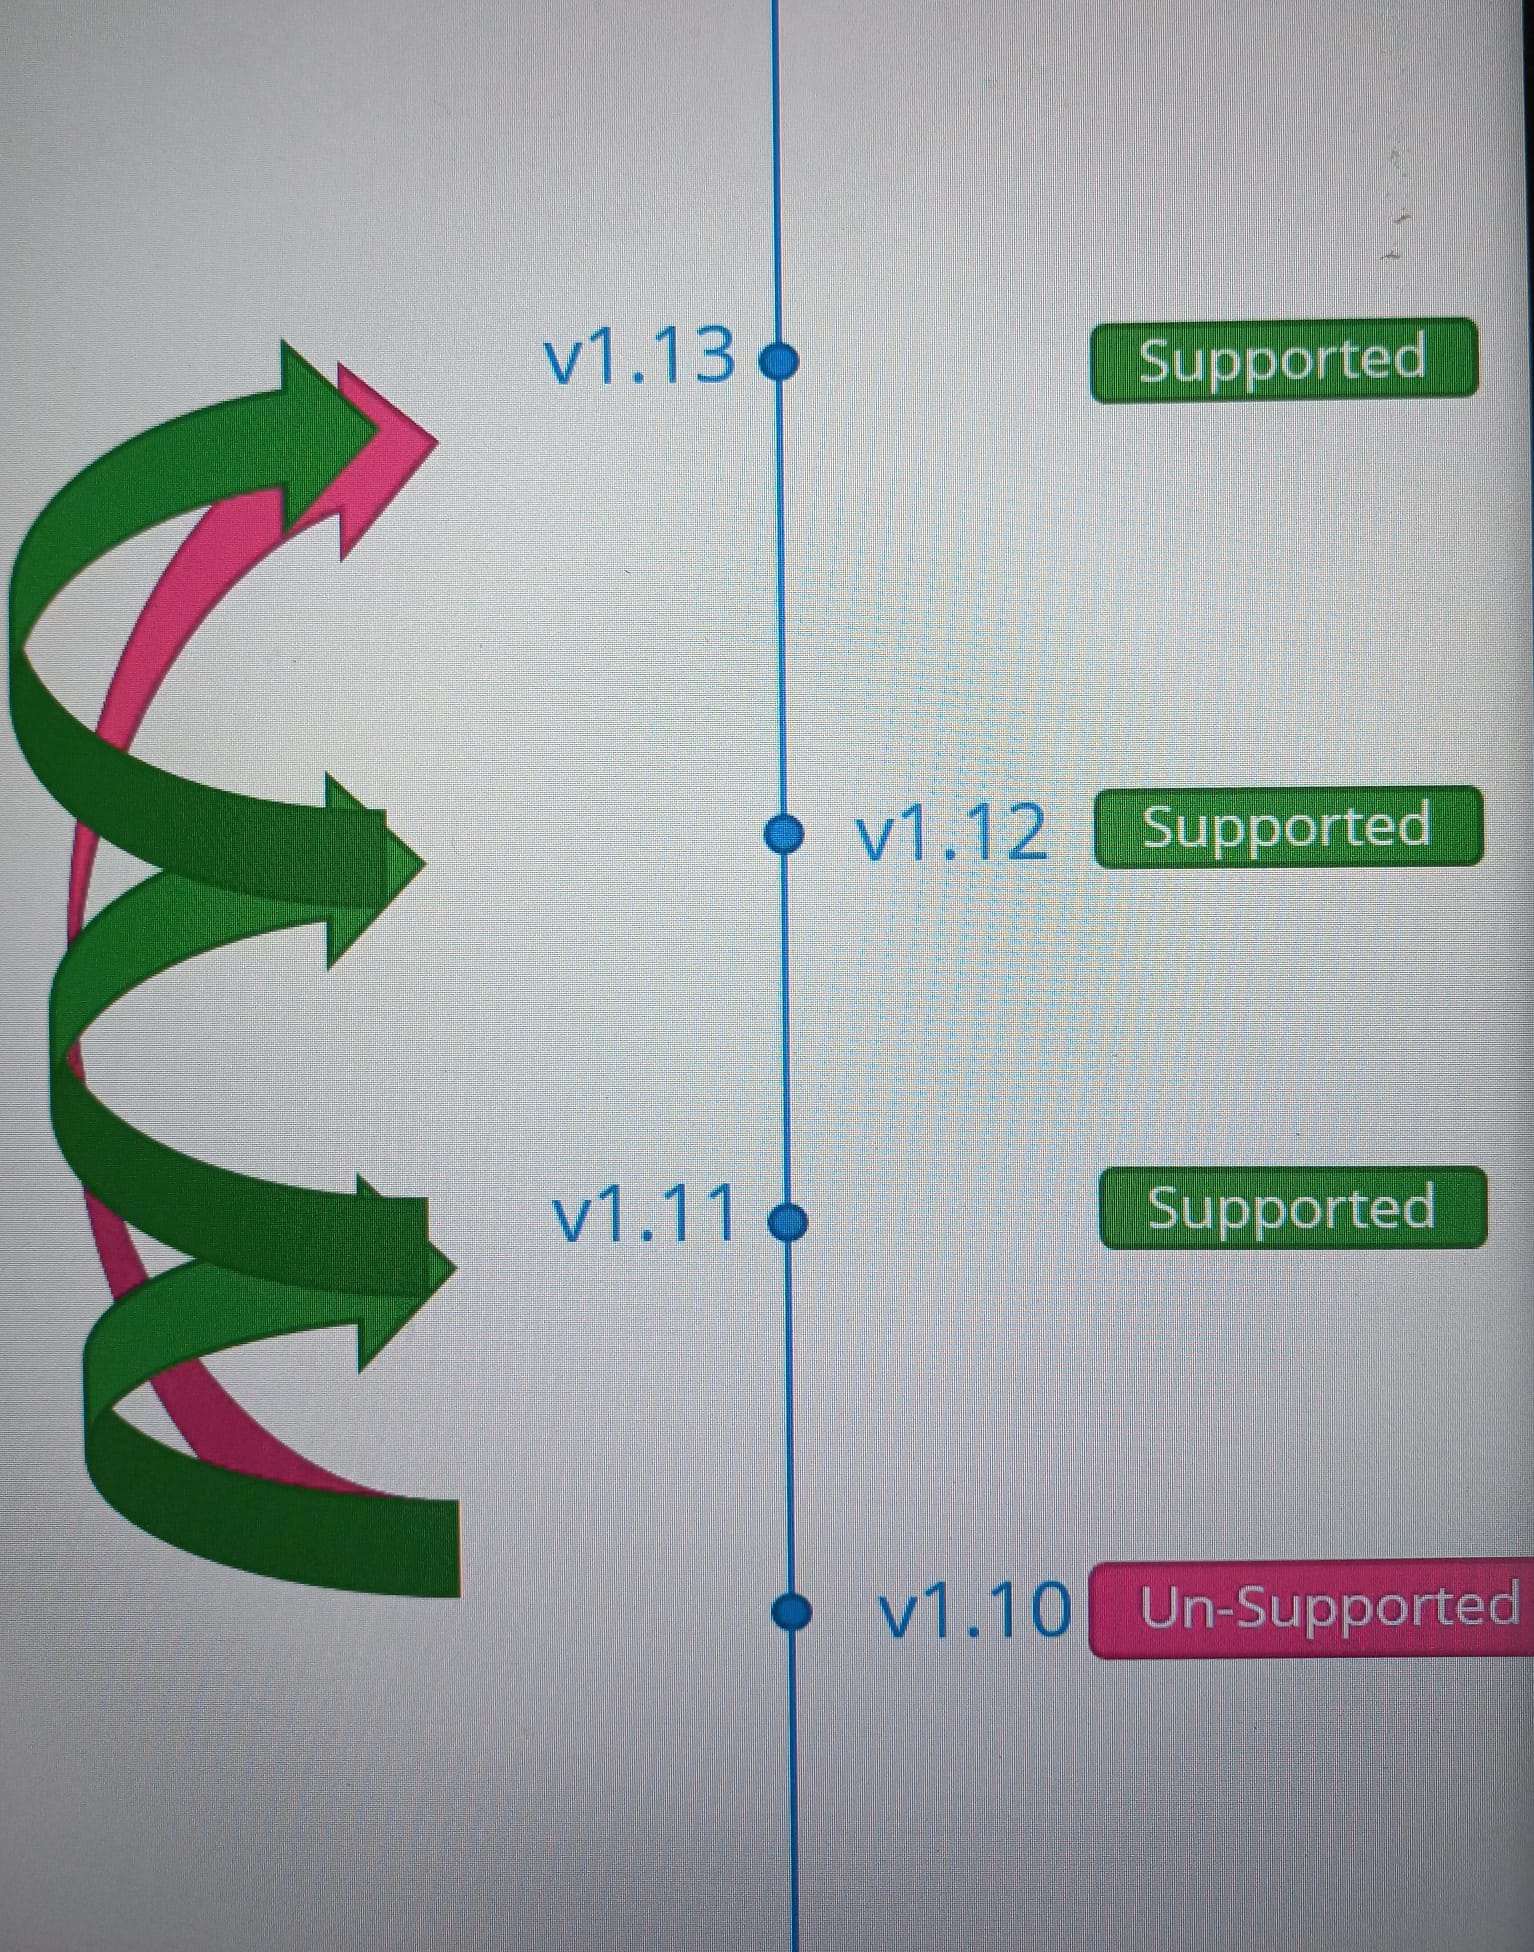
\includegraphics[scale=0.13]{pictures/clusup1.png}
\end{figure}

\paragraph{Kubeadmind Upgrade Plan}

Imagine we have a cluster with Master and Worker Nodes, with applications running in production, hosting Pods, serving users. At first they are upgraded the Master Nodes version and then the Worker Nodes versions. When Master Nodes goes down does not mean your Worker Nodes and applications on the Cluster are impacted. All workloads hosted on the Worker Nodes continue to serve users as normal, but all the management functions are down, so you cannot access the cluster using kubectl or other K8s API, so you cannot deploy new applications or modify existing ones.  But deployments and ReplicaSets are already running, so if a Pod fails, it is automatically deployed.

Once the Master Nodes are Upgraded, now it is time to upgrade Worker Nodes, there are different strategies to update Worker Nodes, one is update all of them at once, but this is not recommended, because all Pods are down and users are no longer able to access the applications. Once the update is completed, new Pods are scheduled and users can resume access.

The seconds strategy, the one recommended is to update one Node as a time, so when we update one node, the Pods that were running on it are automatically re-scheduled into another Nodes. So when a Node is upgraded, then the next one is updated and so on until the end.

\begin{codetemplate}{}
\begin{verbatim}
$ kubeadm upgrade plan
\end{verbatim}
\end{codetemplate}

With this command you can see the version of all components in the K8s Cluster. Also you can see the version which they can be updated. Finally it says that once you have upgrade the K8s components, you have to upgrade manually the kubelet on each Node.

\paragraph{Steps to upgrade K8s version from 1.11 to 1.13}

\begin{enumerate}

    \item Upgrade the kubeadmin version to version 1.12
\begin{codetemplate}{}
\begin{verbatim}
$ sudo apt-get upgrade -y kubeadm=1.12.0-00
\end{verbatim}
\end{codetemplate}

    \item Upgrade the Cluster
\begin{codetemplate}{}
\begin{verbatim}
$ kubeadm upgrade apply v1.12.0 -y
\end{verbatim}
\end{codetemplate}

    \item Get Nodes to see the Nodes version, it will still be in 1.11, because this command shows the version of the kubelets.
\begin{codetemplate}{}
\begin{verbatim}
$ kubectl get nodes
\end{verbatim}
\end{codetemplate}

    \item Go to the Master Nodes and upgrade kubelet version (if is has kubelet)
\begin{codetemplate}{}
\begin{verbatim}
$ sudo apt-get upgrade -y kubelet=1.12.0-00
\end{verbatim}
\end{codetemplate}
\begin{codetemplate}{}
\begin{verbatim}
$ systemctl restart kubelet
\end{verbatim}
\end{codetemplate}

    \item Move Pods workload of the first Worker Node to another Nodes
\begin{codetemplate}{}
\begin{verbatim}
$ kubectl drain node-1
\end{verbatim}
\end{codetemplate}

    \item Go to the Worker Node and upgrade the kubeadmin version
\begin{codetemplate}{}
\begin{verbatim}
$ sudo apt-get upgrade -y kubeadm=1.12.0-00
\end{verbatim}
\end{codetemplate}

    \item Now install and download the kubelet version:
\begin{codetemplate}{}
\begin{verbatim}
$ apt install kubelet=1.12.0-00 -y
\end{verbatim}
\end{codetemplate}
\begin{codetemplate}{}
\begin{verbatim}
$ sudo apt-get upgrade -y kubelet=1.12.0-00
\end{verbatim}
\end{codetemplate}
\begin{codetemplate}{}
\begin{verbatim}
$ kubeadm upgrade node config --kubelet-version v1.12.0
\end{verbatim}
\end{codetemplate}
\begin{codetemplate}{}
\begin{verbatim}
$ systemctl restart kubelet
\end{verbatim}
\end{codetemplate}
\begin{codetemplate}{}
\begin{verbatim}
$ kubectl uncordon node-1
\end{verbatim}
\end{codetemplate}

    \item Do the same for the rest of the Worker Nodes
\end{enumerate}

\begin{figure}[H]
    \includegraphics[width=\textwidth]{pictures/clusup2.png}
\end{figure}

\begin{blocktemplateIII}{WARNING}
If kubeadm or kubelet are not installed in the Node, at first it is needed to install them:
\begin{codetemplate}{}
\begin{verbatim}
$ sudo apt install kubelet=1.27.0-00
\end{verbatim}
\end{codetemplate}
\end{blocktemplateIII}

\begin{blocktemplateII}{NOTE}
If you are a cluster admin, and you need to access different nodes, you can use SSH to connect to them via their internal ip:
\begin{codetemplate}{}
\begin{verbatim}
$ kubectl get nodes -o wide
\end{verbatim}
\end{codetemplate}
\end{blocktemplateII}

\begin{blocktemplateI}{NOTE}
To know easily the IP of a Pod or the Node where it is running, you can use the following command:
\begin{codetemplate}{}
\begin{verbatim}
$ kubectl get po -o wide
\end{verbatim}
\end{codetemplate}
\end{blocktemplateI}

%==========================================================
\newpage
\section{Security}

%======================================================
\newpage
\section{Storage}

\subsection{Docker Storage}

\subsubsection{Introduction}

To understand the Storage in container orchestration tool like K8s, it is important to first understand how storage works with containers, for example in Docker containers. It makes so much easir to understand how it works in K8s.

When it comes to storage in Docker, there are two concepts you must know about:
\begin{itemize}
    \item Docker Storage Drivers and File Systems
    \item Volume Drivers
\end{itemize}

\subsubsection{Where does Docker stores its persistent data?}

in this lecture we are going to see where and how \textbf{Docker stores data} and how it manages \textbf{file systems} of the containers. Let's start with how Docker stores data on the local file system. When you install Docker on a system it creates this folders structure at \verb|/var/lib/docker/.|

\begin{codetemplate}{}
\begin{verbatim}
$ kubectl create -f service-template.yaml
\end{verbatim}
\end{codetemplate}\begin{codetemplate}{}
\begin{verbatim}
|- /var/lib/docker
       |- aufs/
       |- containers/
       |-  image/
       |-  ...
       | - volumes/
\end{verbatim}
\end{codetemplate}

This is where Docker stores all this data by default. Data as:

\begin{itemize}
    \item\textbf{image/:}  files with the data related to images stored on the Docker Host
    \item \textbf{containers/:} files with the data related to containers running on the Docker Host
    \item \textbf{volumes/:} files with the data related to any volumes created by the docker containers created
\end{itemize}

\subsubsection{Docker Image Layer Architecture}

But how does Docker exactly to store the files of an image and containers? We need to understand \textbf{Docker's layered architecture}. When Docker build images it does following a \textbf{layered architecture}, each line of instruction in the Dockerfile creates a new layer in the Docker image with just the changes from the previous layer.

\begin{figure}[H]
    \centering
    \includegraphics[scale=0.15]{pictures/st1.png}
\end{figure}

Since every layer \textbf{ONLY STORES THE CAHNGES FROM THE PREVIOUS LAYER, AND NOT ALL THEIR DATA} it is reflected in the size as well.

To understand the advantages of this layered architecture let's consider a second Dockerfile, which is different but in some parts is common. Using the same image, the same python and flask dependencies, but uses a different source code to create a different application image. When you run the \verb|docker build| command to build a new image for this application, since the first three layers of both the applications are the same, d\textbf{ocker is not going to build the first three layers}, instead it reuses the first 3 layers from the cache (generated with the build of the first Dockerfile). So only creates the last two layers. That is how Docker easily and efficiently saves disc space, and saves us a lot of time during builds and updates.

\begin{figure}[H]
    \centering
    \includegraphics[width=\textwidth]{pictures/st2.png}
\end{figure}

\begin{blocktemplateII}{NOTE}
Once the image is \textbf{completely build}, you cannot modify the contents of the layers, so they are \textbf{Read Only} and you can only modify them by iniciation a new build.
\end{blocktemplateII}

When you run a container based on this images with \verb|docker run| comman, it adds a new writeable layer on the TOP of the image layer, this layer is created to store data created by the container such as:

\begin{itemize}
    \item Logs files written by the applications
    \item Any temporary files generated by the container
    \item Just any file modified by the user on that container, or by external accessing
\end{itemize}

The life of this layer though is only as long as the container is alive. So when the container is destroyed, this layer and all of the changes stored on it are also destroyed. Remember that the same image layer is shared by all containers created using this image.

So imagine that we create a container, and in the runtime environment we want to create a file called temp.txt. It will be created in the container layer, but it won't take effect over Image Layers, so if you run a container with the same image, this file will not be created. Furthermore, if you for example modify the source code application that was created inside the Image Layer, it will only be modified in the Container Layer, so if you run another container with the same image the modification will not take effect. This is because when you modify some file in the Image Layer, Docker automatically creates a copy of that file in the Container Layer (it is invisible for the user but it happens), so you can play with this file as you want but never modify the image ones.

As we said, when a containers is destroyed, all the data stored in the Container Layer is automatically removed, the change in the app code, or the files we have created, all disappears. That's why we wanted to Persist the Data.

\subsubsection{Volumes in Docker}
\label{dockmount}
Imagine we want to create a DB container, so we obviously want to preserve the data created in the Container Layer, as long as it is a DB, and users, applications and other servers will be constantly modifying its content. So it has to be resilient to restarts, and independent to the containers created. If the container restarts it must have the data it has when he died, and all the containers running the DB image must have the same data, for data consistency. For that purpose, \textbf{Docker has Persisnt Volumes}.

\paragraph{Volume Mounting}

The first step is to \textbf{mount a Docker Volume}, to tell Docker to creates a folder:

\verb|/var/lib/docker/volumes/data_volume|:

\begin{codetemplate}{}
\begin{verbatim}
$ docker volume create data_volume
\end{verbatim}
\end{codetemplate}

Then have to pass it as an argument when you run the container:
\begin{codetemplate}{}
\begin{verbatim}
$ docker run -v data_volume:/var/lib/mysql mysql1.0.0
\end{verbatim}
\end{codetemplate}

So this way, we create a Symbolic Link between docker container path and our local path, so every change made by the database container will be written in the local folder. Even if the container is destroyed the data is still here.

\begin{blocktemplate}{NOTE}
But what would happen if you use the run command without having created a Docker volume previously?
\begin{codetemplate}{}
\begin{verbatim}
$ docker run -v data_volume_2:/var/lib/mysql mysql1.0.0
\end{verbatim}
\end{codetemplate}

Docker is so intelligent and will create before running the container the Persistent Volume, and then, create the link between the local folder and the container.
\end{blocktemplate}

To see all the Persistent Volumes created by Docker:
\begin{codetemplate}{}
\begin{verbatim}
$ docker volume ls
\end{verbatim}
\end{codetemplate}

Or:
\begin{codetemplate}{}
\begin{verbatim}
$ ls -la /var/lib/docker/volumes/
\end{verbatim}
\end{codetemplate}

To inspect specific volume:
\begin{codetemplate}{}
\begin{verbatim}
$ docker volume inspect volume_name
\end{verbatim}
\end{codetemplate}

\paragraph{Bind Mounting}

But what happen if we have our data already at another location? For example in our local folder, inside the application directory, under /data and we want to share this data as a volume with the container (maybe to do some tests), and not in the default \verb|/var/lib/docker/volumes/| folder. In this case we will use the docker run command with -v without creating a Volume, but in this case we must to provide the complete or relative path to the folder we would like to mount:

\begin{codetemplate}{}
\begin{verbatim}
$ docker run -v /users/titocampis/alexwork/appmysql/data:/var/lib/mysql mysql1.0.0
\end{verbatim}
\end{codetemplate}

\begin{codetemplate}{}
\begin{verbatim}
$ docker run -v data:/var/lib/mysql mysql1.0.0
\end{verbatim}
\end{codetemplate}

\paragraph{Volume Mounting vs Bind Mounting}

\textbf{Volume Mount:} It mounts a Volume from the volumes directory.

\textbf{Binding Mount:} It mounts a Volume from any other location in the Docker Host.

\paragraph{The correct way: run --mount}

\begin{blocktemplateI}{NOTE}
In the new versions of Docker, the correct way to mount a volume (Bind or not) inside a container is using the option \verb|--mount|
\begin{codetemplate}{}
\begin{verbatim}
$ docker run \
    --mount type=bind,source=/data/mysql,target=/var/lib/mysql \ 
    mysql:1.0.0
\end{verbatim}
\end{codetemplate}
\begin{codetemplate}{}
\begin{verbatim}
$ docker run \
    --mount type=mount,source=mydata,target=/var/lib/mysql \ 
    mysql:1.0.0
\end{verbatim}
\end{codetemplate}
\end{blocktemplateI}

\subsubsection{Storage Drivers \& Volume Drivers}

\paragraph{Storage Drivers}

But who is in charge to these operations? The \textbf{Storage Drivers}.

\begin{itemize}
    \item Maintining the layered architecture
    \item Creating a writable layer
    \item Moving files across layers to enable copy and write 
    \item etc.
\end{itemize}

Docker uses Storage Drivers to enable layered architecture, some of the common storage drivers are: AUFS, ZFS, BTRFS, Device Mapper, Overlay, Overlay2. The decistion of which use depens on the underlying SO (Ubuntu, IOS, Windows, etc.).

\paragraph{Volume Drivers}

\textcolor{red}{\textbf{PENDING}}

\subsection{K8s CSI (Container Storage Interface)}

In the past K8s used Docker alone as the container runtime engine, and all the code to work with Docker was embedded within the K8s Cluster source code. But with other container runtimes comming ins as: Rocket and CRI-O, it was important to open up and extend support to work with different container runtimes and no be dependent on the K8s source code. And that's why \textbf{Container Runtime Interface (CRI)} came to be. It is a standard that defines how an orchestration solution like K8s would communicate with container runtimes like Docker, so in the future if a new container runtime interface is developed, they can simplify follow the CRI standards and that new container runtime would work with K8s.

It is similary to the extension of CNI (Container Networking Interface), to extend the support for different Networking Solutions. Now any Networking vendors could simply develop their plugin based on the CNI standards and make their solution work with K8s.

\begin{figure}[H]
    \includegraphics[width=\textwidth]{pictures/st3.png}
\end{figure}

So as you can imagine, CSI (Container Storage Interface) was developer to support multiple storage solutions, with CSI you can now write your own drivers for your own storage to work with K8s. Port Works, Amazon EBS, Azure Desk, etc. Everyone's got their own CSI drivers.

\textcolor{red}{\textbf{PENDING}, you also have to describe a little bit this rules to build you solution and suits K8s}

\subsection{K8s Volumes \& Persistent Volumes}

\subsubsection{Docker Volumes}

Docker containers are meant to be transient in nature, which means they are meant to last only for a short period of time. They are designed to process, recieve, modify and do thing with this data but destroy all data once finished, the data is destroyed along with the container. To persist data processed by the containers we attach a volume to the container when they are created, as we saw in section \ref{dockmount}. 

So the data processed by containers are now stored in this volume, retaining it permanently.

\begin{figure}[H]
    \includegraphics[width=\textwidth]{pictures/st4.png}
\end{figure}

\subsubsection{K8s Volumes}

How does it works in K8s world? Just as in Docker, the Pods created on K8s are transient in nature, when a pod is created it manages data and when it is destroyed, all its data is destroyed as well. \textbf{In order to persist data, we attach Volumes to the Pods}, so data generated by the POd is now stored in the Volume, and even after the Pod is deleted, the data remains.

\paragraph{Creating a K8s Volume}

Imagine we have a Pod that runs an image inside a container which has a command that generates a random number and stores it under \verb|/opt/number.out|. If the Pod is generated without a volume, the data will be stored inside the Pod, but when the Pod dies, the data will be removed.

\textbf{.spec.volumes}

In order to retain the number generated by the Pod, we create a \textbf{volume} inside the Pod in  \textbf{.spec.volumes}. There are multiple configurations, but for now, we are going to configure it to use a directory on the host. This way all the files stored in the directory on the Pod will be stored in the directory data on the Node where the Pod is running.

\textbf{.spec.containers.volumeMounts}

But that's not all,  we have to mount this volume inside the container in order to container can use it.

\begin{codetemplate}{}
\begin{verbatim}
apiVersion: v1
kind: Pod
metadata:
    name: random-number-generator
spec:
    containers:
    - image: alpine
      name: alpine
      command: ["/bin/bash","-c]
      args: ["shuf -i 0-100 -n 1 >> /opt/number.out;]
      ...
      volumeMounts:
      - mountPath: /opt
        name: data-volume
    volumes:
    - name: data-volume
      hostPath:
        path: /data
        type: Directory
\end{verbatim}
\end{codetemplate}

Now yes, the random number will be written in the \verb|/opt/number.out| container directory and in the Node directory \verb|/data|. When the Pod dies, the random number file still lives on the Node.

But you can imagine this is not suitable, because if the Pod restarts and now is allocated in another Node, the data will be lost!! Because it is only on the last Node. For that the solution involves 2 actors:

\begin{itemize}
    \item \textbf{Use external shared storage solutions to share storage between nodes:} K8s supports several types of different shared storage solutions as:
    \begin{itemize}
        \item NFS
        \item GlusterFS
        \item Flocker
        \item Ceph
        \item AWS
        \item Azure
        \item Google Persisent
    \end{itemize}

    \item \textbf{Use Persistent Volumes for }
\end{itemize}

\paragraph{Example of use external shared storage solution}

If we are using the AWS shared storage solution:
\begin{codetemplate}{}
\begin{verbatim}
...
volumes:
- name: data-volume
  awsElasticBlockStore:
    volumeID: <volume-id>
    fsType: ext4
\end{verbatim}
\end{codetemplate}

\subsubsection{K8s Persistent Volumes}

\href{https://kubernetes.io/docs/concepts/storage/persistent-volumes/}{Official K8s Doc}

It is a way of manage the storage more centrally, you would like it to be configured in a way that an administrator can create a large pool of storage and then have users carve out pieces from it as required. That is where \textbf{Persistent Volumes} can help.

A Persistent Volume is a cluster-wide pool of storage volumes configured by an administrator to be used by users deploying applications on the cluster. The users can now select storage from this pool using \textbf{Persistent Volume Claims}

\begin{figure}[H]
    \includegraphics[width=\textwidth]{pictures/pv.png}
\end{figure}

\paragraph{Creating a Persistent Volume}

\begin{codetemplate}{pv-template.yaml}
\begin{verbatim}
apiVersion: v1
kind: PersistentVolume
metadata:
    name: pv-vol1
spec:
    accessModes:
    - ReadWriteOnce
    capacity:
        storage: 1Gi
    hostPath:
        path: /tmp/data
\end{verbatim}
\end{codetemplate}

\textbf{accessMode}

Defines how a volume should be mounted on the hosts, read-only, read-write, etc. The supported values are:
\begin{itemize}
    \item \textbf{ReadOnlyOnce:} the PV will be read-write by a single node, it only can be read from resources inside the same node.
    \item \textbf{ReadOnlyMany:} the PV will be read-only by resources in many nodes.
    \item \textbf{ReadWriteMany:} the PV will be the volume read-write by many nodes.
\end{itemize}

\begin{blocktemplateIII}{WARNING}
hostPath option must not be used in Production Environments, because it means you are associating the storage of the current Node where you are creating the Persistent Volume.

To avoid that, you can replace with one of the supported storage solutions as we saw in the previous lecture, for example:
\begin{codetemplate}{pv-template.yaml}
\begin{verbatim}
...
    capacity:
        storage: 1Gi
    awsElasticBlockStore:
        volumeID: <volume-id>
        fsType: ext4
\end{verbatim}
\end{codetemplate}

\end{blocktemplateIII}

\begin{codetemplate}{}
\begin{verbatim}
$ kubectl create -f pv-template.yaml
\end{verbatim}
\end{codetemplate}

\begin{codetemplate}{}
\begin{verbatim}
$ kubectl get pv
\end{verbatim}
\end{codetemplate}

\subsection{K8s Persistent Volume Claims}

\href{https://kubernetes.io/docs/concepts/storage/persistent-volumes/#persistentvolumeclaims}{Official K8s Doc}

As we saw in the previous lecture, \textbf{Persistent Volume Claims} are the K8s objects that makes \textbf{Persistent Volumes} available on the Nodes. PV's and PVC's are two separate objects in the K8s Namespace. An administrator creates a set of PV'se, and a user creates PVC's to use the storage.

\begin{blocktemplateIII}{WARNING}
PV's are not attached to any Namespace, they are across all Namespaces, but it can have permisions of view depending on the role. It is recommended to only have read-writte acces to this objects by Cluster Aminsitrators.
\end{blocktemplateIII}

Once the PVC's are created, K8s binds (vincula) the PV's to claims based on the request and properties set on the volume. Every PVC must be bounded to a single PV, during the binding process, K8s tries to find a PV that matches the following requests of the PVC's:

\begin{itemize}
    \item has sufficient capacity
    \item has same access modes
    \item has same volume modes
    \item has same Storage Class
\end{itemize}

However, if there multiple possible matches for a single claim, and you would like to specifically use a particular PV, you could still use \textbf{labels and selectors} to bind to the right PV's.

\begin{blocktemplateIII}{WARNING}
Remember the relationship between PV's and PVC's is one to one, so there cannot be more than one PVC binded to a PV. If the PVC requires less storage than the PV storage, no toher PVC's can uses the remaining capacity in the volume. If there are not available Volumes that matches the PVC, it will remain in a Pending State until newe volumes are made available on the Cluster, and when that happens, the PVC is automatically bounded.
\end{blocktemplateIII}

\subsection{Creating a Persistent Volume Claim}

\begin{codetemplate}{pvc-template.yaml}
\begin{verbatim}
apiVersion: v1
kind: PersistentVolumeClaim
metadata:
    name: myclaim
spec:
    accessModes:
    - ReadWriteOnce
    resources:
        requests:
            storage: 500Mi
\end{verbatim}
\end{codetemplate}

\begin{codetemplate}{}
\begin{verbatim}
$ kubectl get pvc
\end{verbatim}
\end{codetemplate}

\begin{blocktemplate}{NOTE}
If we pay attention on what we see when get pvc, we can see the PV attached to that pvc.
\end{blocktemplate}

\paragraph{Deleting Persistent Volume Claims}

Just use the  \verb|kubectl delet pvc <name>| command. But what happens with the underlying PV? You can choose what is to happen to the PV. By defaul it is set to retain, meaning the PV will remain until it is manually deleted by the administrator and it is not available for reuse by any other claims anymore, it is so romantic.

Also, you can change the default configuration:

\begin{codetemplate}{pv-template.yaml}
\begin{verbatim}
apiVersion: v1
kind: PersistentVolume
metadata:
    name: pv-vol1
spec:
    accessModes:
    - ReadWriteOnce
    capacity:
        storage: 1Gi
    hostPath:
        path: /tmp/data
    persistentVolumeReclaimPolicy: Recycle
    # Default persistentVolumeReclaimPolicy: Retain
    # persistentVolumeReclaimPolicy: Delete
\end{verbatim}
\end{codetemplate}

If you use \textbf{Delete} option the PV will be deleted as soon as the PVC is deleted, freeing up storage on the end storage device. If you use \textbf{Recycle} the data in the data volume will be scrubbed before making it available to other claims.

\paragraph{Associating PVC's to Pods to containers can cosume them}

Once you create a PVC use it in a POD definition file by specifying the PVC Claim name under persistentVolumeClaim section in the volumes section like this:

\begin{codetemplate}{}
\begin{verbatim}
apiVersion: v1
kind: Pod
metadata:
    name: random-number-generator
spec:
    containers:
    - image: alpine
      name: alpine
      command: ["/bin/bash","-c]
      args: ["shuf -i 0-100 -n 1 >> /opt/number.out;]
      ...
      volumeMounts:
      - mountPath: /opt
        name: data-volume
    volumes:
    - name: data-volume
      persistentVolumeClaim:
        claimName: myclaim
\end{verbatim}
\end{codetemplate}

\subsection{Application Configuration}

\subsection{Lab - Playing with PV's \& PVC's}

\textbf{To see the content of a file it is lighter to do:}

\begin{codetemplate}{}
\begin{verbatim}
$ kubectl exec -it <pod-name> -- cat /path/to/the/file
\end{verbatim}
\end{codetemplate}

\begin{blocktemplateIII}{WARNING}
It is not necessary to create a PV object to share storage bare between a Pod and the Node. It's enough to create volume in the specs of the Pod an a volumeMount in the container, and you will do the same it does docker, in your system. 

But this only applies to bare shared storage between a Node an a Pod, if you want to persist the storage between all Nodes it is more complex, so you have to create PV's and PVC's.
\end{blocktemplateIII}

A hardly recommendation is that when the change is little, you can do it with \verb|kubectl edit| command, but when it is hard, use:

\begin{codetemplate}{}
\begin{verbatim}
$ kubectl get po webapp -o yaml > pod.yaml
\end{verbatim}
\end{codetemplate}

Then edit the template and delete and create the new Pod with the changes, it has more verbose and tolerance to errors.

Once did it, you can look at the Node directory associated and see if it is used or not by the Pod, and actually yes, it doeees!!!!!!!

\begin{codetemplate}{}
\begin{verbatim}
$ cat /var/log/webapp
\end{verbatim}
\end{codetemplate}

\subsubsection{Question 9}

\begin{codetemplate}{}
\begin{verbatim}
$ kubectl get pvc -o yaml | grep -i access -A 5
\end{verbatim}
\end{codetemplate}

\begin{codetemplate}{}
\begin{verbatim}
$ kubectl get pv -o yaml | grep -i access -A 5
\end{verbatim}
\end{codetemplate}

OR:

\begin{codetemplate}{}
\begin{verbatim}
$ kc get pvc -o jsonpath='{..accessModes}'
\end{verbatim}
\end{codetemplate}

\begin{blocktemplateIII}{WARNING}
If there is storage let over in the PV, the PVC will get in all.
\end{blocktemplateIII}

\begin{codetemplate}{}
\begin{verbatim}
$ kubectl get pvc
===> CAPACITY: 100Mi
\end{verbatim}
\end{codetemplate}

\subsubsection{Question 12}

Only need to modify volumes in the pod-template.yaml.

\begin{blocktemplateIII}{WARNING}
The PVC must be in the same Namespace as the Pod, if it is not like that, it won't work.
\end{blocktemplateIII}

\begin{blocktemplateII}{IMPORTANT}
With this solution, the logs of the application will be available on every Node on the cluster!
\end{blocktemplateII}

\subsubsection{Question 16}

\begin{blocktemplateIII}{WARNING}
If you try to delete a PVC used by a Pod, it won't be definitely deleted until the Pod dies. In will remain in Terminating state.
\end{blocktemplateIII}


\subsubsection{Question EXTRA}

\textbf{What happens if we modify, remove, or add files to the shared directory?}

Wow, if you add files in the local directory they are added automatically to the pod:

\begin{figure}[H]
    \includegraphics[width=\textwidth]{pictures/wow.png}
\end{figure}

Y lo mismo sucede al reves!!! WOOOOOW!!! Quedan automagicamente conectados para siempre. Amigos para siempre do you want to be my friend...

\begin{figure}[H]
    \includegraphics[width=\textwidth]{pictures/amigosparasiemrep.png}
\end{figure}
\begin{figure}[H]
    \includegraphics[width=\textwidth]{pictures/amigosforever.png}
\end{figure}



\subsection{Storage Class}

In the previous lectures, we discussed about how to create PV's an then create PVC's to claim that storage, and then use the PVC's in the Pod definition files as volumes. The problem here is before the PV's are created disk storage must be created on the Cloud Platform (Google, Azure, IBM, AWS, etc.). So every time an application requires storage it is needed to manually provision the disk and after create manually a PV using the definition file using the same name as the disk you have already created. This is called static provisioning volumes.

It will be amazing if the volume is provisioned automatically when the application requires it, and that is where \textbf{StorageClass} come in. With \textbf{StorageClass} you can define a provisioner like google storage which automatically provision storage on the cloud and attach that to Pods when the claim is made. It is called dynamic provisioning on Pods. You do that by creating an Object \textbf{StorageClass}.

\begin{codetemplate}{sc-template.yaml}
\begin{verbatim}
apiVersion: storage.k8s.io/v1
kind: StorageClass
metadata:
    name: object-storage
provisioner: kubernetes.io/gce.pd
\end{verbatim}
\end{codetemplate}

We use the provisioner \verb|kubernetes.io/gce.pd| to create a Volume on GCP. There are other any provisioners as well, as AWS EBS, Azure File, Azure Disk, Portworx, etc. With each of these provisioners, you can pass in additional parameters such as the type of disk to provision, the replication type, etc. These parameters are very specific to the provisioner that you are using.

If we use \textbf{StorageClass} we no longer need the PV definition, because the PV and any associated storage is going to be associated automatically when the StorageClasses created. But we have to let the PVC know about the StorageClass, so:

\begin{codetemplate}{}
\begin{verbatim}
apiVersion: v1
kind: PersistentVolumeClaim
metadata:
    name: claim-log-1
spec:
    accessModes:
    - ReadWriteOnce
    storageClassName: <name-of-storage-class>
    resources:
        requests:
            storage: 50Mi
\end{verbatim}
\end{codetemplate}

With this definition, the \textbf{StorageClass} associated to the PVC uses the defined provisioner to provision a new disk with the required size.

\begin{blocktemplateIII}{WARNING}
The \verb|storageClassName| works similarly to accessMode, if the PVC has one defined, it cannot be bound to a PV that has another one defined or which does not have any defined. PV and PVC accessMode must match. 
\\\\
If the PVC has no accessMode it cannot be assignet to a PV defined with an accessMode.
\end{blocktemplateIII}

\begin{blocktemplateIII}{WARNING}
If the Storage Class makes use of VolumeBindingMode set to WaitForFirstConsumer, it will delay the binding and provisioning of a PersistentVolume until a Pod using the PersistentVolumeClaim is created.
\end{blocktemplateIII}

\subsubsection{Different Storage Classes}
One thing that is common is to use different \textbf{StorageClasses} deppending on the package that the enterprise or applications purchase. For example:

\begin{figure}[H]
    \includegraphics[width=\textwidth]{pictures/stcl.png}
\end{figure}

%======================================================
\newpage
\section{Networking Basis in Linux (not K8s)}

\subsection{Switching and routing in Linux}
\label{swrt}

\subsubsection{Switching}

What is a network? We have 2 Linux Machines, A and B, it can be: laptops, desktops, VMs on the Cloud, wherever. How does system A reach system B? So we connect them to a \textbf{switch} and it creates a network containing the two systems. 

\begin{figure}[H]
    \includegraphics[width=\textwidth]{pictures/ntw.jpg}
\end{figure}

To connect the 2 Linux machines to a switch, we need an interface on each host (physical or virtual depending on the Host). And to see the interfaces from the Host, we use the following command:

\begin{codetemplate}{}
\begin{verbatim}
$ ip link
\end{verbatim}
\end{codetemplate}

We only want the information of \textbf{eth0} interface, which it will be used to connect the machine to the switch. 

Let's assume it's a Network with the adress 192.168.1.0, so we then assign the system with IP addresses on the same Network:

\begin{figure}[H]
    \includegraphics[width=\textwidth]{pictures/ntw2.png}
\end{figure}

\begin{codetemplate}{}
\begin{verbatim}
$ ip addr add add 192.168.1.10/24 dev eth0
\end{verbatim}
\end{codetemplate}

Once the links are up and the IP addresses are assigned, the computers can now communicate with each other through the switch. The switch can only enable communication within a Network, which means it can receive packets from a Host on the Network and deliver it to other systems within the same Network.

Imagine we have another2 machines in another Network at adress 192.168.2.0 and system adress according to this adress. How does a system in one Network reach a system in another Network?

\begin{figure}[H]
    \includegraphics[width=\textwidth]{pictures/ntw3.png}
\end{figure}

Once the links are up and the IP addresses are assigned, the computers can now communicate with each other through the switch. The switch can only enable communication within a Network, which means it can receive packets from a Host on the Network and deliver it to other systems within the same Network.

\subsubsection{Routing}

Imagine we have another2 machines in another Network at adress 192.168.2.0 and system adress according to this adress. How does a system in one Network reach a system in another Network?

Using \textbf{Routers}, a \textbf{Router} is an intelligent device which can connect two networks together. Is like another server with a lot of \textbf{Network Ports}. Since it connects to the two separate Networks it gets 2 IPs assigned, one on each Network, for example:

\begin{itemize}
    \item For the first Network, it receives the IP: 192.168.1.1
    \item For the second Network, it receives the IP: 192.168.2.1
\end{itemize}

\begin{figure}[H]
    \includegraphics[width=\textwidth]{pictures/ntw4.png}
\end{figure}

Imagine that system A wants to communicate with system C. How does the system A know where the Router is configured on the Network to send the packages through? The router is just another device set on the Network with an associated IP. This is why we configure the systems with a \textbf{gateway} or a \textbf{route}. If the Network was a room, the \textbf{gateway} would be the door to the external world (other Networks). The systems need to know where that door is. 

\textbf{See existing routing configuration on a system:} it displays the kenel's routing table
\begin{codetemplate}{}
\begin{verbatim}
$ route
\end{verbatim}
\end{codetemplate}

If nothing is configured, system A cannot go outside its Network, so it cannot communicate with system C or D, only with D.

\textbf{To configure a gateway in system A:}
\begin{codetemplate}{}
\begin{verbatim}
$ ip route add 192.168.2.0/24 via 192.168.1.1
\end{verbatim}
\end{codetemplate}

Specifing that to reach 192.168.2.0/24 Network, it should pass through 192.168.1.1 (the router).

As you can imagine, we have to do the same for system B, to reach system C and system D. And the same for systems C and D to reach systems A and B. Configuring a route on the Network and configure routes on the systems.

Now supose these systems need access to the internet, for example to google at 172.217.194.0. You only need to connect the router to the internet and add a new route to the systems, to pass through router to go to Google (172.217.194.0). But there are so many different sites on different Networks on the internet, so instead of adding a routing table entry for the same router's IP adress, for each of those Networks, \textbf{we can simply say for any Network that you do not know where to route, use this router as the default gateway}. And that's the key.

\begin{codetemplate}{}
\begin{verbatim}
$ ip route add default via 192.168.2.1
\end{verbatim}
\end{codetemplate}

\begin{blocktemplate}{NOTE}
Instead of the word "default" we can use 0.0.0.0, which means any IP destination.
\end{blocktemplate}

This way, any request to an IP outside of your existing Network (not defined in route table) goes to this particular router. 

\subsubsection{Private and Public Networks configuration}

So in a simple model like this, all you need is a single routing table entry with the default gateway set to the router's IP address. But if we want to manage connections with another private Network at the same time than Public Network (as internet), it gets complicated. We should have 2 routers with 2 route rules in the configured system tables, to use different routers to send the traffic depending on the Network systems want to reach.

\begin{figure}[H]
    \includegraphics[width=\textwidth]{pictures/ntw5.png}
\end{figure}

\begin{itemize}
    \item One rule to connect to internal private Network on router 1
\begin{codetemplate}{}
\begin{verbatim}
$ ip route add 192.168.1.0/24 via 192.168.2.2
\end{verbatim}
\end{codetemplate}

    \item Another rule to connect to all other Networks (including internet)
\begin{codetemplate}{}
\begin{verbatim}
$ ip route add default via 192.168.2.1
\end{verbatim}
\end{codetemplate}
\end{itemize}

\subsubsection{Using a Linux System as a router}

\begin{figure}[H]
    \includegraphics[width=\textwidth]{pictures/ntw6.png}
\end{figure}

As you know, Host A has no idea of how to reach Host C, because it is into another Network. So we have to say Node A to reach Host C through Node B. So we do that adding a routing rule in the table of Host A:

\begin{codetemplate}{}
\begin{verbatim}
$ ip route add 192.168.2.0/24 via 192.168.1.6
\end{verbatim}
\end{codetemplate}

When the Host C wants to response Host A will have the same issue, so we have to do the same on Host C:
\begin{codetemplate}{}
\begin{verbatim}
$ ip route add 192.168.1.0/24 via 192.168.2.6
\end{verbatim}
\end{codetemplate}

If we try to ping now, we no longer get the Network unreachable error message, that means our routing entries are right, but we still do not get any response back. This is because by deafult, in linux, packets are not forwarded from one interface to the next. For example: packets received on Eth0 of Node B are not forwarded to elsewhere thorught Eth1, for obviously security reasons. But in this case, that we know they are both secure Networks, and we want to use Node B as router, we can allow Host B to forward packets  from one Network to the other. It is set in a file on the system config:

\begin{codetemplate}{}
\begin{verbatim}
$ cat /proc/sys/net/ipv4/ip_forward
\end{verbatim}
\end{codetemplate}

\begin{itemize}
    \item \textbf{0:} No forward
    \item \textbf{1:} Forward
\end{itemize}


\begin{codetemplate}{}
\begin{verbatim}
$ echo 1 > /proc/sys/net/ipv4/ip_forward
\end{verbatim}
\end{codetemplate}

\begin{blocktemplateIII}{WARNING}
This way of configuration is not resilient to reboot, so if the system is reboot the configuration will be lost. To persist the configuration you should configure that in /ect/sysctl.conf adding:
\begin{codetemplate}{}
\begin{verbatim}
$ sudo vim /ect/sysctl.conf
###############################
...
net.ipv4.ip_forward=1
...
\end{verbatim}
\end{codetemplate}

\end{blocktemplateIII}

\subsection{DNS in Linux}

\subsubsection{Introduction to DNS}

We have 2 Hosts in the same Network, Host A and Host B. And they have been assigned a Network with IP: 192.168.1.0. So they are 192.168.1.10 and 192.168.1.11. So as we saw in the last section \ref{swrt}. As they are in the same Network, they can reach each other using their IP's. But it can be so tediously for Hosts to know all the IP's, so instead of having to remember the IP address of system B, Host A can give it a name, for example db, that when you \verb|ping db| it works like if it was using IP.

Basically we want to tell Host A that system B at IP address at 192.165.1.11 has a name db. So when db name is used, for Host A must be the same as 192.165.1.11. It can be done by adding an entry in the file \verb|/etc/hosts|:

\begin{codetemplate}{}
\begin{verbatim}
$ echo "192.168.1.11      db" >> /etc/hosts
\end{verbatim}
\end{codetemplate}

Or vim and add at the end of the file the relationship.
\begin{codetemplate}{}
\begin{verbatim}
$ sudo vim /etc/hosts
\end{verbatim}
\end{codetemplate}

So now Host A translates db as 192.165.1.11, this is called \textbf{name resolution}, associate a hostname to an IP. Whatever we put in the \verb|/etc/hosts| is the source of true for the Host. But that my not be the truth, maybe Host B is called host-2, but Host A does not care, it will follow what is in the \verb|/etc/hosts| file. 

You can make a test, associate \verb|www.google.com| hostname to IP of Host B an tst to ping, the ping will be answered by Host B. You can have any names as you want for any servers as you want in the \verb|/etc/hosts| file. Commands look into this file:

\begin{itemize}
    \item ping
    \item ssh
    \item curl
    \item nc
    \item nmap
    \item mtr
    \item ...
\end{itemize}

\subsubsection{DNS server}

In a system with few systems, you can get away with the entries of \verb|/etc/hosts| file, and this is how it was done in the past. However, when the environment grows and these files got filled with many entries you can imagine this is unmanageable. If one of the Hosts changes its IP, you are done, gj wp. This is the reason why it was decided to \textbf{move all this configuration into a single server}, who will manage all this centrally, called the \textbf{DNS server}. And then we point all hosts to look up that server if they need to resolve a hostname to an IP address instead of its own \verb|/etc/hosts| files.

How do we do that? How de we point our host to a DNS server? Imagine our DNS server has the IP 192.168.1.100, every host has a DNS resolution configuration file at \verb|/etc/resolv.conf|. So you have to add an entry into it specifying the address of the DNS server.

\begin{codetemplate}{}
\begin{verbatim}
$ echo "nameserver         192.168.1.100" >> /etc/resolv.conf
\end{verbatim}
\end{codetemplate}

Or vim and add it at the end of the file.
\begin{codetemplate}{}
\begin{verbatim}
$ sudo vim /etc/resol.conf
\end{verbatim}
\end{codetemplate}

Once this is configured into a Host, everytime it comes up across a hostname that it does not know about, it looks it up from the DNS server. With this configuration, if the IP of any of the host was to change, you only need to change it in one file in one Host.

\begin{blocktemplateIII}{WARNING}
You can still have entries in your \verb|/etc/hosts| file, but it is not hardly recommended because it will override the configuration in \verb|/etc/resolv.conf| nameserver. Only use it when you are sure of what you are doing.
////
But this is default configuration, this order can be changed in the file \verb|/etc/nsswitch.conf|
\begin{codetemplate}{}
\begin{verbatim}
$ cat /etc/nsswitch.conf
\end{verbatim}
\end{codetemplate}

\textbf{OUTPUT:} hosts:    files dns

To change this, you should modify the content on the field to invert it.
\end{blocktemplateIII}

What happens if the hostname is not found in \verb|/etc/hosts| neither in \verb|/etc/resolv.conf|, so it will fail. Unless you configure in the file \verb|/etc/hosts| of the \textbf{DNS server} to forward all unknown hostnames to the public name server on the internet (ex: 8.8.8.8).

\begin{codetemplate}{}
\begin{verbatim}
$ echo "Forward All to 8.8.8.8" >> /etc/hosts
\end{verbatim}
\end{codetemplate}

\subsubsection{FQDN}

So far, we are naming with names like db, host-1, host-2... But the real services are called: www.google.com, www.github.com, etc. They are using \textbf{FQDN's}.

\textbf{FQDN} (Fully Qualified Domain Name) or \textbf{Domain Name}, which are a complete and unique direction needed to have presence on the internet. It is composed by the name of the host and the domain, and it is used to request to specific hosts on the internet using the name resolution instead of their IP.

Let's see a FQDN structure in detail:

\begin{figure}[H]
    \centering
    \includegraphics[scale=0.4]{pictures/image11.PNG}
\end{figure}

\begin{enumerate}
    \item \textbf{TLD (Top Level Domains):} they represent the intent or the geographical situation of the website:
    \begin{itemize}
        \item \textbf{.com:} for commercial or general purpose
        \item \textbf{.net:} for network
        \item \textbf{.edu:} for educational organizations
        \item \textbf{.es / .cat / .fr:} for geographical situation
        \item \textbf{.org:} for non-profit organizations
    \end{itemize}

    \item \textbf{Domain:} it is the hostname assigned to Google
    \item \textbf{Name of the host:} is a subdomain, which helps in further grouping things together under the Domain, for example:
    \begin{itemize}
        \item \textbf{maps.google.com:} the maps of google
        \item \textbf{drive.google.com:} the drive of google
        \item \textbf{www.google.com:} google search
        \item \textbf{mail.google.com:} google email
    \end{itemize}
\end{enumerate}

But how does this magical works in all Hosts in the world, for exampe the PC we are using. This is because when your system tries to reach any of these \textbf{FQDN's} your system first check at your \textbf{internal DNS server (on routeer)}, and it normally does not know who apps or google is, so it forwards your request to the internet. On the internet the IP adress of the server for example \textbf{maps.google.com} may be resolved with the help of \textbf{multiple DNS servers}. A \textbf{root DNS server} looks at your request and points you to a DNS server, which serves at (.com) TLD. So this \textbf{.com DNS servers} looks at your request and forwards it to \textbf{Google}, and \textbf{Google's DNS server} provides your system the IP of the server serving the maps.

But as this is so tedious, your \textbf{local DNS server (router)} may choose to cache this IP for a period of time, typically few seconds up to few minutes. That way, it does not have to go throught the whole process again each time.


\subsubsection{Creating own FQDN}

Imagine we want to expose a service to the internet with different sub-services, like a pay service, a consult service, a book service, a message service, etc. And do you want to access them on the internet by FQDN names and not IP's, so common. You must have an \textbf{internal DNS server}, and you must configure the hostname-IP relationship in its \verb|/etc/hosts| file.

So when you want to access your service from inside the Network from any host, the host at first will look in its local configuration file \verb|/etc/hosts|, then if nothing finds it will look in the \textbf{DNS server} configured in the \verb|/etc/resolv.conf|, whichi will tell you that pay.myapp.com is the IP 192.68....

But we can one step further, inside my private network, maybe I want to use the servicde without the FQDN, because it is very long, maybe I want to use it by web, it is easier. Is this possible? The answer is yes, you must make an entry into your host's \verb|/etc/resolv.conf|:

\begin{codetemplate}{}
\begin{verbatim}
search mycompany.com
\end{verbatim}
\end{codetemplate}

Next time you try to ping web, you will see it actually tries web.mycompany.com. As if you try pay, it will try pay.company.com.

\subsubsection{Record Types (Tipos de Registros)}

How are the records stored in the DNS server?

\begin{itemize}
    \item \textbf{hostname to IP:} A records
    \item \textbf{hostnames to IPv6:} AAAA records
    \item \textbf{Mapping one name to another name:} CNAME records. For example, you may have multiple aliases for the same application (maps.google.com = car.google.com, walk.google.com, cycle.google.com, etc.) and that's why a CNAME record is used, name to name mapping.
\end{itemize}

\subsubsection{Nslookup or dig}
One of the best tools for \textbf{DNS name resolution} is \textbf{nslookup}. Instead of ping, you can use the binary nslookup to query a hostname from a DNS server, but remember that nslookup does not consider the entries in the local \verb|/etc/hosts| file. Nslookup only queries the DNS server. The same happens with the binary \textbf{dig}, another useful tool to tes DNS name resolution

\subsection{Network Namespaces in Linux}

\subsubsection{Introduction to Namespaces in Linux}

Network Namespaces in Linux are used by containers like Docker to implement Network isolation, as we know \textbf{containers are separated from their underlying host using Namespaces}, but what are Namespaces? You can imagine Host is a house, and the Namespaces are the different rooms you assing to each of your child, to have certain privacy and independence, so the kids can only see their own room, they cannot see what happens in other room or in the rest of the house (they are isolated). However, as a parent, you ahve visibility into all the rooms in the house as well as other areas of the house. if you wish, you can stablish connectivity between two rooms in the house.

When you create a container you want to make sure that it is isolated, that it does not see any other processes on the host or any other containers, so we create a special room for it on our host using a Namespace, so the container only sees the processes run by it and thinks that it is on its own host XD. Nevertheless, the underlying host has visibility into all of the processes including those running inside containers. This can be seen listing system processes.

\begin{itemize}
    \item If you list the system processes on a running container, you will see only the processes executed by the container and the container process itself
\begin{codetemplate}{}
\begin{verbatim}
$ ps waux
\end{verbatim}
\end{codetemplate}

    \item If you list the system processes on the underlying host you will see all the other processes runing in the host (a lot)
\begin{codetemplate}{}
\begin{verbatim}
$ ps waux
\end{verbatim}
\end{codetemplate}
\end{itemize}

\subsubsection{Namespaces for Networking}

When we create a container, our host has its own routing and ARP tables with information about res of the Network. We want to seal all of those deatils from the container, so when the container is created, we create a Network Namespace for it, that way it has no visibility to any network-related information on the host. Within its Namespace, the container can have its own virtual interfaces, routing and ARP tables, the container has its own interface.

This section is very complicated, it is explained to understand how docker manage the Network of its container, I won't document this part, because it can be an entire lecture by itself. Anyhow, if you want to know more information, check the associated video in the CKA Course.

%======================================================
\newpage
\section{Networking in K8s}

\subsection{Docker Networking}

Same as in the last section, this section is very complex and it only helps to understand how docker manage the network, for more information check the video assoaciated.

\subsection{CNI (Container Networking Interface)}

As we have seen in the previous lecture, isolate container Network is so hard, and this task is carried out by every software of containerization like: docker, rkt, mesos, K8s. All of them \textbf{associate containers to a Bridge Network (Namespace)} using the Bridges and IP / Routing isolation concepts we saw in the previous lecture.

So, someone smart, thought to externalize the functionality, and create a binary called \textbf{bridge} which creates an isolated Namespaces automatically with only one command. This binary is used by K8s, docker, mesos, etc. When a container starts, the binary is executed to create a Bridge Network (Namespace) where the container will run.

But this program is not closed, it has some configurations for the user to configure its own custom networks. That's where CNI (Container Network Interfaces) comes in. CNI is a set of standards that define how programs have to be defined to solve networking challenges in a container runtime environments. The programs are referred to as plugins, Bridge program is a plugin for CNI.

CNI defines a set of responsabilities  for container runtimes and pluggins. All the container manage systems can use these CNI's to define their networks, except Docker.\textbf{Docker does not implement CNI}, Docker has its own set of standards known as CNM which stands for container network model which is another standard similar to CNI but with some differences.

So when K8s run a docker container it runs it with \textbf{non-Network} and then invokes the configured CNI plugins who take care of the rest of the configuration

\subsection{Networking Cluster Nodes}

The K8s Cluster consists of Master and Worker Nodes, each node must have at least one interface connected to a Network and each interface must have an address configured. The hosts must have a unique host name set, as well as a unique MAC adress.

\begin{figure}[H]
    \centering
    \includegraphics[scale=0.2]{pictures/locura1.png}
\end{figure}

Also, the Nodes must have the following ports opened:

\underline{Worker Nodes}
\begin{itemize}
    \item \textbf{10250:} kubelet
    \item \textbf{30.000 - 32.767:} services
\end{itemize}

\underline{Master Node}
\begin{itemize}
    \item \textbf{6443:} Kube-apiserver
    \item \textbf{10250:} kubelet
    \item \textbf{10251:} Kube-scheduler
    \item \textbf{10252:} Kube-controller-manager
    \item \textbf{2379:} etcd-cluster
\end{itemize}

\begin{figure}[H]
    \includegraphics[width=\textwidth]{pictures/ports.png}
\end{figure}

\begin{blocktemplate}{NOTE}
Yes, a kubelet can be present on the Master Node. An if you have multiple Master Nodes all these ports need to be open those as well, and also need a \textbf{port 2380} to connect both \textbf{etcd-clients}
\end{blocktemplate}

\subsubsection{Useful Commands}

\begin{codetemplate}{}
\begin{verbatim}
$ ip link
\end{verbatim}
\end{codetemplate}

\begin{codetemplate}{}
\begin{verbatim}
$ ip addr
\end{verbatim}
\end{codetemplate}

\begin{codetemplate}{}
\begin{verbatim}
$ ip addr add 192.168.1.10/24 dev eth0
\end{verbatim}
\end{codetemplate}

\begin{codetemplate}{}
\begin{verbatim}
$ ip route
\end{verbatim}
\end{codetemplate}

\begin{codetemplate}{}
\begin{verbatim}
$ ip route add 192.168.1.0/24 via 192.168.2.1
\end{verbatim}
\end{codetemplate}

\begin{codetemplate}{}
\begin{verbatim}
$ ip route add deault via 192.168.2.1
\end{verbatim}
\end{codetemplate}

\begin{codetemplate}{}
\begin{verbatim}
$ cat /proc/sys/net/ipv4/ip_forward
\end{verbatim}
\end{codetemplate}

\begin{codetemplate}{}
\begin{verbatim}
$ arp
\end{verbatim}
\end{codetemplate}

\begin{codetemplate}{}
\begin{verbatim}
$ netstat -plnt
\end{verbatim}
\end{codetemplate}

\subsubsection{Lab - Playing with Networking in K8s Cluster}

\textcolor{red}{\textbf{PENDING}}

\subsection{POD Networking Concepts}

As we have seen, Master and Worker Nodes are configured to share the same Network, so they can reach each other. We also made sure the firewall and network security groups are configured correctly to allow for the K8s control plane components to reach each other. Supposing we have also set up all the K8s control plane components such as the kube-apiserver, etcd servers, kubelets, etc. Before applications can run, there is something that we must adress. We have talked about the Network that connects the Nodes,  but there is also another layer of networking that is crucial to the clusters functioning, and that is the networking at the Pod layer. Our K8s cluster is soon going to have a large number of Pods and services running on it, how are the Pods adressed? How do they communicate eachother? Internally inside the cluster and externally outside the cluster?

These are challenges that K8s expects you to solve, as of today, K8s do not come with a built-in solution for this. It expects you to implement a Networking Solution that solves this challenges. Nevertheless, K8s have laid out clearly the requirements for Pod Networking:

\begin{itemize}
    \item Every Pod have an IP Adress
    ...
\end{itemize}

More information in the video section.

\textcolor{red}{\textbf{PENDING}} It is so complicated, continue when you have time.

A nivel general me quedo con el concepto de que en cada nodo se monta una red privada, rollo bridge a la cual se conectan todos los pods que en el nodo corren. Cada pod toma una IP de esa red privada y metiante esa red se comunican todos los pods que se ejecuten en un nodo. Para que los pods puedan comunicarse con pods de otros nodos, se establece un router a nivel de la red privada del cluster, que es otra red diferente a la red de los nodos, pero que se indica a cada nodo que reenvien las peticiones hacia esa red si no encuentran el host, y a partir de ahi, esta encamina hacia el resto de Nodos.

\subsection{CNI in K8s}

CNI defines the responsabilities of container runtime.. Continua el rollazo

\textcolor{red}{\textbf{PENDING}}

\subsection{WeaveWorks Solution (based on CNI)}

\textcolor{red}{\textbf{PENDING}}

\subsection{IPAM (CNI)}

\textcolor{red}{\textbf{PENDING}}

\subsection{Service Networking}

\subsubsection{Introduction}

IN previous lectures we have talked about Pods Networking, how bridge networks are created within each node and how pods get a namspace created for them, and how interfaces are attached to those namespaces, and how Pods get an IP adress assigned to them within the subnet assigned for that Node.

We also saw through routes, we can get the Pods on different Nodes to talk to each other forming a large Virtual Network where all Pods can reach each other. But it is so rare to configure Pods to communicate directly with each other (todo este rollazo para nada, diosmio). \textbf{Normally, when you want a Pod to access apps hosted on another Pod you would always use a Service object.}

So, if a Pod wants to consume an app, it only have to use the IP assigned to its Service or the Service name. It does not matter if it a Pod from the same Node, because when a Service is created it is accessible from all Pods on the Cluster. Because a Service is hosted across the cluster, not bound to a specific Node. 

\begin{blocktemplateIII}{WARNING}
All the Services are accessible by each resource inside the cluster by its name or its IP, but it is not accessible from outside the Cluster, because its IP belongs only to the Virtual Internal Network of K8s    
\end{blocktemplateIII}

The more basic Service configuration is of type \textbf{ClusterIP}. \textbf{NodePort} does exactly the same as \textbf{ClusterIP} Service but in addition, it exposes the application on a port on all Nodes in the Cluster. This way, external users can use the service connecting directly with nodes IP's.

\subsubsection{How services works, kube-proxy}

So our focus must be more on Services than in Pods, how are these Services getting these IP addresses? And how are they made available across all the Nodes in the Cluster? How is the service made available to external users throuhg a port on each Node? The responsible is \textbf{kube-proxy} element, which is running into every Node on the Cluster.

\textbf{Kube-proxy} element watches the changes in the cluster through kube-apiserver and every time a new service is to be created, kube-proxy gets into action. Unlike Pods, Services are not created on each Node or assigned to a Node, \textbf{Services are Cluster-wide concept}. They exists across all the Nodes in the Cluster. As a matter of fact, they do not exist at all. Besides, there are no processes, bridges, namespaces or interfaces for a Service, it is just a virtual object. 

So how do they get an IP adress? And how are we able to access the application on a Pod through a Service? \textbf{When we create a service object in K8s it is assigned an IP address from a predefined range}. The \textbf{kube-proxy} components running on each node gets that IP address and creates forwarding rules on each Node saying: "Any traffic comming to this IP should go to the IP of the Pod". Once that is in place, whenever a pod tries to rach the IP of the Service it is forwarded to the Pod's IP address, which is accessible from any Node in the Cluster (as we have discussed in previous lectures). But remember, it is not just an IP, it is an IP and a Port combination, whenever Services are created or deleted \textbf{kube-proxy} component of each Node creates or delete these rules.

\subsubsection{How kube-proxy set that rules?}

kube-proxy supports different ways to set networking rules:

\begin{itemize}
    \item \textbf{userspace:} kube-proxy listens on a port
    \item \textbf{ipvs rules}
    \item \textbf{iptables (default):} as we saw in section \ref{swrt}
\end{itemize}

The kube-proxy can be set using the proxy mode option, default is iptables:

\begin{codetemplate}{}
\begin{verbatim}
$ kube-proxy --proxy-mode [userspace | iptables | ipvs] ...
\end{verbatim}
\end{codetemplate}

\subsubsection{Example of iptable rule application}

\textcolor{red}{\textbf{PENDING NTAP redirection}}

\subsection{DNS on K8s}

So imagine we have 3 Nodes in our K8s cluster with Pods and services running. Each node has a nodenam and IP adressassignet to it. The Node names and IP adresses  of the Cluster are probably registered in a DNS server in your organization, and how accesse them are not of concern in this lecture, in this lecture we will discuss the DNS resolution within the cluster, between different components such as Pods and Services.

K8s deploys a \textbf{built-in DNS server} by default when you setup a cluster, if you run k8s from scratch, you have to do it by yourself. We focus purely on pods and services within the cluster, we are not interested on Nodes FQDN. 

Let's se this example:

\begin{figure}[H]
    \centering
    \includegraphics[width=\textwidth]{pictures/ingress1.png}
\end{figure}

Looking at the Pods IP's you should notice that it would be running on different Nodes, but this is not important, because all Pods and Services can reach each other using their IP addresses. So to make the webserver Pod accessible to other Pods we use a Service.

Whenever a Service is created, the \textbf{K8s DNS Server} creates a record for the Service, mapping the Service name with its IP address. So within the Cluster, any Pod can reach now the newly created Service using its service name. \textbf{Remember that the Service name can change if the Pod who is calling it is in the same Namespace or in another Namespace}

\begin{itemize}
    \item \textbf{Pod in the same Namespace:} service-name
    \item \textbf{Pod outside the Service Namespaces:} service-name.namespace
\end{itemize}

For each Namespace the \textbf{K8s DNS Server} creates a Sub domain, all the Services are group together into another Sub Domain called \textbf{svc}, so you can reach your application using \textbf{service-name.namespace-name.svc}. Additionally, all resources in a Cluster are group together into a route domain for the cluster \textbf{cluster.local}, so you can also reach your application using the URL which is the FQDN \textbf{service-name.namespace-name.svc.cluster.local}. So as you see, \textbf{Services} are the suitablle objects to consume apps within the Cluster.

Records for Pods are not created by default, but we can enable it explicitly. But once a Pod is created, \textbf{K8s DNS Server} creates a record for the Pod, exactly equal to the IP of the Pod but with dashes (10.3.4.0 : 10-3-4-0), \textbf{Namespace} is the same and type is pod. Soto access directly a pod you can use: \textbf{pod-ip-dashes.namespace-name.pod.cluster.local}

\subsubsection{How K8s Implements DNS in the Cluster}

In this lecture we will see how K8s makes possible to reach a Service or a Pod from another Pod. So if you have 2 or 3 Pods, you only have to configure the \verb|/etc/hosts| file to add the mapping. But as in a Cluster can be thousands of hundreds of Pods it is not feasible. Instead we move these entries into a \textbf{Central K8s DNS Server}. We have to add this \textbf{DNS Server} to the Pods configuration file \verb|/etc/resolv.conf| specifing that the nameserver is at the IP address of the \textbf{Central K8s DNS Server}. Every time a new Pod or Service is created we add a record in the DNS server for that Pod so the other Pods can access the new Pod or Service with their FQDN, and the new Pod can also resolve other Pods in the Cluster.

\begin{figure}[H]
    \centering
    \includegraphics[width=\textwidth]{pictures/ingress2.png}
\end{figure}

K8s implement DNS in the same way, it deploys a \textbf{DNS Server} within the Cluster, it must be CoreDNS. But how is CoreDNS setup in the Cluster. It is deployed as a Pod in the \textbf{kube-system Namespace}, actually it is created as two Pods for redundancy as par of a ReplicaSet and a Deployment. This Pod runs \textbf{CoreDNs executable} the same executable we should run if we create our cluster from scratch. It requires a configuration file named Corefiled located on \verb|/etc/coredns/Corefile|

\begin{figure}[H]
    \centering
    \includegraphics[scale=0.2]{pictures/ingress3.png}
\end{figure}

This file is charged into a \textbf{ConfigMap in the K8s kube-admin Namespace}

\subsubsection{How Pods point to the CoreDNS Server?}

What adress do the Pods use to reach the \textbf{DNS Server}?

\textcolor{red}{\textbf{PENDING NTAP redirection}}

\subsection{Ingress}

\href{https://kubernetes.io/docs/concepts/services-networking/ingress/}{Official K8s Doc}

\subsubsection{The need of Ingress}

 Imagine you are deploying an application on K8s for a company that has an online store selling products, your application would be available at my-online-store.com. You build your application into a docker image, and run it in your K8s Cluster in a Pod, into a Deployment. Your application also needs a DB, so you deploy a MYSQL DB as a Pod and create a service of type ClusterIP, called mysql-service to make it accessible by our application.

 So the application is now working, and it connects with the mysql-service properly, but how can we make the application accessible to the outside world? At first you have to create another service, to homogenize the application under a stable IP insided the cluster, with load balancing. It does not matter, but imagine that you create your Service NodePort type with nodePort=38080, so you make your application available on an IP within the cluster and on a static Pod in every Node of the Cluster.

 \begin{figure}[H]
    \centering
    \includegraphics[width=\textwidth]{pictures/ingress4.png}
\end{figure}

 So actually, \textbf{users can access to the application using the url} \verb|http://IP_OF_ONE_RANDOM_NODE:38080|. This incredibly works, and users are able to acces the application. But as you can imagine it is not very suitable.

 Imagine that the traffic increases, so it increase the number of replicas to handle the additional traffic. That's not a problem because the Service take care of splitting traffic between the Pods. However if you have deployed a production-grade application before, there are many more things involves in addition to simply splitting the traffic between the pods. 
 
 For example, we do not want users to have to type in the IP adress every time, so you to solve this, you can configure your DNS Server to point to the IP of the Nodes, so the user can now access the application using the URL \verb+http://my-online-store.com:38080+.

 We do not want to that the user have to remember port number either, however service nodePorts can  only allocate high numbered ports. So you have to add some piece between the user and the service who maps the port 80 to port 38080 on your Nodes. You then point your DNS to this server and users can now access the application by simply visiting \verb|my-online-store.com|

Imagine that you deploy your application in for example Google Cloud. You could instead of creating a Service of type NodePort you can create it as type LoadBalancer. When you do that, K8s will do the same that i has to do for a NodePort, which is creating a virtual ip for the Service accessible within all the Cluster and provision a high port for the service in all Cluster Nodes. But in addition to that, K8s also sends a request to Google Cloud Platform to provision a network load balancer for the Service. On receiving th request, Google Cloud Platform will then automatically deploy a load balancer configured to route traffic to the Service ports on all nodes.

The load balancer has an external IP that can be provided to users to access the application. In this case we can set the \textbf{DNS Server} to point to this IP and users access the application using the URL my-online-store.com

\begin{figure}[H]
    \centering
    \includegraphics[width=\textwidth]{pictures/ingress6.png}
\end{figure}

Your company grows and you now have new services for your customers, for example, a video streaming service. Now you want your users to be able to access your new video streaming service by going to my-\textbf{online-store.com/watch} and you want your old application be accessible now at \textbf{online-store.com/wear}. But they are actually two different microservices or directly applications. So you deploy your new application as a separate Pod, Deployment and Service (called video-service of type LoadBalancer) and K8s provision support 38282 for this Service and also provision a Network LoadBalancer on the Cloud. The new LoadBalancer has a new IP and remember that you must pay for each of these load balancers and having many such loadBalancers can inversely affect your Cloud Bill. 

So how do you direct traffic of these LoadBalancers based on the URL that the users type in. You need yet another proxy or LoadBalancer that can redirect traffic based on URL to the different Services. And every time you introduce a new Service you have to reconfigure the LoadBalancer. In addtion, you should enable SSL for your applications so your users can access your application using https. Where do you configure that? It can bedone at different levels: 

\begin{itemize}
    \item Application Level
    \item Load Balancer Level
    \item Proxy Server Level
\end{itemize}

But you want to configure that in one place with minimal maintenance.

\begin{figure}[H]
    \centering
    \includegraphics[width=\textwidth]{pictures/ingress7.png}
\end{figure}

So when the Cluster scales it becomes unmanageable, it would be nice if K8s manage all of that within the K8s Cluster and have all that configuration in just another configuration file that lives along with the rest  of your application Deployment and Services files. And this exists and they are Ingress.

\subsubsection{Introduction to Ingress}

\textbf{Ingress} helps users to access your application using a single externally accessible URL that you can configure to route traffic to different services within your Cluster based on the URL path. At the same time, implement SSL security as well. Think of \textbf{Ingress} as a layer 7 LoadBalancer built in the K8s Cluster that can be configured using native K8s primitives just like any other Object.

Even with \textbf{Ingress} you still \textbf{need to expose it to make it accessible outside the Cluster}, so you still have to either \textbf{publish it as a NodePort or with a Cloud-native LoadBalancer}. But that is just a one-time configuration. Going forward, you are going to perform all your load balancing of SSL and URL-based routing configuration on the \textbf{Ingress-Controller}.

\subsubsection{Ingress Controller \& Ingress Resources}

But what is an Ingress? Where it is? How can you see it, and how can you configure it? Without Ingress all its works would be done with a proxy-reverse or a LoadBalancer like NGINX, HAproxy, etc. It will be deployed in the K8s Cluster and configure them to route traffic to another services, with user routes, SSL certificates, endpoint services, etc.

\textbf{Ingress} are implemented by K8s in a very similar way, the \textbf{product deployed} by K8s is called \textbf{Ingress Controller} (is a product like NGINX), and the \textbf{set of rules} you configure are called \textbf{Ingress Resources}. \textbf{Ingress Resources} are created using definition YAML files. 

\subsubsection{Ingress Controller}

K8s Clusters does not come with an Ingress Controller by default, so you only create Ingress Resources and you expect it works, it won't. Soy you must deploy one.

There are a number of solutions available for \textbf{Ingress Controller:}
\begin{itemize}
    \item \textbf{GCE:} Google Controller layer 7 HTTP Load Balancer
    \item \textbf{NGINX}
    \item \textbf{Istio}
    \item \textbf{HAPROXY}
    \item \textbf{Treafic}
\end{itemize}

Currently, \textbf{GCE} and \textbf{NGINX} are currently being supported and maintained by the K8s project, and in this lecture we will use NGINX as an example. This Ingress Controller are not just another Load Balance or NGINX server, the Load Balancer components are just part of it. Ingress Controllers have additional \textbf{intelligence} to \textbf{monitor} the K8s Cluster for \textbf{new} definitions of \textbf{Ingress Resources} and configure the \textbf{NGINX Server accordingly}. A \textbf{NGINX Controller} is deployed just as another deployment in K8s.

To run \textbf{properly} an \textbf{Ingress Controller} in your K8s Clsuter you should \textbf{create} the following resources:

\begin{itemize}
    \item \textbf{Deployment} with an Ingress Controller Image to run into containers
    \item \textbf{ConfigMap} to configure the NGINX
    \item \textbf{Service} type NodePort to expose it
    \item \textbf{ServiceAccount} with the right permission to access all of these objects
\end{itemize}

\paragraph{Deployment}

\begin{codetemplate}{nginx-ingress-controller.yaml}
\begin{verbatim}
apiVersion: extensions/v1beta1
kind: Deployment
metadata:
    name: nignx-ingress-controller
spec:
    replicas: 1
    selector:
        matchLabels:
            name: nginx-ingress
    template:
        metadata:
            labels:
                name: nginx-ingress
        spec:
            containers:
            - image: quay.io/kubernetes-ingress-controller/nginx-ingress-controller:0.21.0
              name: nginx-ingress-controller
            args:
            - /nginx-ingress-controller
            - --configmaps=$(POD_NAMESPACE)/nginx-configuration
            env:
            - name: POD_NAME
              valueFrom:
                fieldRef:
                    fieldPath: metadata.name
            - name: POD_NAMESPACE
              valueFrom:
                fielRef:
                    fieldPath: metadata.namespace
            ports:
            - containerPort: 80
              name: http
            - containerPort: 443
              name: https
            
\end{verbatim}
\end{codetemplate}

Within the image, the NGINX program is stored at location \verb|/nginx-ingress-controller| so you must pass that as the command to start the NGINX controller service. Also, NGINX has more configurations like:
\begin{itemize}
    \item Path to store the logs
    \item Keep alive threshold
    \item SSL settings
    \item Session timeout
\end{itemize}

Also NGINX server need the env configuration to run properly and to specify the ports used by the Ingress Controller, which happens to be 80 for http connections and 443 for secure (https) connections.

\paragraph{ConfigMap}

In order to decouple this configuration data from the NGINX Controller Image we must create a ConfigMap Object:

\begin{codetemplate}{nginx-configuration.yaml}
\begin{verbatim}
apiVersion: v1
kind: ConfigMap
metadata:
    name: nginx-configuration
\end{verbatim}
\end{codetemplate}

You can let it blank if you want, it would apply the configuration by default, but it would make easy for you to modify a configuration setting in the future.

\paragraph{Service}

We then need a Service to expose the Ingress Controller to the external world, so we create a Service of type NodePort with the nginx-ingress label selector to link the service to the Deployment:

\begin{codetemplate}{}
\begin{verbatim}
apiVersion: v1
kind: Service
metadata:
    name: nginx-ingress
spec:
    type: NodePort
    ports:
    - port: 80
      targetPort: 80
      protocol: TCP
      name: http
    - port: 443
      targetPort: 443
      protocol: TCP
      name: https
    selector:
        name: nginx-ingress
\end{verbatim}
\end{codetemplate}

\paragraph{ServiceAccount}

As we said before, the Ingress Controllers have additional intelligente built into them to monitor the K8s Cluster for Ingress Resources and configure the underlying Ingress Controller when something is changed. But for the Ingress Controller to do this, it requires a Service Account with the right set of permissions: Roles, ClusterRoles and RoleBindings

\begin{codetemplate}{}
\begin{verbatim}
apiVersion: v1
kind: ServiceAccount
metadata:
    name: nginx-ingress-serviceaccount
\end{verbatim}
\end{codetemplate}

\subsubsection{Ingress Resources}

\href{https://kubernetes.io/docs/concepts/services-networking/ingress/}{Official K8s Doc}

An Ingress Resource is a set of rules and configurations applied on the \textbf{Ingress Controller}, you can configure rules to say simply forward all incoming traffic to a single application or route traffic to different applications based on URL, so if the user  goes to my-online-store.com/wear then route to one app, or if the user visits the my-online-store.com/watch then route to another app. Or you can route user based on the domain name itself, for example wear.my-online-store.com and watch.my-online-store.com

The Ingress Resource Objects are created with a YAML definition file, this one for example routes all the incoming traffic in the Cluster to the \textbf{wear-service Service} on \textbf{port 80}:

\begin{codetemplate}{ingress-wear.yaml}
\begin{verbatim}
apiVersion: extensions/v1beta1
kind: Ingress
metadata:
    name: ingress-wear
spec:
    backend:
        serviceName: wear-service
        servicePort: 80
\end{verbatim}
\end{codetemplate}

Then create it:

\begin{codetemplate}{}
\begin{verbatim}
$ kubectl create -f ingress-wear.yaml
\end{verbatim}
\end{codetemplate}

\begin{codetemplate}{}
\begin{verbatim}
$ kubectl get ingress
\end{verbatim}
\end{codetemplate}

\paragraph{Rules}

You can use rules when you want to route traffic based on different conditions. For example, you can create one route for traffic originating from each domain or hostname. 

That means when users reach your cluster using:

\begin{itemize}
    \item domain name my-online-store.com, you can handle that traffic using rule 1.
    \item domain name wear.my-online-store.com you can handle that traffic using rule 2.
    \item domain name watch.my-online-store.com you can handle that traffic using rule 3.
    \item use rule 4 to handle everything else.
\end{itemize}

And as we discussed before, you could\textbf{ get different domain names} to reach the Cluster by \textbf{adding multiple DNS entries} all \textbf{pointing} to the same \textbf{Ingress Controller Service} on the K8s Cluster.

So within each rule, you can define different paths and backend Services which serves in this hostnames.

So let's define rules:

\begin{codetemplate}{ingress-wear.yaml}
\begin{verbatim}
apiVersion: extensions/v1beta1
kind: Ingress
metadata:
    name: ingress-wear
spec:
    rules:
    - http:
        paths:
        - path: /wear
          backend:
            serviceName: wear-service
            servicePort: 80
        - path: /watch
          backend:
            serviceName: watch-service
            servicePort: 80 
    backend:
        serviceName: wear-service
        servicePort: 80
\end{verbatim}
\end{codetemplate}

\begin{blocktemplate}{NOTE}
If you use the command describe in one Ingress object you will see that there is a field called \textbf{Default backend}, what's that? If a user tries to access a URL that does not match any of these rules, then the user is redirected to the service specified as the \textbf{default backend}
\end{blocktemplate}

But this configures all the URL's that the user uses, what if you want to use different rules for each URL?

\begin{codetemplate}{ingress.yaml}
\begin{verbatim}
apiVersion: networking.k8s.io/v1
kind: Ingress
metadata:
    name: ingress-wear
spec:
    rules:
    - host: wear.my-online-store.com
      http:
        paths:
        - backend:
            serviceName: wear-service
            servicePort: 80
    - host: watch.my-online-store.com
      http: 
        paths:
        - backend:
            serviceName: watch-service
            servicePort: 80
    backend:
        serviceName: wear-service
        servicePort: 80
\end{verbatim}
\end{codetemplate}

So in this case the path is indiferent, what really matters is the URL that the users uses to access to the application. It depende on how application whats to manage their services. However, you can specify in addition different paths to this configuration to add more complexity to the configuration.

\paragraph{Ingress Resources updates in last K8s Versions}

\begin{enumerate}
    \item \textbf{apiVersion:} as changed to networking.k8s.io/v1
    \item \textbf{pathType:} there are 3 path types
    \begin{itemize}
        \item \textbf{Exact:} Matches the URL path exactly and with case sensitivity
        \item \textbf{Prefix:} Matches based on a URL path prefix split by /. Matching is case sensitive and done on a path element by element basis. A path element refers to the list of labels in the path split by the / separator.
        \item \textbf{ImplementationSpecific:} With this path type, matching is up to the IngressClass. Implementations can treat this as a separate pathType or treat it identically to Prefix or Exact path types.
    \end{itemize}
    \item \textbf{serviceName \& servicePort}
\end{enumerate}

\textbf{How does pathType Works?}
\begin{table}[H]
\begin{tabular}{| m{2.5cm} | m{2cm} | m{3.5cm} | m{4cm} |}
\hline
\textbf{Kind} & \textbf{Path(s)} & \textbf{Request Path} & \textbf{Matches?} \\ \hline
Prefix & / & (all paths) & Yes \\ \hline
Exact & / & (all paths) & No, only matches "/" \\ \hline
Prefix & /bar & /bar, /bar/temp & Yes \\ \hline
Exact & /bar & /bar, /bar/temp & No, only matches "/bar" \\ \hline
Exact & /bar/ & /bar, /bar & No, only matches "/bar/" \\ \hline
Prefix & /bar/ & /bar & Yes \\ \hline
Prefix & /wear & /watch & No, uses default backend \\ \hline
Prefix & /, /wear & /watch & Yes, it match "/" \\ \hline
Exact & /, /wear & /watch & No \\ \hline
Exact & /, /wear & / & Yes \\ \hline
\end{tabular}
\end{table}

\begin{codetemplate}{ingress.yaml}
\begin{verbatim}
apiVersion: extensions/v1beta1
kind: Ingress
metadata:
    name: ingress-wear
spec:
    rules:
    - host: wear.my-online-store.com
      http:
        paths:
        - pathType: Prefix
          path: /
          backend:
            service:
                name: wear-service
                port:
                    number: 80
    - host: my-online-store.com
      http: 
        paths:
        - pathType: Prefix
          path: /watch
          backend:
            service:
                name: watch-service
                port:
                    number: 80
        - pathType: Prefix
          path: /
          backend:
            service:
                name: watch-service
                port:
                    number: 80
\end{verbatim}
\end{codetemplate}

\paragraph{kubectl create ingress in the last versions}

\begin{codetemplate}{}
\begin{verbatim}
$ kubectl create ingress --help
\end{verbatim}
\end{codetemplate}

\begin{codetemplate}{}
\begin{verbatim}
$ kubectl create ingress <ingress-name> \
    --rule="wear.my-online.store.com*=wear-service:80*
\end{verbatim}
\end{codetemplate}

\paragraph{Ingress annotations and rewrite target}

Imagin an streaming video service using K8s, it has the main page on the URL http://watch-myapp.com and the diffeten videos on http://video-myapp.com/videoN. So we must configure Ingress to achive it, because when users visits the main page and click on a video, his request should be forwarded internally to the video URL. So we want to "ReWritee" the URL when the request is passed on to the watch or wear applications. We do not want to pass in the same path that used typed in. So when we specify the \verb|rewrite-target| option, it rewrites the URL by replacing whatever is under \verb|rules->http->paths->path| with the \verb|rewrite-target|.

\underline{EXAMPLE}

\begin{codetemplate}{ingress.yaml}
\begin{verbatim}
apiVersion: extensions/v1beta1
kind: Ingress
metadata:
    name: ingress-wear
    annotations:
        nginx.ingress.kubernetes.io/rewrite-target: /
spec:
    rules:
    - http:
        paths:
        - pathType: Prefix
          path: /wear
          backend:
            service:
                name: wear-service
                port:
                    number: 80
\end{verbatim}
\end{codetemplate}

\subsubsection{Lab X - Playing with Ingress 1}

\paragraph{Question 1}

To know the \textbf{Ingress Controller} deployed in the Cluster you should find for \textbf{Pods} or \textbf{Deployments}, because they are deployed as Pods running a container with the nginx controller solution.
\begin{codetemplate}{}
\begin{verbatim}
$ kubectl get po -A | grep -i controller
\end{verbatim}
\end{codetemplate}
\begin{codetemplate}{}
\begin{verbatim}
$ kubectl get deploy --all-namespaces | grep -i controller
\end{verbatim}
\end{codetemplate}

\paragraph{Question 6}
To see where the Ingress Object is deployed, now yes, you should find for Ingress:
\begin{codetemplate}{}
\begin{verbatim}
$ kubectl get ing -A
\end{verbatim}
\end{codetemplate}

\paragraph{Question 8}
To see What is the Host configured on the Ingress Resource, we can do it by two ways:
\begin{itemize}
    \item \textbf{Describe}
\begin{codetemplate}{}
\begin{verbatim}
$ kubectl get ing <ing-name> - <namespace-name> | gre 
\end{verbatim}
\end{codetemplate}

    \item \textbf{Get with jsonpath}
\begin{codetemplate}{}
\begin{verbatim}
$ kubectl get ing <ing-name> -n <namespace-name> -o jsonpath='{...host}'
\end{verbatim}
\end{codetemplate}
\end{itemize}

\begin{blocktemplateIII}{WARNING}
As it happens, if there are not hosts defined it means \textbf{All hosts(*)}, and it only can be seen it in the \textbf{describe}, because in the YAML or JSON it would be empty.
\end{blocktemplateIII}

\paragraph{Question 9}
To know the backend configured in the /wear path on the Ingress:

\begin{codetemplate}{}
\begin{verbatim}
$ kubectl describe ing <ing-name> -n <namespace-name> | grep -i "/wear" -A 3
\end{verbatim}
\end{codetemplate}

You can also do it by \textbf{jsonpath}:
\begin{codetemplate}{}
\begin{verbatim}
$ kc get ing ingress-wear-watch -o jsonpath='{...paths}' -n app-space
\end{verbatim}
\end{codetemplate}

\begin{codetemplate}{}
\begin{verbatim}
$ kc get ing ingress-wear-watch -o jsonpath='{...path[0].backend.service.name}' -n app-space
\end{verbatim}
\end{codetemplate}

\paragraph{Question 10}

To get what path is hosting the backend service video-service:

\begin{codetemplate}{}
\begin{verbatim}
$ kc get ing ingress-wear-watch -o \
jsonpath='{range ...paths[*]}.{.path}{"\t"}{.backend.service.name}{"\n"}' -n app-space
\end{verbatim}
\end{codetemplate}

\begin{codetemplate}{}
\begin{verbatim}
$ kc describe ing ingress-wear-watch 1 grep -i "video" -A 5
\end{verbatim}
\end{codetemplate}

\paragraph{Question 11}

\begin{blocktemplateIII}{WARNING}
If the requirement does not match any of the configured paths what service are the requests and \textbf{the default backend is not configured} the requirement won't go any service.
\end{blocktemplateIII}

\paragraph{Question 13}
To check the function of the ingress you can use the IP configured / assigned to it with curls:

\begin{codetemplate}{}
\begin{verbatim}
$ kc describe ing <ingres-name> | grep -i IP -A 3
\end{verbatim}
\end{codetemplate}

\begin{codetemplate}{}
\begin{verbatim}
$ curl http://Ingress_IP/path
\end{verbatim}
\end{codetemplate}

You can try the different pathes.

Also, you can look for services IP's and Ports. If they are of type ClusterIp you only can access them by their IP and Port, but if they are NodePort, you can access them also using any Node IP with the NodePort assigned. In that case they are three ClusterIP, but you can access the content using:

\begin{codetemplate}{}
\begin{verbatim}
$ curl http://SERVICE_IP:port
\end{verbatim}
\end{codetemplate}

\paragraph{Question 14}

The best way to edit when running a K8s Object is using \verb|kubectl edit|, but you can also try with \verb|kubectl apply -f|, \verb|kubectl delete| \& \verb|kubectl create|...

\begin{blocktemplateII}{NOTE}
Do not be anxious, the assignation of an IP to a Host Ingress Configuration can take time, so wait a little and you will see the IP once creating magically:
\begin{codetemplate}{}
\begin{verbatim}
$ kubectl describe ing <ing-name> | grep -i IP -A 2
\end{verbatim}
\end{codetemplate}
\end{blocktemplateII}

To check use a curl to the new IP.

\paragraph{Question 18}

You are requested to add a new path to your ingress to make the food delivery application available to your customers, so to do it, you only have to add more paths / backends to the configuration.

\begin{blocktemplateIII}{WARNING}
In this case, the service you have to configure as backend is in the same Namespace, so you can configure it using their Object Name. But if the service is not in the same Namespace, \textbf{you should create a new Ingress in the Namespace of the Service}, because Ingress do not accept as service.name the FQDN.
\end{blocktemplateIII}

\paragraph{Question 21}

You are requested to add a new path to your ingress to make the food delivery application available to your customers, so to do it, you only have to add more paths / backends to the configuration.

\begin{blocktemplateI}{NOTE}
Copy directly from kubectl and the edit
\begin{codetemplate}{}
\begin{verbatim}
$ kubectl get ing <ingres-name> -o yaml > ingress-custom.yaml
\end{verbatim}
\end{codetemplate}
\end{blocktemplateI}

\newpage
Custom ingress:
\begin{codetemplate}{ingress-custom.yaml}
\begin{verbatim}
apiVersion: v1
items:
- apiVersion: networking.k8s.io/v1
  kind: Ingress
  metadata:
    annotations:
      nginx.ingress.kubernetes.io/rewrite-target: /
      nginx.ingress.kubernetes.io/ssl-redirect: "false"
    creationTimestamp: "2023-06-06T07:40:13Z"
    generation: 1
    name: ingress-wear-watch
    namespace: app-space
    resourceVersion: "739"
    uid: 96c7912a-4329-48cb-930f-24bf2fc1b3a7
  spec:
    rules:
    - http:
        paths:
        - backend:
            service:
              name: wear-service
              port:
                number: 8080
          path: /wear
          pathType: Prefix
        - backend:
            service:
              name: video-service
              port:
                number: 8080
          path: /watch
          pathType: Prefix
        - backend:
            service:
              name: food-service
              port:
                number: 8080
          path: /eat
          pathType: Prefix
  status:
    loadBalancer:
      ingress:
      - ip: 10.104.79.231
kind: List
metadata:
  resourceVersion: ""
\end{verbatim}
\end{codetemplate}

Test the configuration using:

\begin{codetemplate}{}
\begin{verbatim}
$ curl http://<INGRESS_IP>/eat
\end{verbatim}
\end{codetemplate}

\paragraph{Question 22}

So as we said, Ingress and Service must be in the same Namespace, so we have to create a new Ingress in the critical-space Namespace.

To change the current Namespace:

\begin{codetemplate}{}
\begin{verbatim}
$ kubectl config set-context --current --namespace critical-space
\end{verbatim}
\end{codetemplate}

\begin{codetemplate}{}
\begin{verbatim}
$ kubectl get svc
==> pay-service / ports: 
\end{verbatim}
\end{codetemplate}

So now we have to create the new Ingress in critical-space Namespace:
\begin{codetemplate}{}
\begin{verbatim}
$ kubectl create ing --help
\end{verbatim}
\end{codetemplate}

Since we are not taking into account hosts, so the rules we define in our ingress will be appliet to \textbf{All Hosts (*)} we will use the simplest configuration helper.

\begin{codetemplate}{}
\begin{verbatim}
$ kubectl create ingress pay-ingress --rule="/pay=pay-service:8282
\end{verbatim}
\end{codetemplate}

When you create the ingress, an IP is assigned to it,and when you try to access it from its IP to the path /pay:

\begin{codetemplate}{}
\begin{verbatim}
$ curl http://ING_IP/pay
\end{verbatim}
\end{codetemplate}

You notice that it is not working as expected. There still is the page 404 error. So let's take a look at the logs in order to find out why.

\begin{codetemplate}{}
\begin{verbatim}
$ kc get po
==> webapp-pay-3463
\end{verbatim}
\end{codetemplate}
\begin{codetemplate}{}
\begin{verbatim}
$ kc logs webapp-pay-3463
===>  * Running on http://10.244.0.11:8080/ (Press CTRL+C to quit)
10.244.0.9 - - [06/Jun/2023 08:57:07] "GET /pay HTTP/1.1" 404 -
10.244.0.9 - - [06/Jun/2023 08:57:30] "GET /pay/ HTTP/1.1" 404 -
10.244.0.9 - - [06/Jun/2023 08:57:33] "GET /pay HTTP/1.1" 404 -
10.244.0.9 - - [06/Jun/2023 08:57:38] "GET //pay HTTP/1.1" 404 -
\end{verbatim}
\end{codetemplate}

\paragraph{Question 23}

So the requests are arriving!!! It is working!! But the apps seems to not resolve properly the requests. So you talk with the fabricant and they tell you that the apps responds in the endpoint "/", not in the endpoint "/pay". So we have to use \textbf{url rewriting annotation}.

So:

\begin{codetemplate}{}
\begin{verbatim}
$ kubectl edit ingress pay-ingress
\end{verbatim}
\end{codetemplate}
\begin{codetemplate}{pay-ingress.yaml}
\begin{verbatim}
apiVersion: ...
...
metadata:
    ...
    annotations:
        nginx.ingress.kubernetes.io/rewite-target: /
\end{verbatim}
\end{codetemplate}

So with this annotation, the paths will be rewrited in the backend to look for "/" in the application. And if new we try, we will get the correct page!

\begin{codetemplate}{}
\begin{verbatim}
$ curl http://INGRESS_IP/pay
\end{verbatim}
\end{codetemplate}

\begin{codetemplate}{}
\begin{verbatim}
$ kc logs webapp-pay-3463
===> 10.244.0.9 - - [06/Jun/2023 09:09:48] "GET / HTTP/1.1" 200 -
\end{verbatim}
\end{codetemplate}

\subsubsection{Lab X - Playing with Ingress 2}

\paragraph{Question 1}
We have deployed two applications. Explore the setup.
\begin{codetemplate}{}
\begin{verbatim}
$ alias kc=kubectl
\end{verbatim}
\end{codetemplate}
\begin{codetemplate}{}
\begin{verbatim}
$ kc get all -A
\end{verbatim}
\end{codetemplate}

\paragraph{Question 3}
Create a CM for the Ingress Controller. Make it easy:

\begin{codetemplate}{}
\begin{verbatim}
$ kubectl create cm ---help
\end{verbatim}
\end{codetemplate}

\begin{codetemplate}{}
\begin{verbatim}
$ kubectl create cm <cm-name>
\end{verbatim}
\end{codetemplate}

You also can do it by defining an empty cm YAML file, then creating it from the file... Make it easy!

\paragraph{Question 4}
We create the ServiceAccounts objects creating at first two files and copying the basic configuration from K8s Doc or from this manual. Then we save and we create them using:

\begin{codetemplate}{}
\begin{verbatim}
$ kubectl create -f <file-sa.yaml>
\end{verbatim}
\end{codetemplate}

\begin{codetemplate}{}
\begin{verbatim}
$ kubectl get sa
\end{verbatim}
\end{codetemplate}

\paragraph{Question 5}
Read good the logs, if you pay attention on them, they have always a lot of information:
\begin{codetemplate}{}
\begin{verbatim}
Error from server (BadRequest): error when creating "/root/ingress-controller.yaml": 
Service in version "v1" cannot be handled as a Service: 
strict decoding error: unknown field "spec.ports[0].nodeport"
\end{verbatim}
\end{codetemplate}

\textbf{nodeport does not exists!!!! It exists nodePort}, 15 minutes thinking about would it could be, here is the asnwer. So you shouldmread more carefully the logs. Also you are so tired, maybe you should res for a time.

\begin{blocktemplate}{NOTE}
Remember that if the Service it's not provided, you can easily configure one using:
\begin{codetemplate}{}
\begin{verbatim}
$ kubectl expose --help
\end{verbatim}
\end{codetemplate}
\end{blocktemplate}

\paragraph{Question 7}

\begin{codetemplate}{}
\begin{verbatim}
$ kc create ing app-ingress \
--rule=/wear=wear-service:8080 \
--rule=/watch=video-service:8080
\end{verbatim}
\end{codetemplate}

\begin{codetemplate}{}
\begin{verbatim}
$ kc get ing
==> ADDRESS: xxx
\end{verbatim}
\end{codetemplate}

\begin{codetemplate}{}
\begin{verbatim}
$ curl http://XXX/wear
\end{verbatim}
\end{codetemplate}

%==========================================================
\newpage
\section{CheatSheet}
\subsection{K8s Best Practices}

Here are some links to check K8s best practices:

\begin{itemize}
    \item \href{https://kubernetes.io/docs/reference/kubectl/conventions/}{Oficial kubectl Usage Conventions}
    \item \href{https://www.densify.com/kubernetes-tools/kubernetes-best-practices/}{10 K8s Best Practices}
    \item \href{https://kubernetes.io/docs/concepts/configuration/overview/}{Oficial K8s Best Practices}
\end{itemize}

\subsection{Get}
Get extra info:
\begin{codetemplate}{}
\begin{verbatim}
$ kubectl get resource resource_name -o wide
\end{verbatim}
\end{codetemplate}

Get/describe based on labels:
\begin{codetemplate}{}
\begin{verbatim}
$ kubectl get/describe resource -l tier=busy
\end{verbatim}
\end{codetemplate}

Get using jsonpath:
\begin{itemize}
    \item Basic
\begin{codetemplate}
\begin{verbatim}
$ kubectl get resource resource_name -o jsonpath='{..labels}'
\end{verbatim}
\end{codetemplate}

    \item Range
\begin{codetemplate}
\begin{verbatim}
$ kubectl get resource resouce_name -o jsonpath='{range ..containers[*]}{.image}{"\t"}'
\end{verbatim}
\end{codetemplate}
\end{itemize}

Retrieve events:
\begin{codetemplate}
\begin{verbatim}
$ kubectl describe resource resource_name | grep -i events -a10
\end{verbatim}
\end{codetemplate}

\subsection{Create Objets}
As you might have seen already, it is a bit difficult to create and edit YAML files 
from scratch. We can use \textbf{imperative} commands to help us in generating a 
YAML template. Or \textbf{declarative} commands to help us to just create the objects.
We can use imperative as well, but it's recommended to use declarative for creation.

\subsubsection{Imperative}

\paragraph{General Resources}
Use the helper from \verb|create| command (\href{https://jamesdefabia.github.io/docs/user-guide/kubectl/kubectl_create/}{Oficial Doc}):
\begin{codetemplate}
\begin{verbatim}
$ kubectl create <resource_type> --help
\end{verbatim}
\end{codetemplate}

\begin{blocktemplateII}{NOTE}
You can follow this procedure in order to create custom Object:
\begin{codetemplate}{}
\begin{verbatim}
$ kubectl create <resource_type> <resouce_name> ... -o yaml --dry-run=client \ 
    > template.yaml
\end{verbatim}
\end{codetemplate}
\begin{codetemplate}{}
\begin{verbatim}
$ vim template.yaml
\end{verbatim}
\end{codetemplate}
\begin{codetemplate}{}
\begin{verbatim}
$ kubectl create -f template.yaml
\end{verbatim}
\end{codetemplate}
\end{blocktemplateII}

From template:
\begin{codetemplate}
\begin{verbatim}
$ kubectl create -f resource_file.yaml [-f resource_file_2.yaml]
\end{verbatim}
\end{codetemplate}

Replace an object with new config:
\begin{codetemplate}
\begin{verbatim}
$ kubectl replace -f resource_file.yaml [-f resource_file_2.yaml]
\end{verbatim}
\end{codetemplate}
\begin{codetemplate}
\begin{verbatim}
$ kubectl replace --force -f resource_file.yaml [-f resource_file_2.yaml]
\end{verbatim}
\end{codetemplate}

\begin{blocktemplateI}{NOTE}
When changes can not be overriden, you can use the following technique:
\begin{itemize}
    \item Run the \verb|kubectl edit <resource_type> <resource_name>|
    \item Save changes, until they cannot be applied.
    \item Changes will be saved in a file like: \verb|/tmp/kubectl-edit-12345.yaml|, then execute:
Replace an object with new config:
\begin{codetemplate}
\begin{verbatim}
$ kubectl replace --force -f /tmp/kubectl-edit-12345.yaml
\end{verbatim}
\end{codetemplate}
\end{itemize}
\end{blocktemplateI}

\paragraph{Pods}
Most used - \verb|run| (\href{https://jamesdefabia.github.io/docs/user-guide/kubectl/kubectl_run/}{Oficial Doc}):
\begin{codetemplate}{}
\begin{verbatim}
$ kubectl run --help
\end{verbatim}
\end{codetemplate}
\begin{codetemplate}
\begin{verbatim}
$ kubectl run <pod_name> --image=nginx \
    [--port=xxx] [--env="VAR=value"] [--env="VAR2=value2"] [--dry-run] \
    [--command -- <command>]
\end{verbatim}
\end{codetemplate}

\begin{blocktemplate}{NOTE}
You can follow this procedure in order to create custom Pod:
\begin{codetemplate}{}
\begin{verbatim}
$ kubectl run <pod-name> --image=<image>:<tag> -o yaml --dry-run=client \
    > pod.yaml
\end{verbatim}
\end{codetemplate}
\begin{codetemplate}{}
\begin{verbatim}
$ vim pod.yaml
\end{verbatim}
\end{codetemplate}
\begin{codetemplate}{}
\begin{verbatim}
$ kubectl create -f pod.yaml
\end{verbatim}
\end{codetemplate}
\end{blocktemplate}

\paragraph{Services}

Take a replication controller, service or pod and expose it as a new Kubernetes Service (\href{https://jamesdefabia.github.io/docs/user-guide/kubectl/kubectl_expose/}{Oficial Doc}).

\begin{codetemplate}{}
\begin{verbatim}
$ kubectl expose --help
\end{verbatim}
\end{codetemplate}
\begin{codetemplate}{}
\begin{verbatim}
$ kubectl expose <obj-type> <obj-name> [--port=port] [--protocol=TCP|UDP] \
    [--target-port=number-or-name] [--name=name] \
    [--external-ip=external-ip-of-service] [--type=type]
\end{verbatim}
\end{codetemplate}

\begin{blocktemplate}{NOTE}
By default when \verb|kubectl expose| is used, a ClusterIP service is created, but you can change it using the \verb|--type| label.
\end{blocktemplate}

\subsubsection{Declarative}
Apply:
\begin{codetemplate}
\begin{verbatim}
$ kubectl apply -f resource_file.yaml [-f resource_file_2.yaml]
\end{verbatim}
\end{codetemplate}

\subsection{Delete}
\begin{codetemplate}
\begin{verbatim}
$ kubectl delete <resource_type> <resource_name_1> ... <resource_name_n>
\end{verbatim}
\end{codetemplate}

\subsection{Policies}

\href{https://kubernetes.io/docs/concepts/policy/}{Official K8s Doc}

Kubernetes policies are configurations that manage other configurations or runtime behaviors. Kubernetes offers various forms of policies, for example:

\begin{itemize}
    \item \textbf{NetworkPolicies:} can be used to restrict ingress and egress traffic for a workload.
    \item \textbf{LimitRanges:} manage resource allocation constraints across different object kinds.
    \item \textbf{ResourceQuotas:} limit resource consumption for a namespace.
\end{itemize}

\end{document}
